%%===========================================================%%
%%                                                           %%
%%                     EVENT SELECTION                       %%
%%                                                           %%
%%===========================================================%%


\newcommand{\itemm}{\item\hspace*{-5pt}.\hspace*{-1pt}~}

\chapter{Event selection}\label{chap:eventSelection}

Complete list of analysis cuts used for signal extraction is presented in Sec.~\ref{sec:listOfCuts}. Detailed description of each cut can be found in Sec.~\ref{sec:descriptionOfCuts}.

\section[List of cuts]{List of cuts\footnote{Some cuts (e.g.~\ref{enum:CutTpcTrks}) are decomposed to constituent sub-cuts. Cut is formed by the logical AND of all its sub-cuts. Events must pass all cuts to be identified as a signal.}}\label{sec:listOfCuts}
\begin{enumerate}[label=\textbf{C\arabic*},ref=C\arabic*]
 \itemm Exactly 1 primary vertex with TPC track(s) matched with hits in TOF.\label{enum:CutPrimVx}
 \itemm TPC vertex from~\ref{enum:CutPrimVx} is placed within $|z_{\text{vx}}|<80$~cm.\label{enum:CutZVx}
 \itemm Exactly 2 opposite-sign primary TPC tracks~(\ref{enum:TpcOppoSign}) of good quality~(\ref{enum:TpcQualityCuts}) matched with hits in TOF~(\ref{enum:TpcTofMatched}), reconstructed within kinematic region of high TPC acceptance~(\ref{enum:TpcKinematicCuts}), with small distance of closest approach (DCA) to the vertex~(\ref{enum:TpcDcaCuts}) and high proximity to each other at the beamline~(\ref{enum:TpcDeltaZ0Cut}).\label{enum:CutTpcTrks}
    \begin{enumerate}[label=\textbf{\theenumi.\arabic*},ref=\theenumi.\arabic*]
      \itemm Exactly 2 TOF-matched (match flag $>0$) primary tracks and no additional primary tracks matched with BEMC clusters,\label{enum:TpcTofMatched}
      \itemm Tracks are of opposite signs,\label{enum:TpcOppoSign}
      \itemm Both tracks are contained within the kinematic range:\label{enum:TpcKinematicCuts}\hspace*{13pt}
      $|\eta|<0.7$,~~~~$p_{T}>0.2~\text{GeV}/c$,
      \itemm Both tracks satisfy quality criteria:\label{enum:TpcQualityCuts}\hspace*{100pt}
      $N_{\text{hits}}^{\text{fit}}\geq25$,~~~~$N_{\text{hits}}^{\text{dE/dx}}\geq15$,~~~~$|d_{0}|<1.5$~cm,
      \itemm Both tracks match well to the primary vertex:\label{enum:TpcDcaCuts}\hspace*{47pt}
      $\text{DCA}(R)<1.5$~cm,~~~~$|\text{DCA}(z)|<1$~cm,
      \itemm Tracks are close to each other at the beamline:\label{enum:TpcDeltaZ0Cut}\hspace*{45pt}
      $|\Delta z_{0}|<2$~cm.
    \end{enumerate}
 \itemm Exactly 1 RP track on each side of STAR central detector~(\ref{enum:RpOneTrkPerSide}) of good quality~(\ref{enum:RpQualityCuts}), with local angles consistent with the IP being the track origin~(\ref{enum:RpLocalAngles}), lying within fiducial region of high geometrical acceptance~(\ref{enum:RpFiducial}).\label{enum:CutRpTrks}
      \begin{enumerate}[label=\textbf{\theenumi.\arabic*},ref=\theenumi.\arabic*]
      \itemm RP tracks contain only track-points with at least 3 (out of 4) planes used in reconstruction,\label{enum:RpQualityCuts}
      \itemm Local angles ($\theta_{x}^{\text{RP}}$, $\theta_{y}^{\text{RP}}$) consistent with expectation for protons originating from the IP\label{enum:RpLocalAngles}%
      \[-2~\text{mrad}<\theta_{x}^{\text{RP}}-x^{\text{RP}}/|z^{\text{RP}}|<4~\text{mrad},~~~~~-2~\text{mrad}<\theta_{y}^{\text{RP}}-y^{\text{RP}}/|z^{\text{RP}}|<2~\text{mrad},\]
      \itemm Exactly 1 track passing cuts \ref{enum:RpQualityCuts}-\ref{enum:RpLocalAngles} per side,\label{enum:RpOneTrkPerSide}
      \itemm Tracks passing cut~\ref{enum:RpOneTrkPerSide} lie within the fiducial $(p_{x},p_{y})$ region defined as\label{enum:RpFiducial}:\\
      \[0.2<|p_{y}|<0.4,~~~-0.2<p_{x},~~~(p_{x}+0.3)^{2}+p_{y}^{2}<0.5^{2}~~~(\text{all in GeV}).\]
    \end{enumerate}
 \itemm Vertex $z$-positions measured in TPC and reconstructed from the difference of proton detection time in west and east RPs are consistent with each other within the resolution (at $3.5\sigma_{\Delta z_{\text{vtx}}}$ level):
 \[|\Delta z_{\text{vtx}}| = |z_{\text{vx}}^{\text{TPC}}-z_{\text{vx}}^{\text{RP}}|<36~\text{cm}.\vspace{-17pt}\]\label{enum:CutDeltaZVx}
 \itemm No signal in any tile of BBC-large (east or west) with $\text{ADC}>\text{ADC}_{\text{thr}}$ and $100<\text{TDC}<2400$, where $\text{ADC}_{\text{thr}}$ is specific for each channel.\label{enum:CutBbcLarge}%
 %
 \itemm Maximally 3 reconstructed TOF clusters $N^{\text{TOF}}_{\text{clstrs}}\leq 3$.\label{enum:CutTofClusters}%
 %
 \itemm Particle (pair) identification:\label{enum:CutPid}
 \begin{enumerate}[label=\textbf{\theenumi.\arabic*},ref=\theenumi.\arabic*]
      \itemm Identification of particle pairs based on $\chi^{2}$ or $n\sigma$ (from $dE/dx$) and $m^{2}_{\text{TOF}}$:\label{enum:CutPidNoPtLimit}\\[3pt]
%         \textbf{~~if~~} $n\sigma_{\text{pion}}^{\text{pair}}>3$ \textbf{~~and~~} $n\sigma_{\text{kaon}}^{\text{pair}}>3$ \textbf{~~and~~} $n\sigma_{\text{proton}}^{\text{pair}}<3$ \textbf{~~and~~} $m^{2}_{\text{TOF}}>0.6~\text{GeV}/c^{2}~~\rightarrow~~p\bar{p}$\\%
%         %
%         \textbf{elif~~} $n\sigma_{\text{pion}}^{\text{pair}}>3$ \textbf{~~and~~} $n\sigma_{\text{kaon}}^{\text{pair}}<3$ \textbf{~~and~~} $n\sigma_{\text{proton}}^{\text{pair}}>3$ \textbf{~~and~~} $m^{2}_{\text{TOF}}>0.15~\text{GeV}/c^{2}~~\rightarrow~~K^{+}K^{-}$\\%
%         %
%         \textbf{elif~~} $|n\sigma_{\text{pion}}^{\text{trk1}}|<3$ \textbf{~~and~~} $|n\sigma_{\text{pion}}^{\text{trk2}}|<3~~\rightarrow~~\pi^{+}\pi^{-}$\\%
        \textbf{~~if~~~}\hspace*{4.5pt}$\chi^{2}(\pi\pi)>9$\textbf{~~and~~}$\chi^{2}(KK)>9$\textbf{~~and~~}$\chi^{2}(pp)<9$\textbf{~~and~~}$m^{2}_{\text{TOF}}>0.6~\text{GeV}/c^{2}~~\rightarrow~~p\bar{p}$\\[5pt]%
        %
        \textbf{elif~~}$\chi^{2}(\pi\pi)>9$\textbf{~~and~~}$\chi^{2}(KK)<9$\textbf{~~and~~}$\chi^{2}(pp)>9$\textbf{~~and~~}$m^{2}_{\text{TOF}}>0.15~\text{GeV}/c^{2}~~\rightarrow~~K^{+}K^{-}$\\[5pt]%
        %
        \textbf{elif~~} $|n\sigma_{\text{pion}}^{\text{trk1}}|<3$ \textbf{~~and~~} $|n\sigma_{\text{pion}}^{\text{trk2}}|<3~~\rightarrow~~\pi^{+}\pi^{-}$.%~~~~~~~~~~~~~~~~~~~~~~~~~~~~~~~\textbf{otherwise~~} event rejected.
      \itemm Restricting fiducial cuts on $K^{+}K^{-}$ and $p\bar{p}$:\label{enum:CutPidPtLimits}\\[2pt]
      \textbf{~if~} $p\bar{p}$:~~~~~~~~~~~~\hspace*{1.7pt}$p_{T}>0.4~\text{GeV}/c$,~~~~$min(p_{T}^{+},p_{T}^{-})<1.1~\text{GeV}/c$\\%
      \textbf{~if~} $K^{+}K^{-}$:~~~~~~$p_{T}>0.3~\text{GeV}/c$,~~~~$min(p_{T}^{+},p_{T}^{-})<0.7~\text{GeV}/c$%
\end{enumerate}
\itemm Missing (total) momentum of TPC tracks and RP tracks $p_{T}^{\text{miss}}<75~\text{MeV}/c$.\label{enum:CutMissingPt}%
 %
 
\end{enumerate}

\section{Description of cuts}\label{sec:descriptionOfCuts}
\subsection{(\ref{enum:CutPrimVx},\ref{enum:CutZVx})~Primary vertex and its \texorpdfstring{$z$}{z}-position}
As it was designed in the trigger logic, we aim to perform CEP analysis in a clean, pile-up-free environment, therefore we cut on primary vertex multiplicity~(Fig.~\ref{fig:NumberOfPrimaryVertices}) to reject events with more than one interaction per bunch crossing. We require exactly one primary vertex containing TPC tracks matched with hits in TOF (matching of the track with hit in TOF is identified with the TOF match flag being different from 0). Later in the text we refer to such events as a single ``TOF vertex`` events.

%---------------------------
\begin{figure}[ht!]%
\centering%
\begin{minipage}{.4725\textwidth}%
  \centering%
  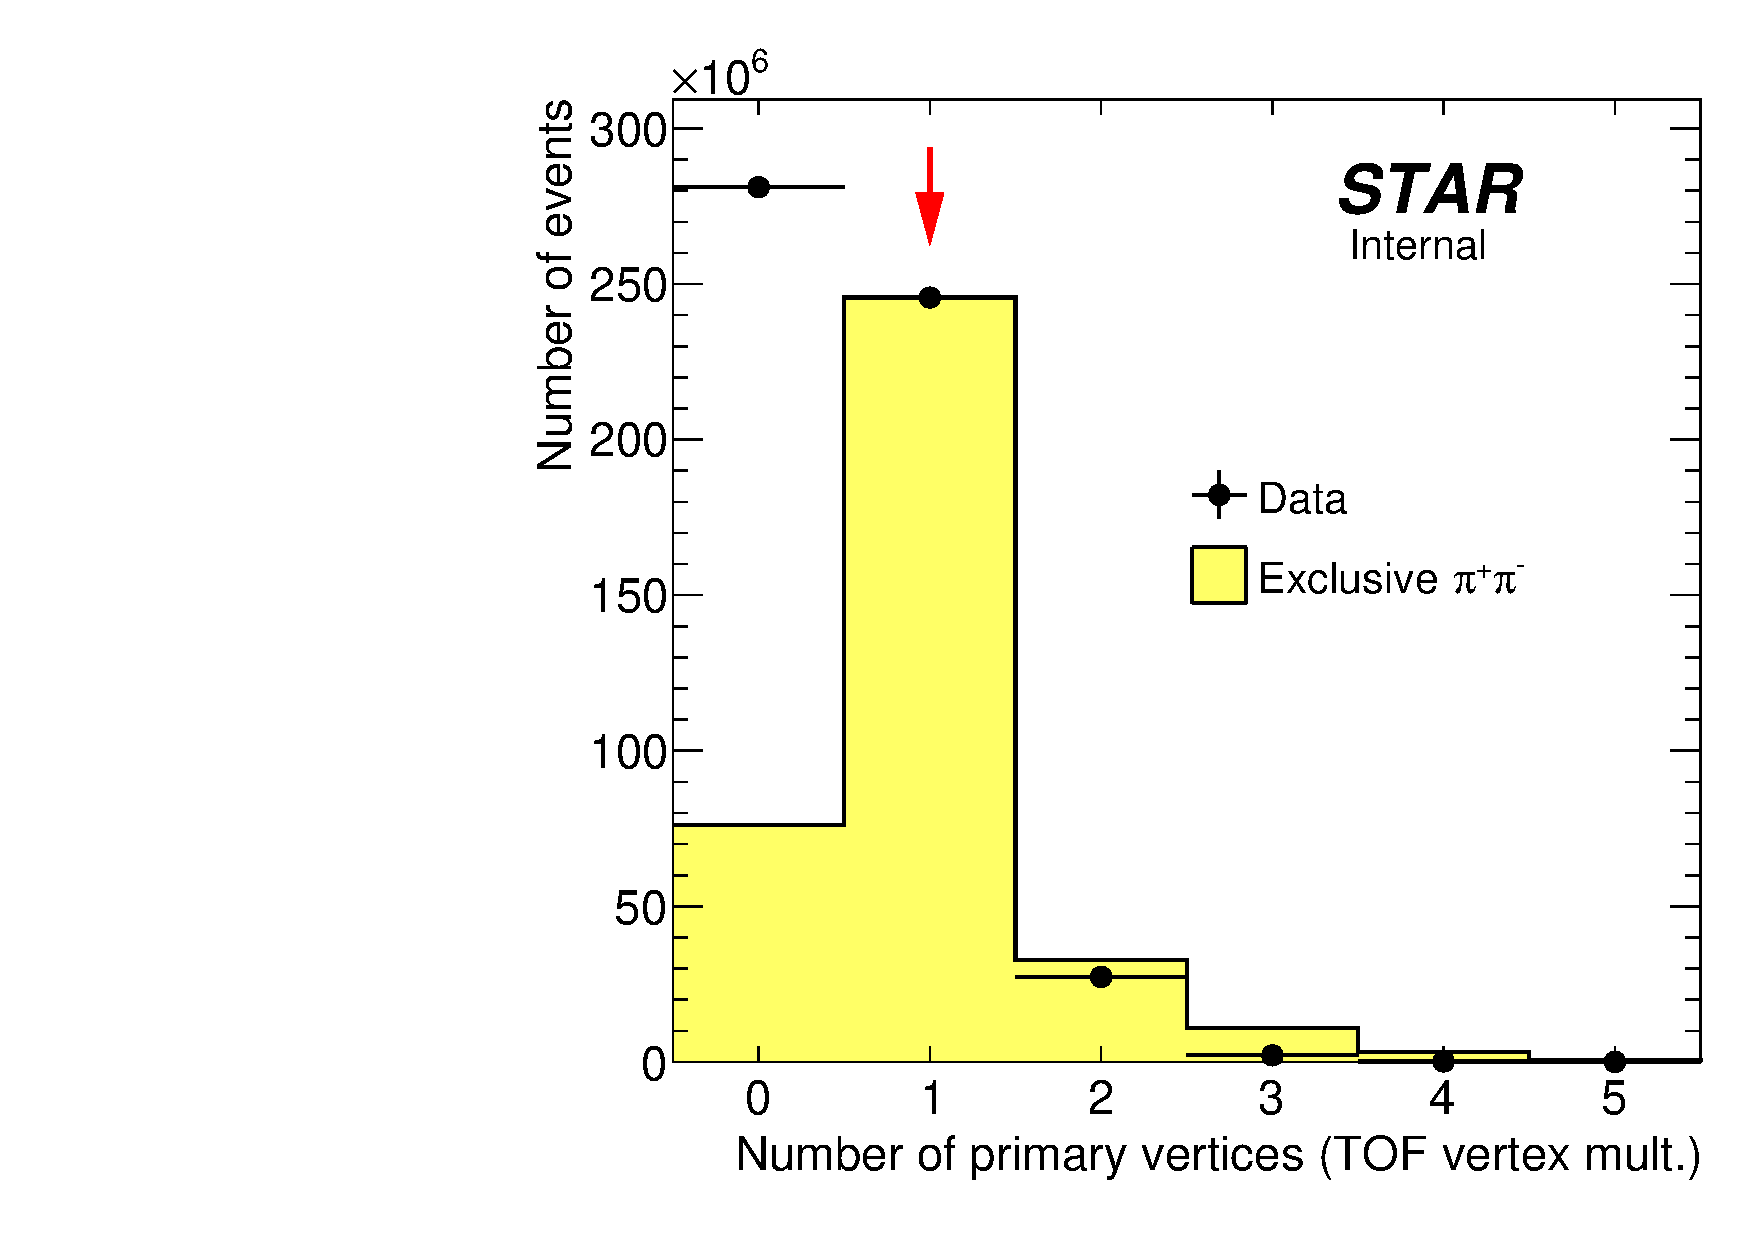
\includegraphics[width=\linewidth]{graphics/eventSelection/NumberOfPrimaryVertices.pdf}%
  \caption{Primary vertex multiplicity. Red arrow marks bin with events with exactly one primary vertex (with track(s) matched with hit in TOF), which are used in physics analysis.}\label{fig:NumberOfPrimaryVertices}
\end{minipage}%
\quad\quad%
\begin{minipage}{.4725\textwidth}%
  \centering
  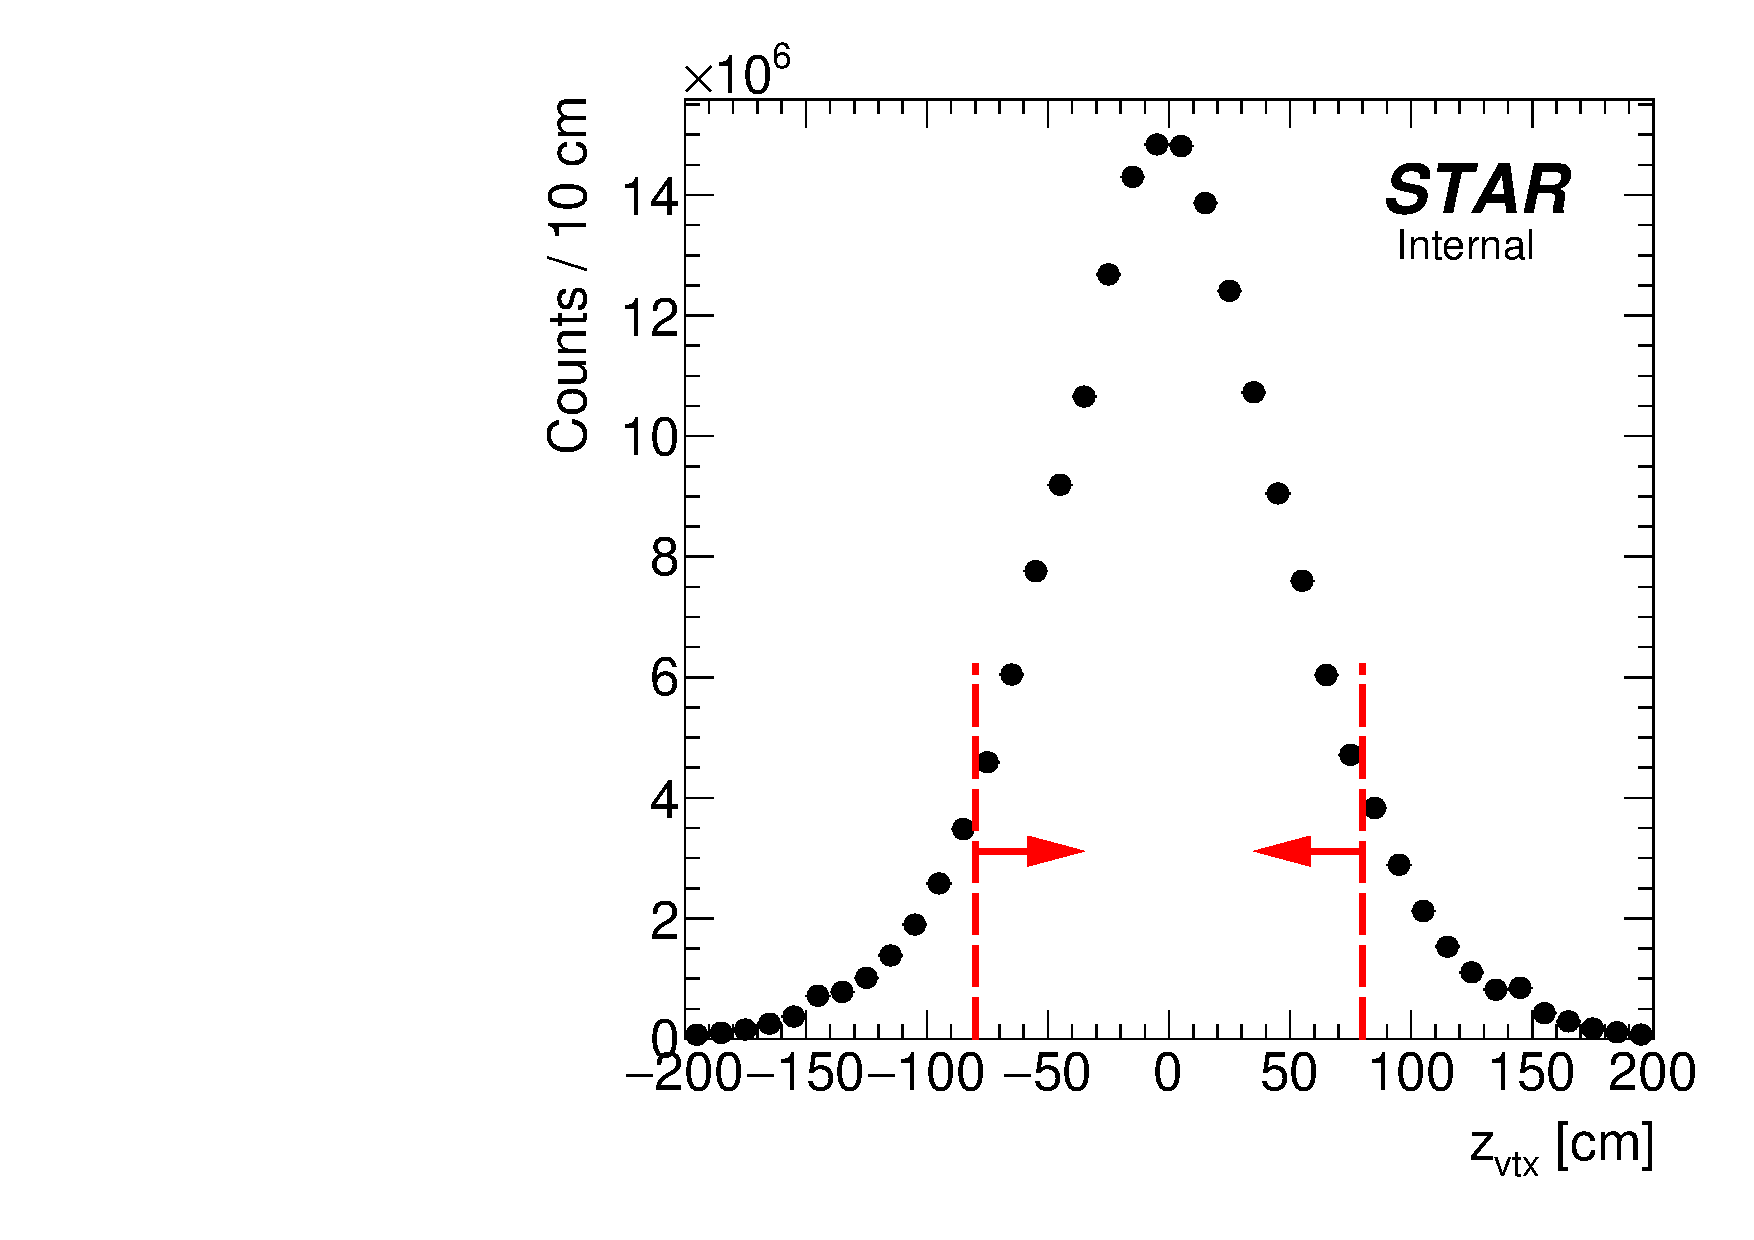
\includegraphics[width=\linewidth]{graphics/eventSelection/zVertex_oneTof.pdf}%
  \caption{\texorpdfstring{$z$}{z}-position of the primary vertex in single TOF vertex events. Red dashed line indicate range of longitudinal vertex position accepted in analysis.\newline}\label{fig:zVertexTpc}
\end{minipage}%
\end{figure}%
%---------------------------


The single TOF vertex is required to be placed within a range $(-80~\text{cm},~80~\text{cm})$ along the $z$-axis~(Fig.~\ref{fig:zVertexTpc}). Events with vertices away from the nominal IP have low acceptance both for the central tracks and the forward protons (comparing to events with vertices close to nominal IP), therefore we reject them as their inclusion to analysis would naturally introduce large systematic uncertainties. See Sec.~3.2.3 in Ref.~\cite{supplementaryNote}



















\subsection{(\ref{enum:CutTpcTrks})~TPC tracks}

The TPC track selection starts from the selection of events with exactly two primary tracks matched with hit in TOF~(Fig.~\ref{fig:NumberOfTofTracksInSingleTofVertex}). Matching with TOF guarantee that analyzed tracks originate from the triggered bunch crossing (ensures that tracks are ''in-time``). It is in accordance with the trigger logic which required at least 2 L0 TOF hits, as well as it enables more accurate particle identification with merged time-of-flight and $dE/dx$ method, comparing to sole usage of $dE/dx$. Primary tracks not matched with hit in TOF, whose average multiplicity in single TOF vertex is $\sim$8, are hardly distinguished between real and fake (off-time) tracks, which is an additional reason for not analyzing events with only one TOF-matched primary TPC track (the other track might be unmatched due to TOF inefficiency).

%---------------------------
\begin{figure}[t!]%
\centering%
\begin{minipage}{.4725\textwidth}%
  \centering%
  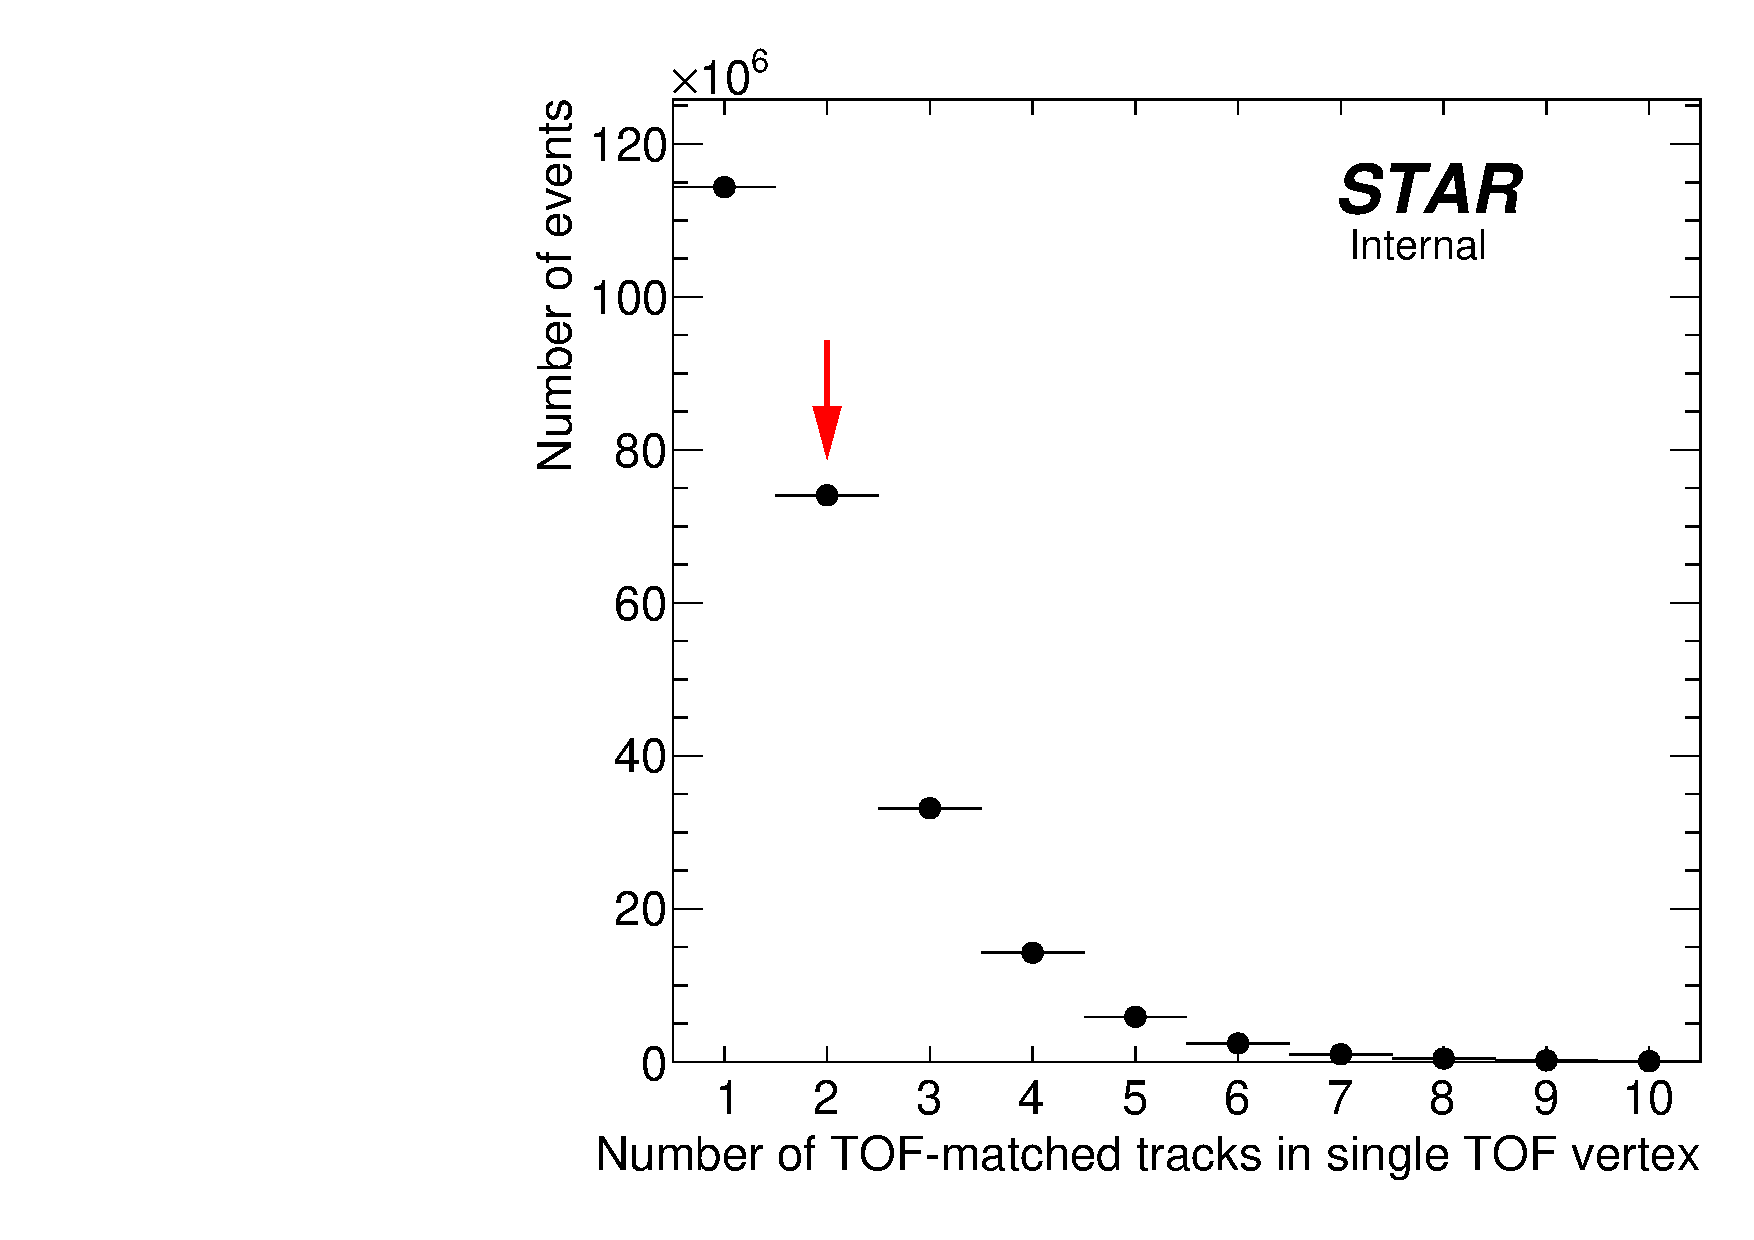
\includegraphics[width=\linewidth]{graphics/eventSelection/TpcTracks/NumberOfTofTracksInSingleTofVertex.pdf}%
  \caption[Multiplicty of primary TPC tracks matched with hit in TOF for single TOF vertex events]{Multiplicty of primary TPC tracks matched with hit in TOF for single TOF vertex events. Red arrow marks bin with events with exactly two primary tracks matched with hit in TOF, which are used in physics analysis.\newline}\label{fig:NumberOfTofTracksInSingleTofVertex}
\end{minipage}%
\quad\quad%
\begin{minipage}{.4725\textwidth}%
  \centering
  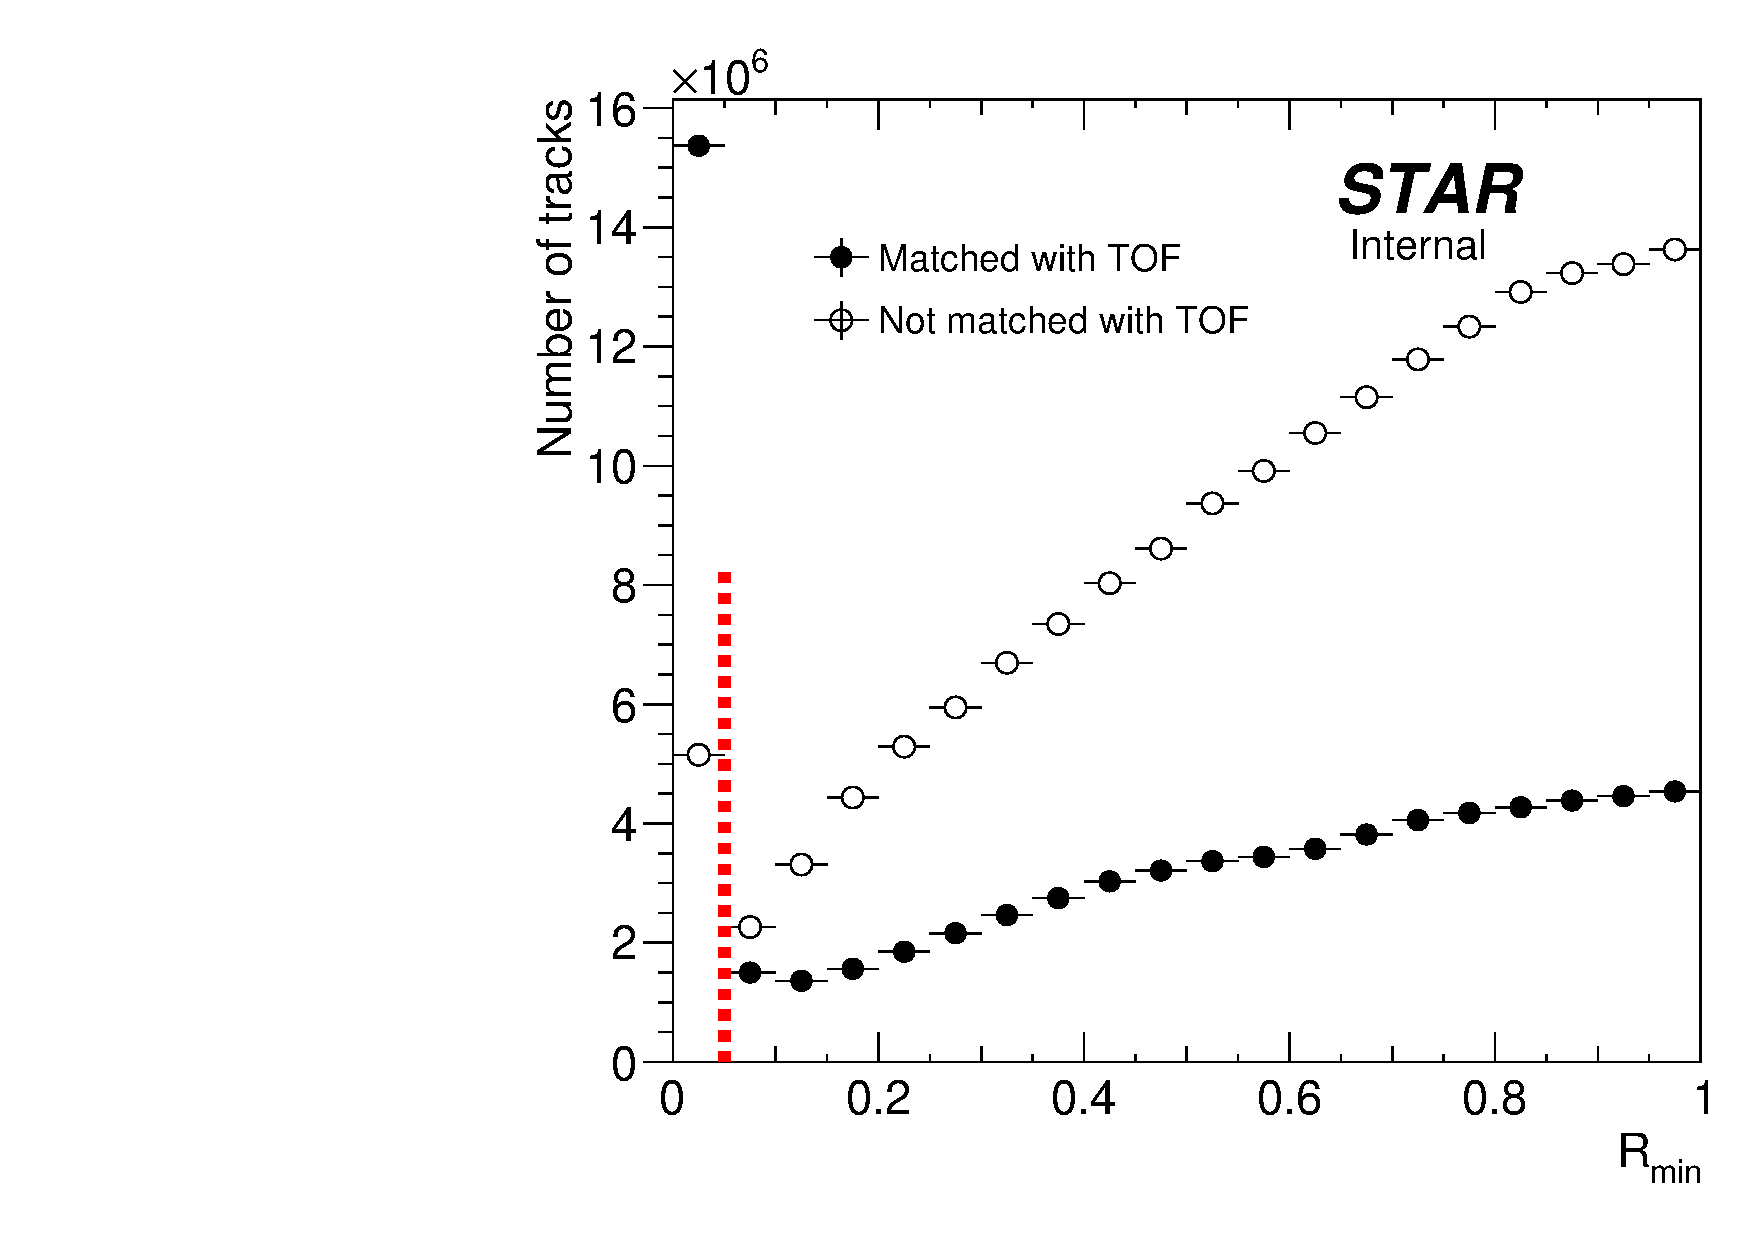
\includegraphics[width=\linewidth]{graphics/eventSelection/TpcTracks/Rmin.pdf}%
  \caption[Distribution of a distance in $\eta-\phi$ space between the BEMC cluster closest to primary TPC track ($R_{\text{min}}$)]{Distribution of a distance in $\eta-\phi$ space between the BEMC cluster closest to primary TPC track matched (filled circle) or not matched (opened circle) with hit in TOF, for single TOF vertex events. Red dashed line indicate matching threshold $R^{\text{match}}_{\text{max}} = 0.05$.}\label{fig:Rmin} %which are expected to reack BEMC
\end{minipage}%
\end{figure}%
%---------------------------

Primary TPC tracks from the single TOF vertex which are matched with TOF are allowed to be also matched with BEMC clusters. Matching with BEMC cluster is claimed if the distance in $\eta-\phi$ space between the BEMC cluster position $(\eta_{\text{clus}},~\phi_{\text{clus}})$ and projected position of the track in BEMC $(\eta_{\text{proj}},~\phi_{\text{proj}})$, defined as
\begin{equation}
 R=\sqrt{(\eta_{\text{clus}}-\eta_{\text{proj}})^{2} + (\phi_{\text{clus}}-\phi_{\text{proj}})^{2}},
\end{equation}
is less than $R^{\text{match}}_{\text{max}} = 0.05$. Distribution of the distance between the primary TPC track and the closest BEMC cluster is shown in~Fig.~\ref{fig:Rmin}.

However, if there are any primary TPC tracks matched with BEMC cluster and not matched with TOF in the single TOF vertex with two TOF-matched tracks, an event is rejected. Such configuration implies higher-than-2 multiplicity of the real tracks in the vertex, hence an event is unlikely a Central Exclusive Production of two particles.



%---------------------------
\begin{figure}[hb]
\centering
\parbox{0.4725\textwidth}{
  \centering
  \begin{subfigure}[b]{\linewidth}
                \subcaptionbox{\label{fig:NHitsFit}}{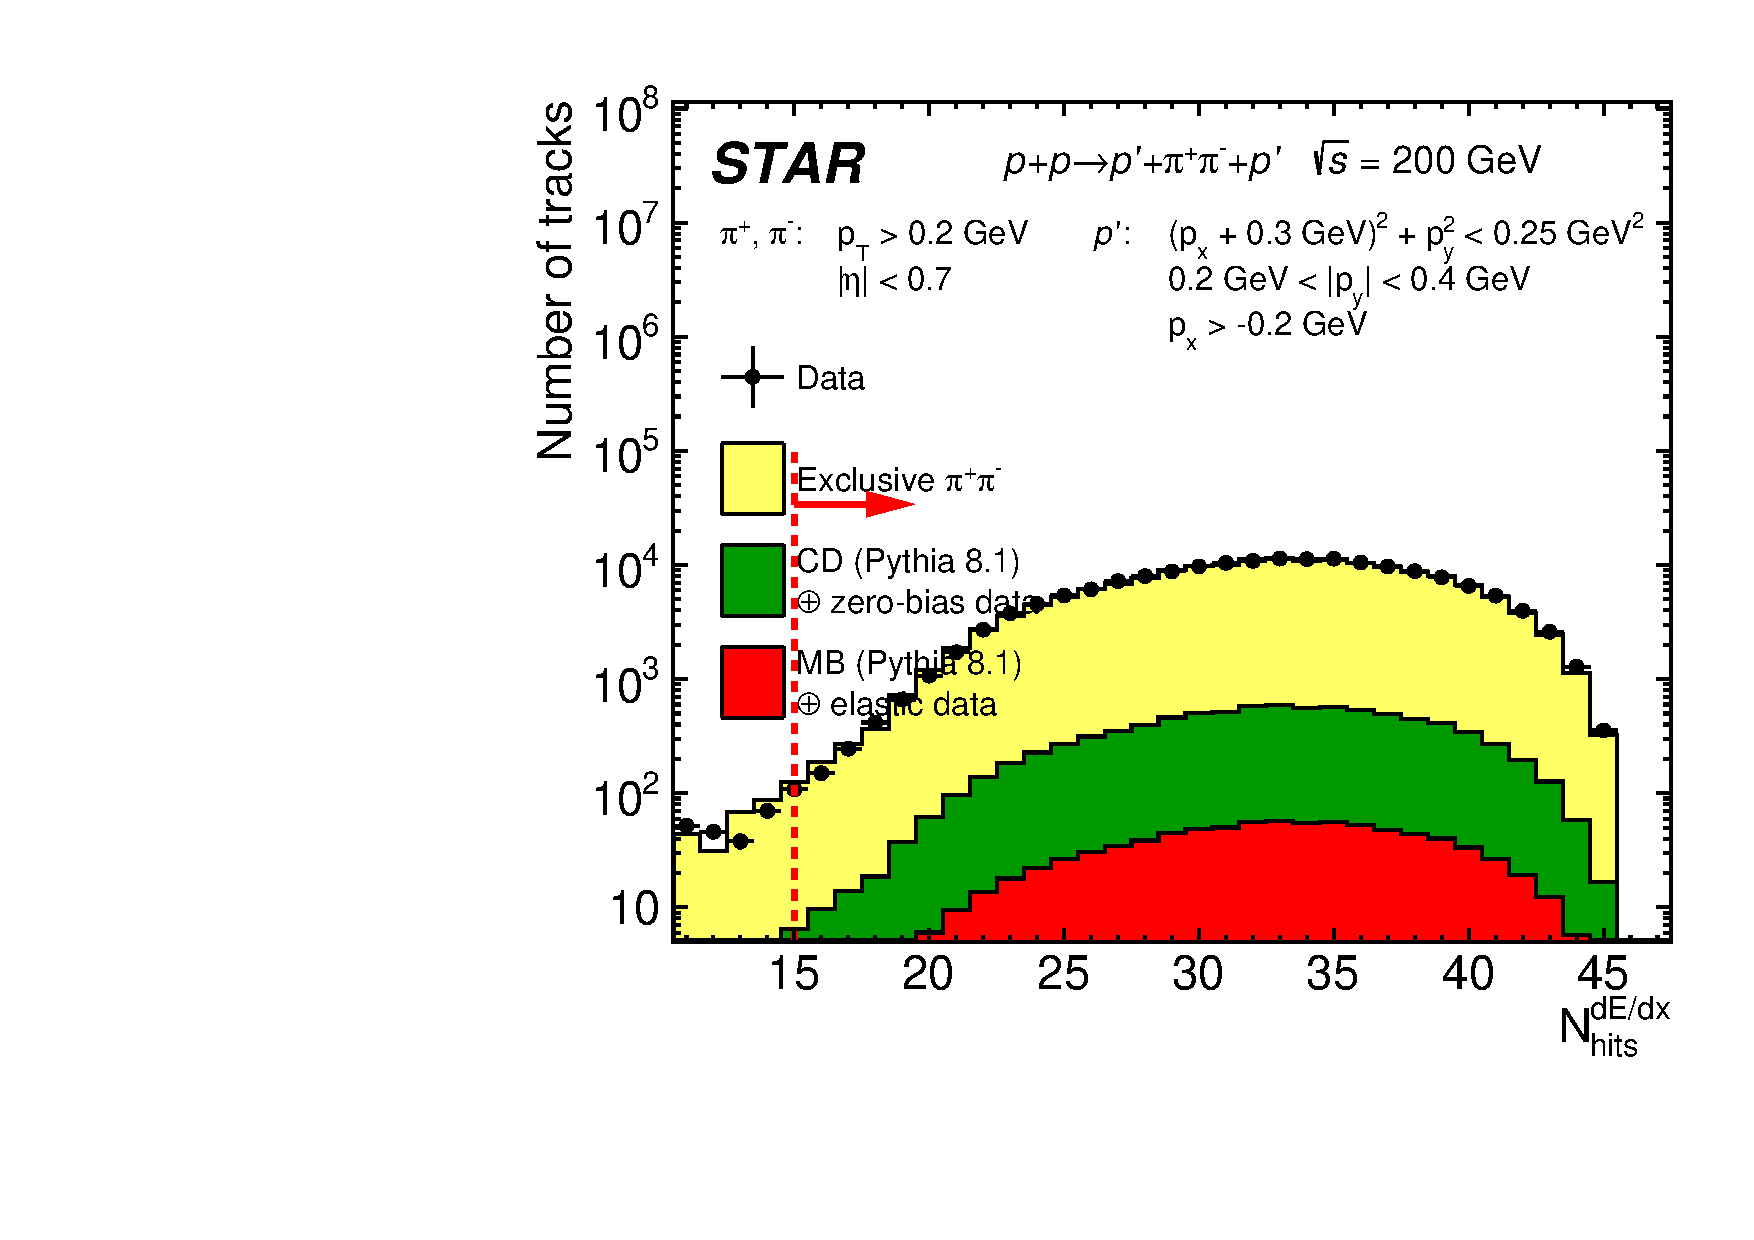
\includegraphics[width=\linewidth]{graphics/eventSelection/TpcTracks/NHitsFit.pdf}}
  \end{subfigure}\\
  \begin{subfigure}[b]{\linewidth}\addtocounter{subfigure}{1}
                \subcaptionbox{\label{fig:NHitsFit_to_NHitsPos}}{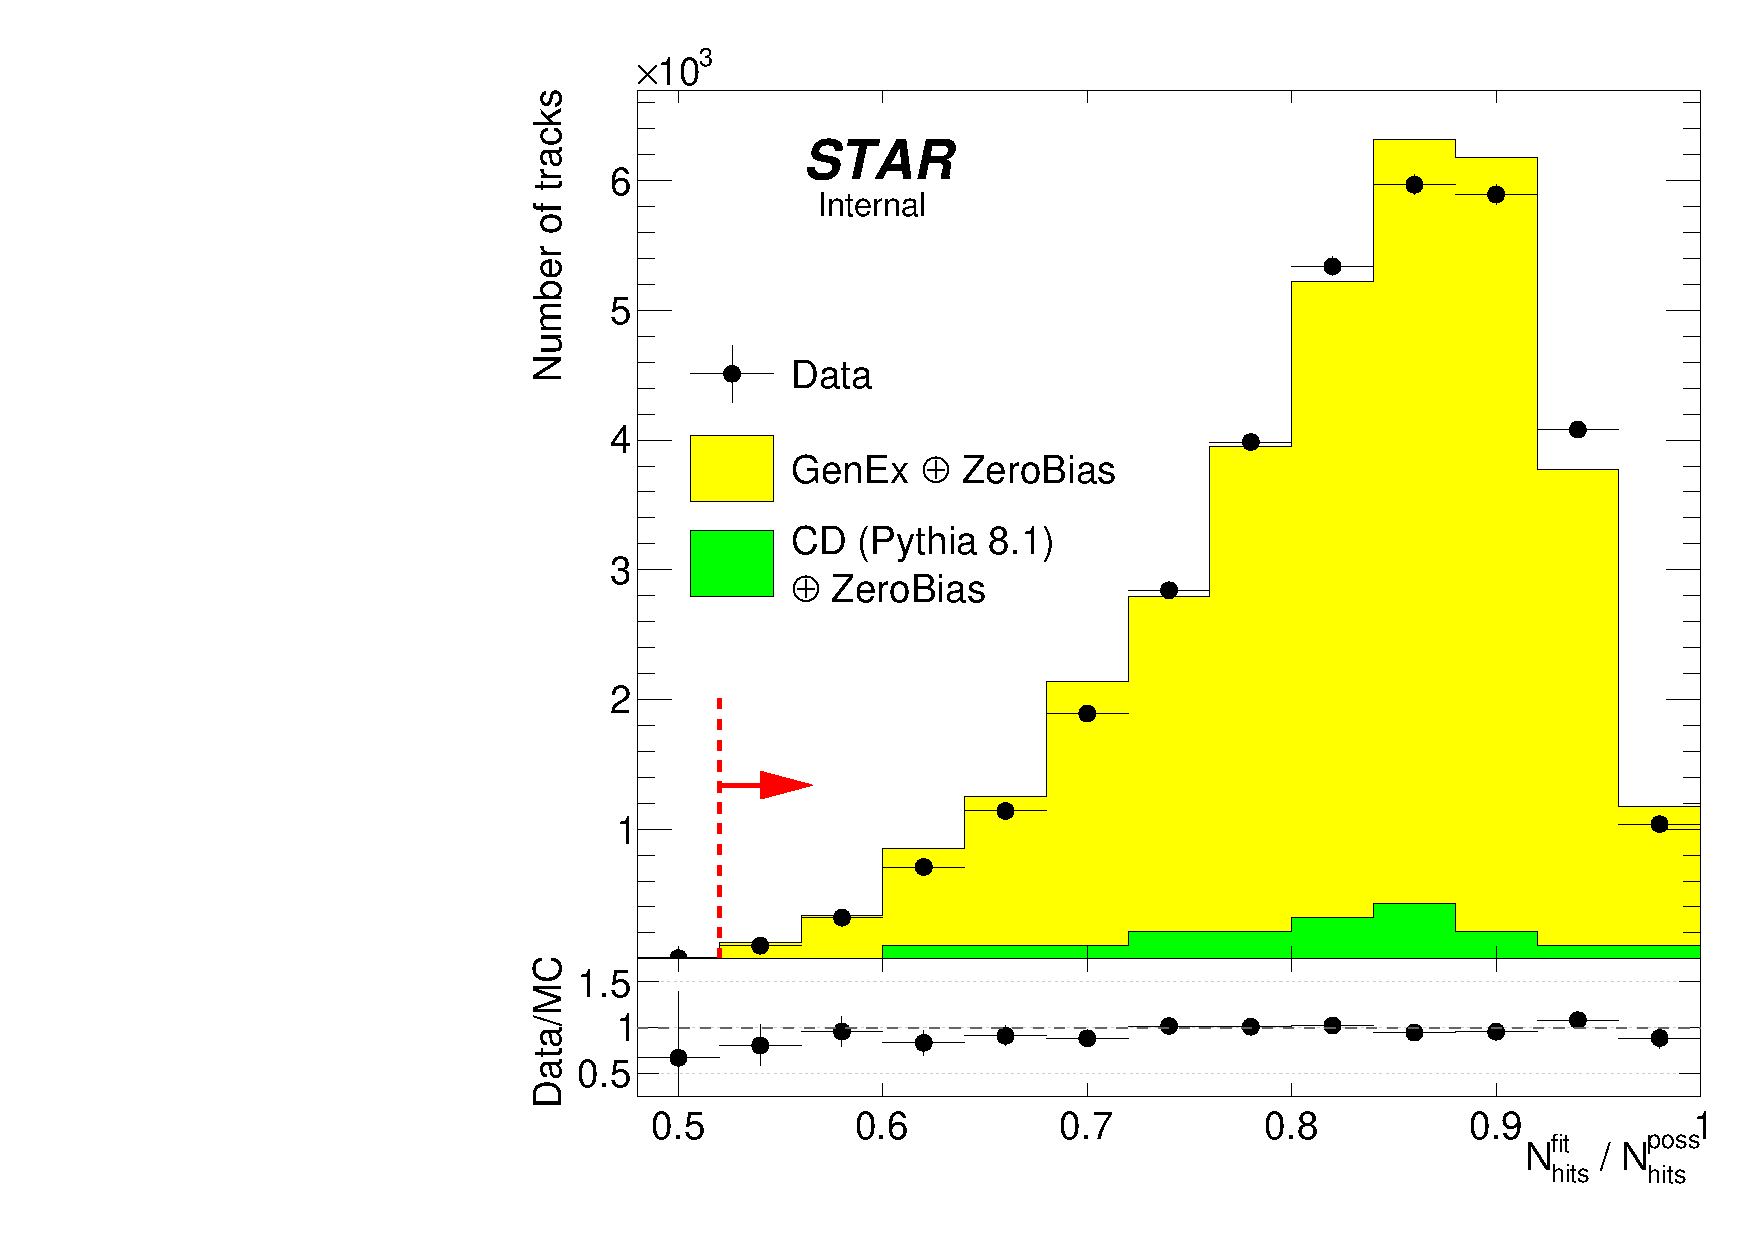
\includegraphics[width=\linewidth]{graphics/eventSelection/TpcTracks/NHitsFit_to_NHitsPos.pdf}}
  \end{subfigure}
}%
\quad\quad%
\parbox{0.4725\textwidth}{
  \centering
  \begin{subfigure}[b]{\linewidth}\addtocounter{subfigure}{-2}
                \subcaptionbox{\label{fig:NHits_dEdx}}{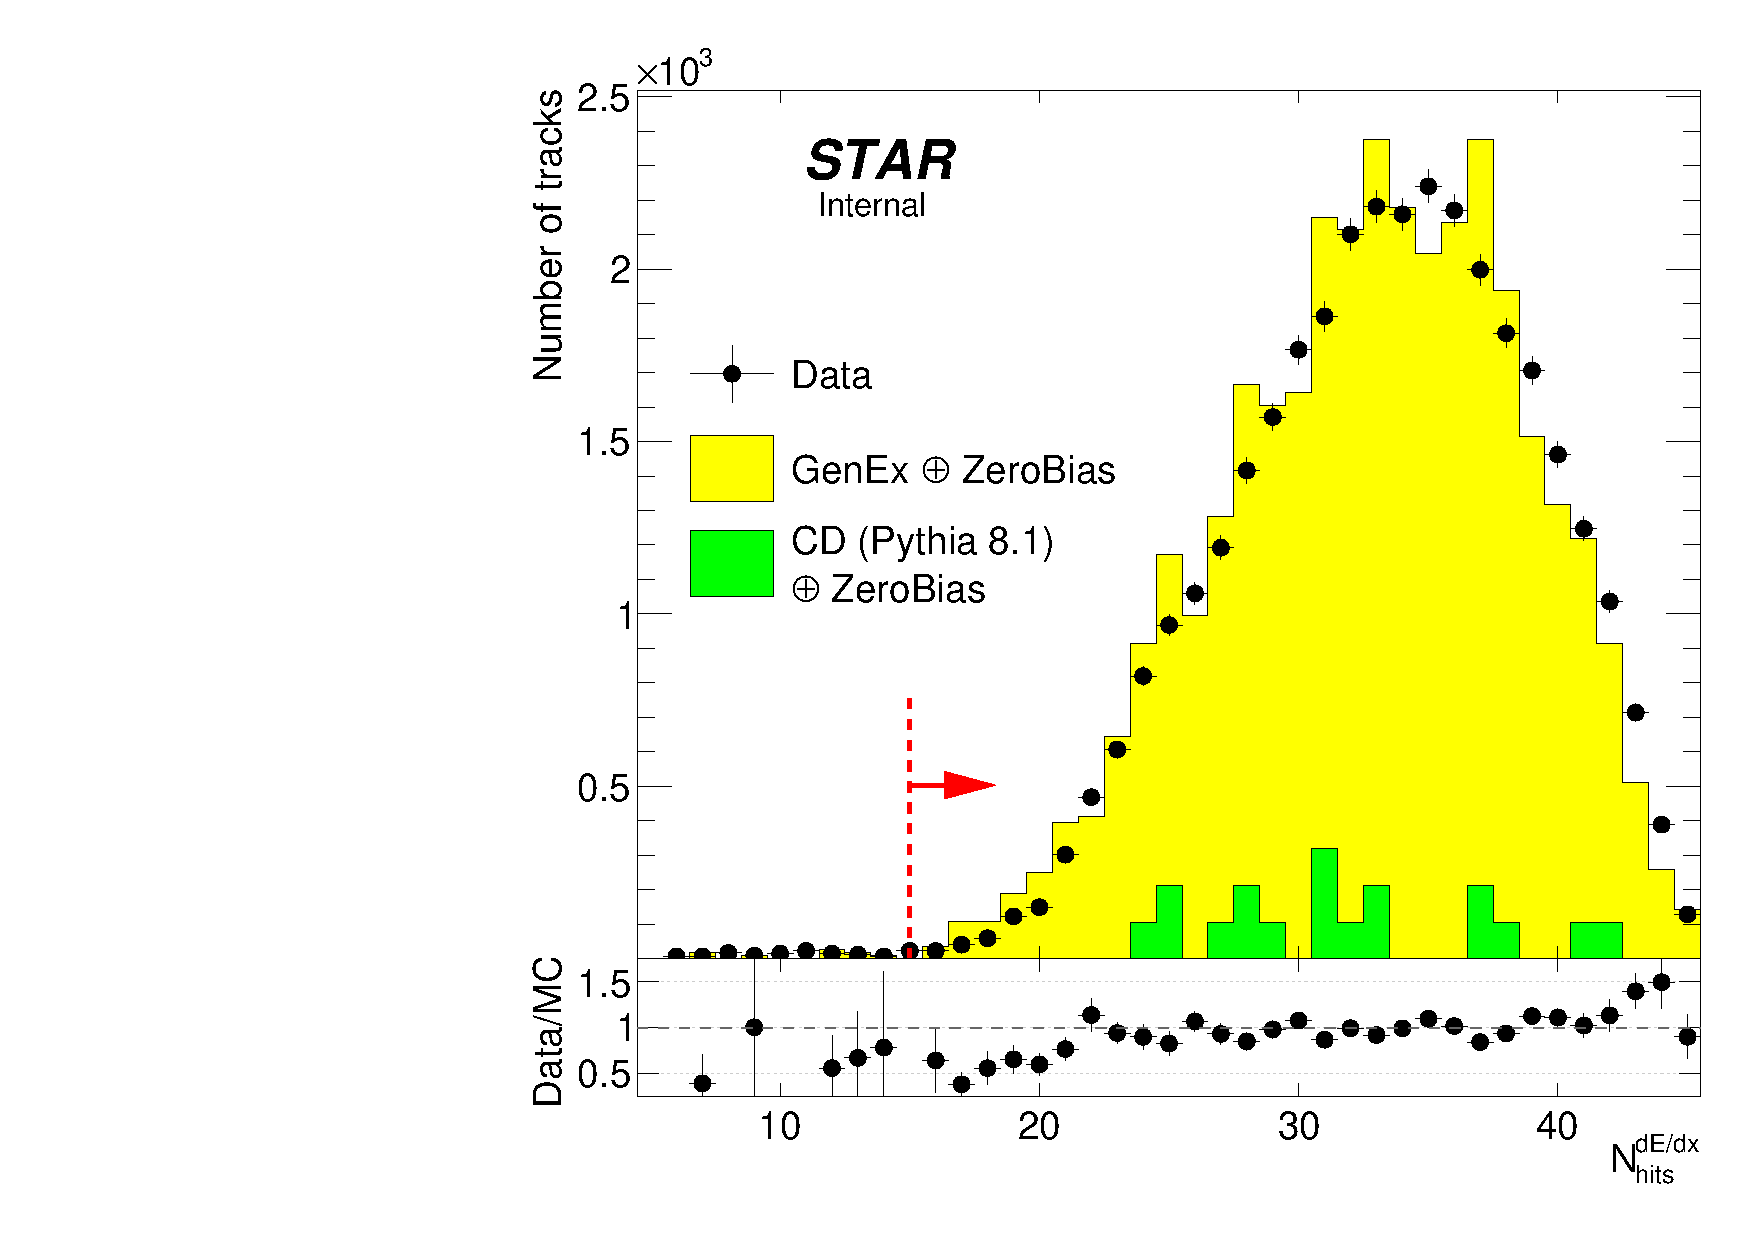
\includegraphics[width=\linewidth]{graphics/eventSelection/TpcTracks/NHits_dEdx.pdf}}
  \end{subfigure}\\
  \begin{minipage}[t][1.042\linewidth][t]{\linewidth}\vspace{10pt}
    \caption[Comparison of distribution of $N_{\text{hits}}^{\text{fit}}$,~$N_{\text{hits}}^{\text{dE/dx}}$ and $N_{\text{hits}}^{\text{fit}}/N_{\text{hits}}^{\text{poss}}$ in the data and embedded MC]
    {Comparison of distribution of the number of hits used in TPC track reconstruction $N_{\text{hits}}^{\text{fit}}$ (\ref{fig:NHitsFit}), number of hits used in specific energy loss reconstruction $N_{\text{hits}}^{\text{dE/dx}}$ (\ref{fig:NHits_dEdx}) and fraction of number of hits potentially generated by the track and finally used in the reconstruction $N_{\text{hits}}^{\text{fit}}/N_{\text{hits}}^{\text{poss}}$ (\ref{fig:NHitsFit_to_NHitsPos}) in the data and embedded MC. Normalizations of the signal and backgrounds were established from the comparison of $p_{T}^{\text{miss}}$ and $\Delta\theta$ distributions after full selection (without cut on the presented quantity and without exclusivity cut), as described in Sec.~\ref{sec:bkgdSignalNorm}. Red dashed line and red arrow indicate the range of each quantity which is accepted in analysis.}\label{fig:NHits}
  \end{minipage}
}%

\end{figure}
%---------------------------







% %---------------------------
% \begin{figure}[ht!]
% \centering
% \parbox{0.4725\textwidth}{
%   \centering
%   \begin{subfigure}[b]{\linewidth}{
%                 \subcaptionbox{\label{fig:d0}}{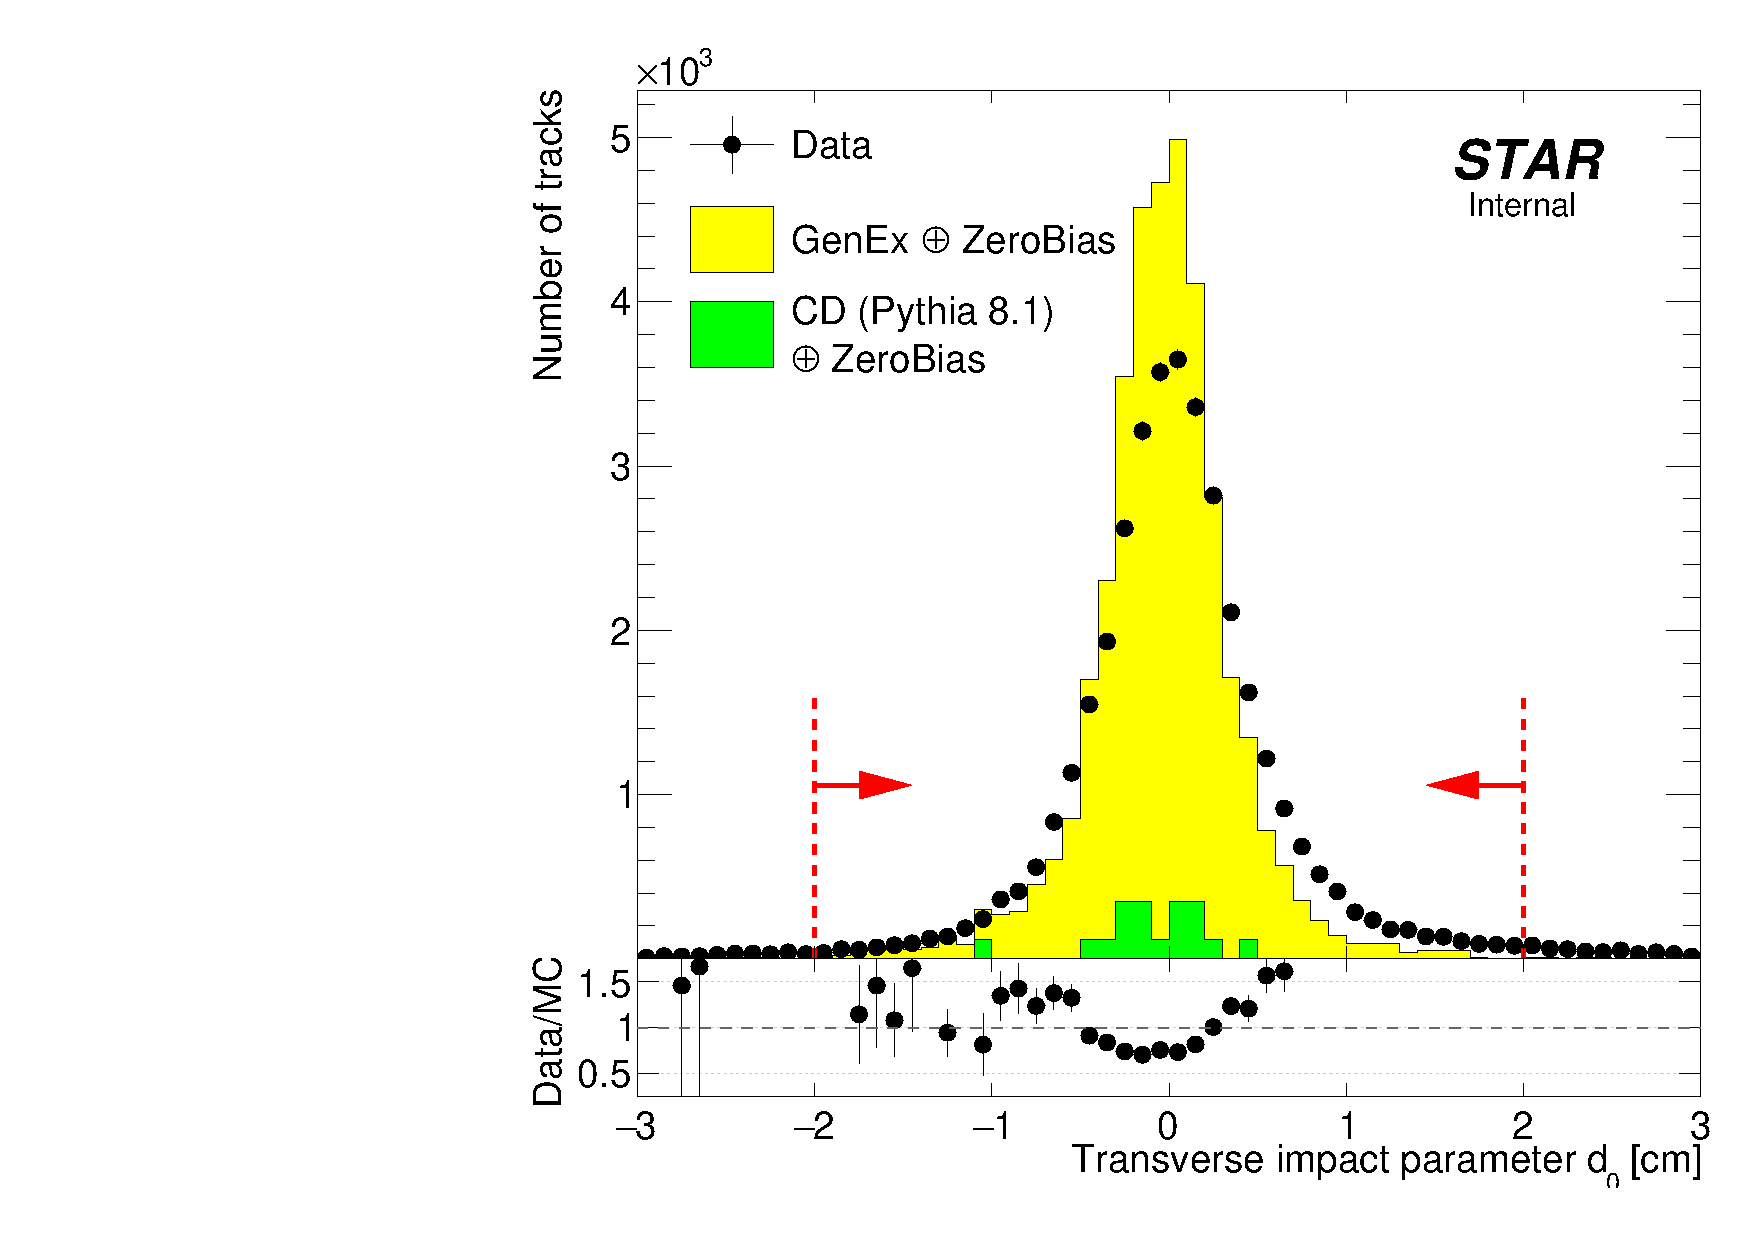
\includegraphics[width=\linewidth]{graphics/eventSelection/TpcTracks/d0.pdf}}}
%   \end{subfigure}
% }%
% \quad\quad%
% \parbox{0.4725\textwidth}{%
%   \centering
%   \begin{subfigure}[b]{\linewidth}{
%                 \subcaptionbox{\label{fig:z0}}{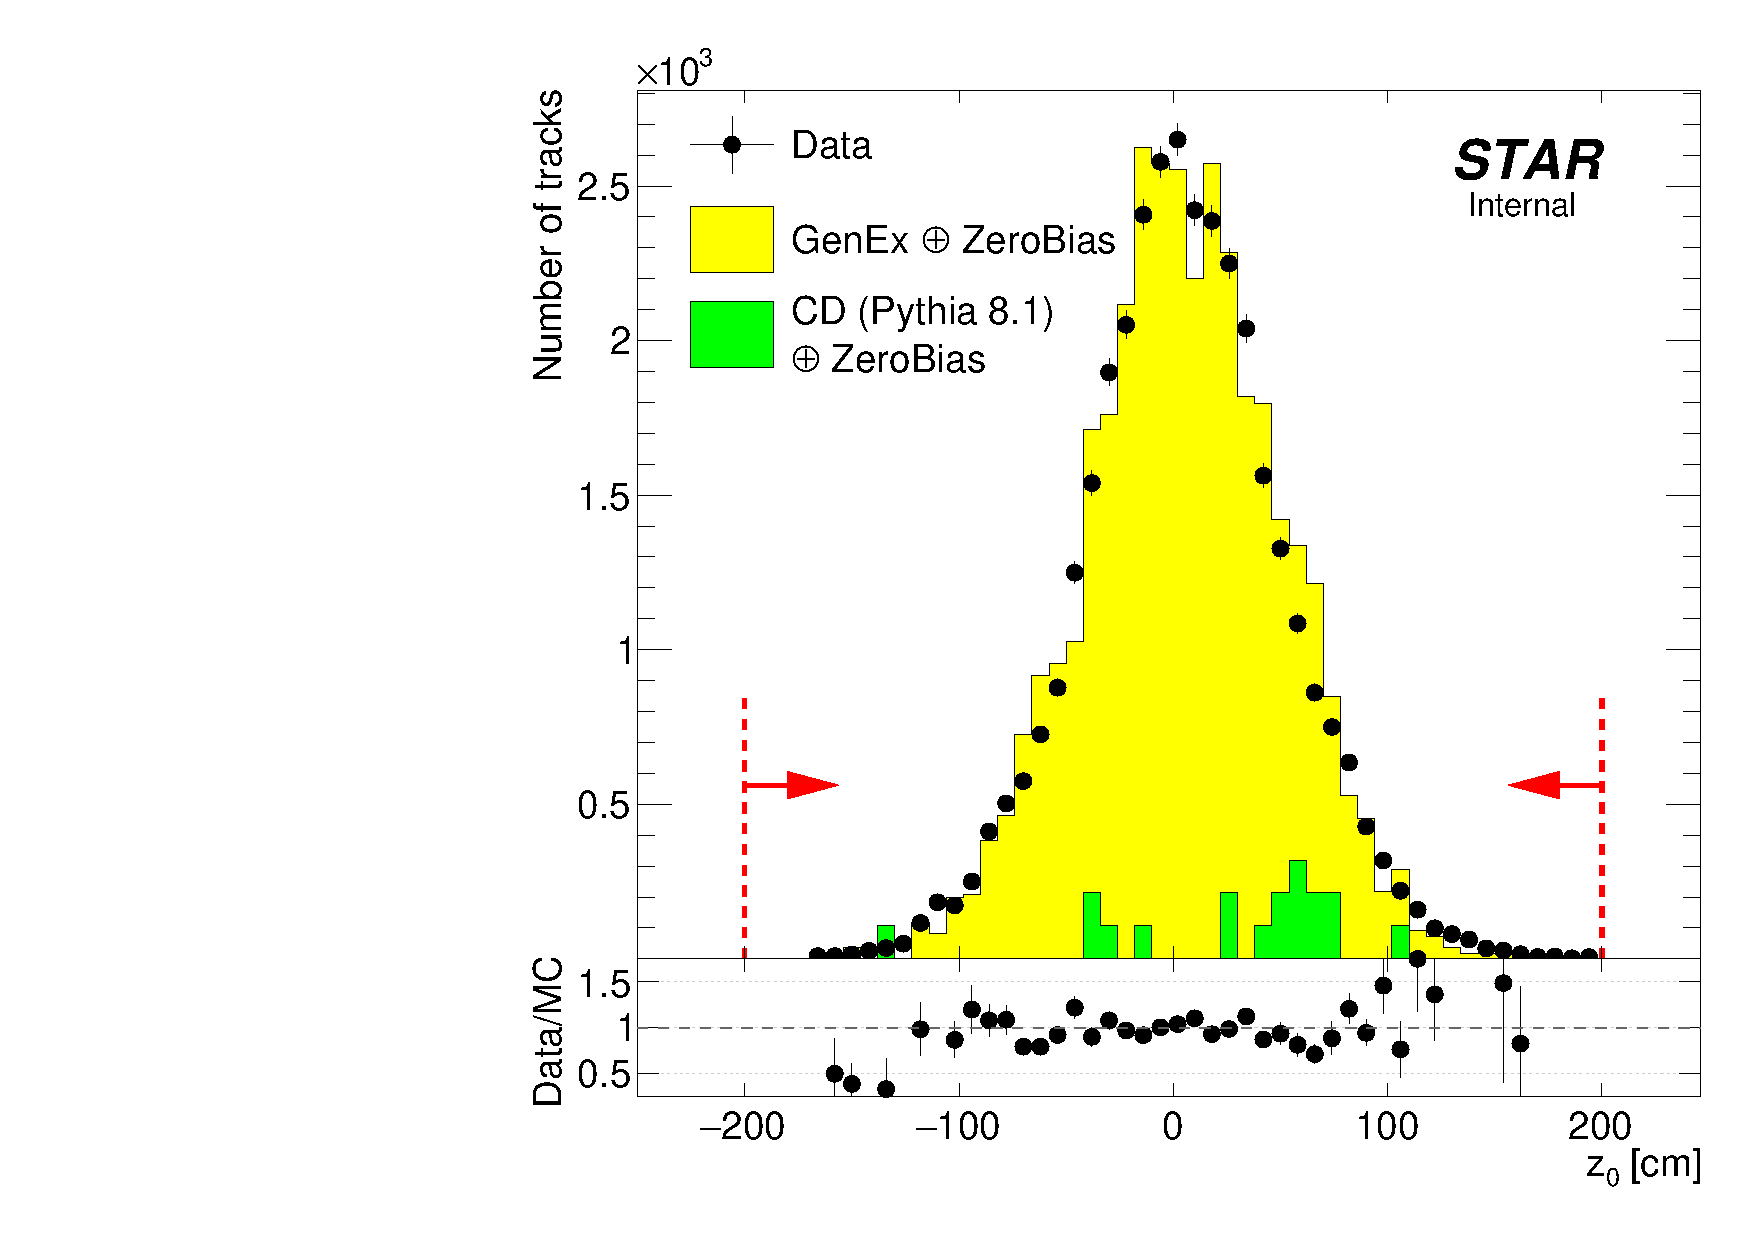
\includegraphics[width=\linewidth]{graphics/eventSelection/TpcTracks/z0.pdf}}}
%   \end{subfigure}
% }%
% \caption[Comparison of distribution of $d_{0}$ and $z_{0}$ in the data and embedded MC]
% {Comparison of distribution of the transverse impact parameter $d_{0}$ (\ref{fig:d0}) and the longitudinal impact parameter $z_{0}$ (\ref{fig:z0}) in the data and embedded MC. Normalizations of the signal and backgrounds were established from the comparison of $p_{T}^{\text{miss}}$ and $\Delta\theta$ distributions after full selection (without cut on the presented quantity and without exclusivity cut), as described in Sec.~\ref{sec:bkgdSignalNorm}. Red dashed lines and red arrows indicate the range of each quantity which is accepted in analysis.}\label{fig:d0z0}
% \end{figure}
% %---------------------------





% 
% %---------------------------
% \begin{figure}[ht!]
% \centering
% \parbox{0.4725\textwidth}{
%   \centering
%   \begin{subfigure}[b]{\linewidth}{
%                 \subcaptionbox{\label{fig:RadialDca}}{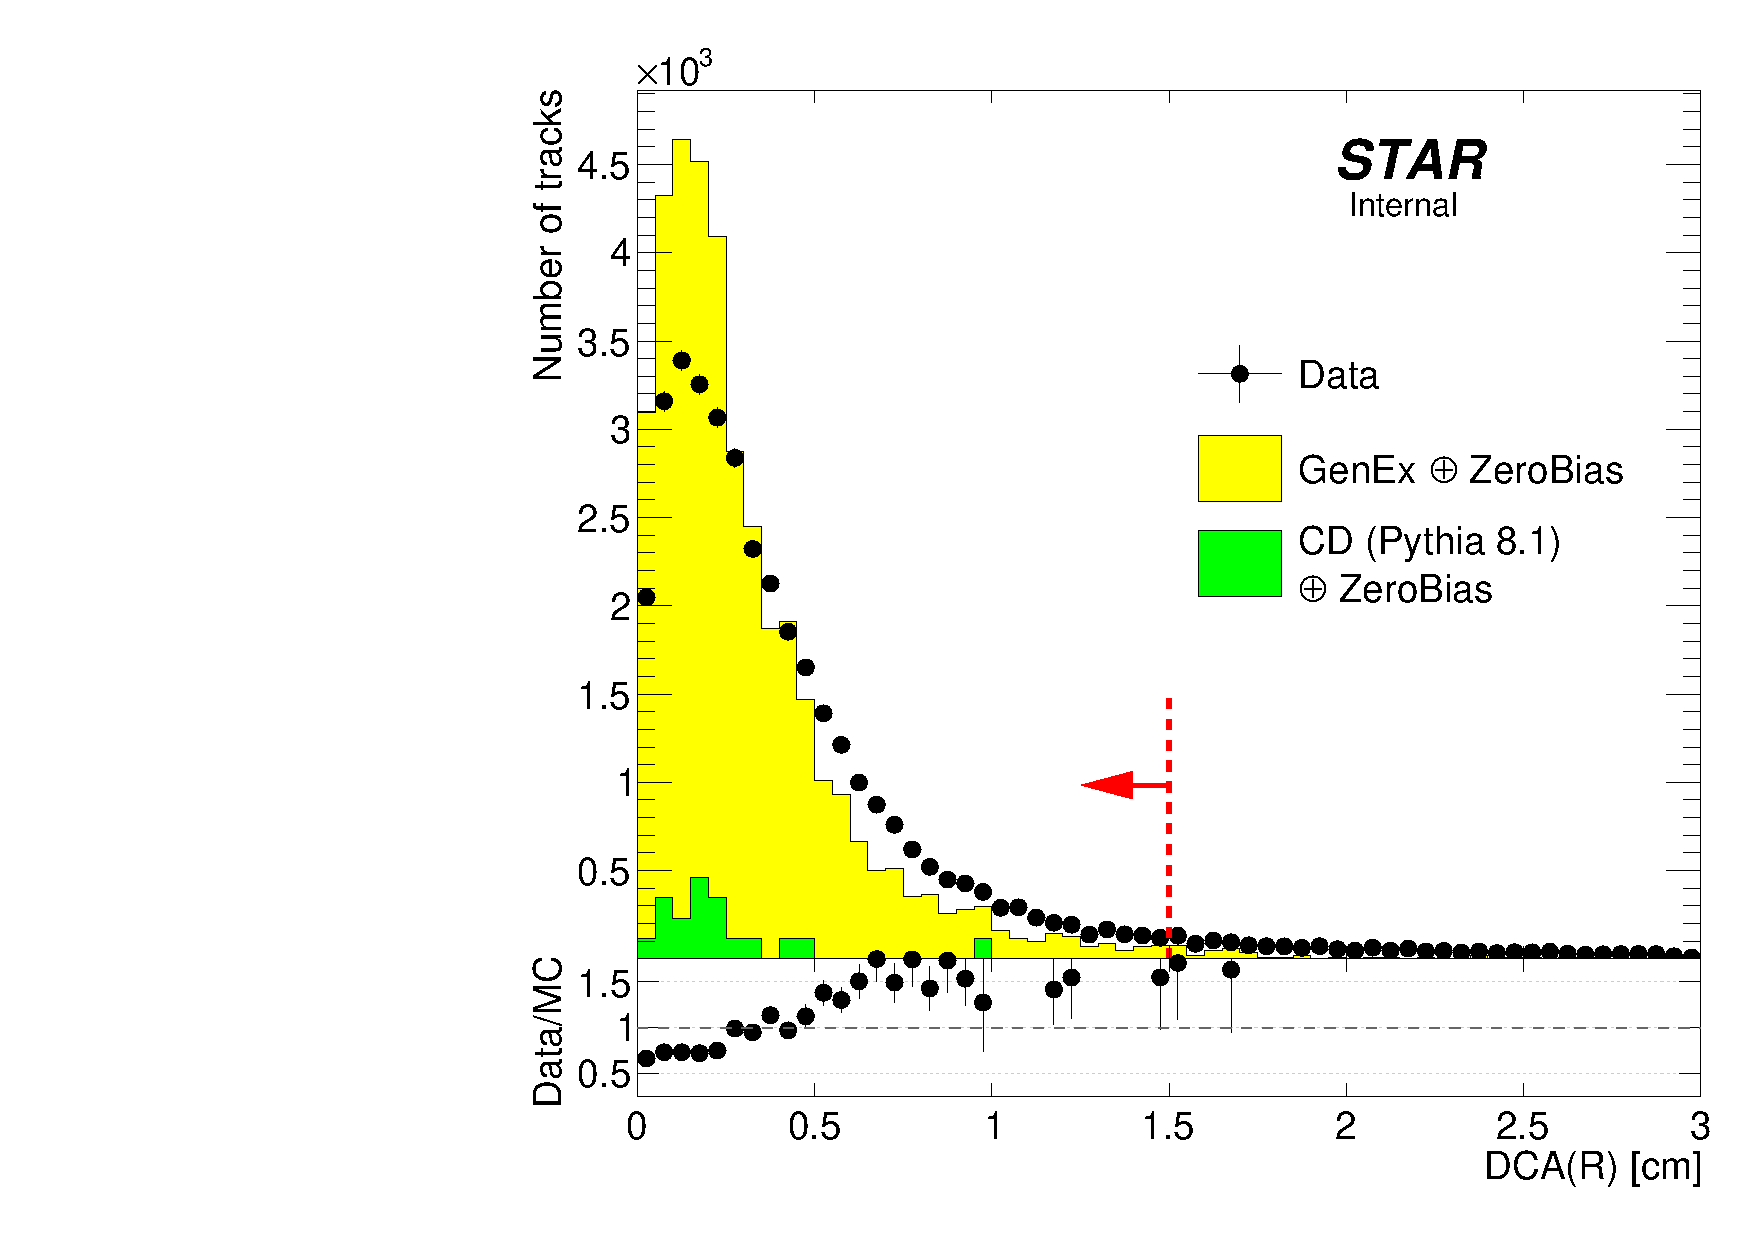
\includegraphics[width=\linewidth]{graphics/eventSelection/TpcTracks/RadialDCA.pdf}}}
%   \end{subfigure}
% }%
% \quad\quad%
% \parbox{0.4725\textwidth}{%
%   \centering
%   \begin{subfigure}[b]{\linewidth}{
%                 \subcaptionbox{\label{fig:LongitudinalDca}}{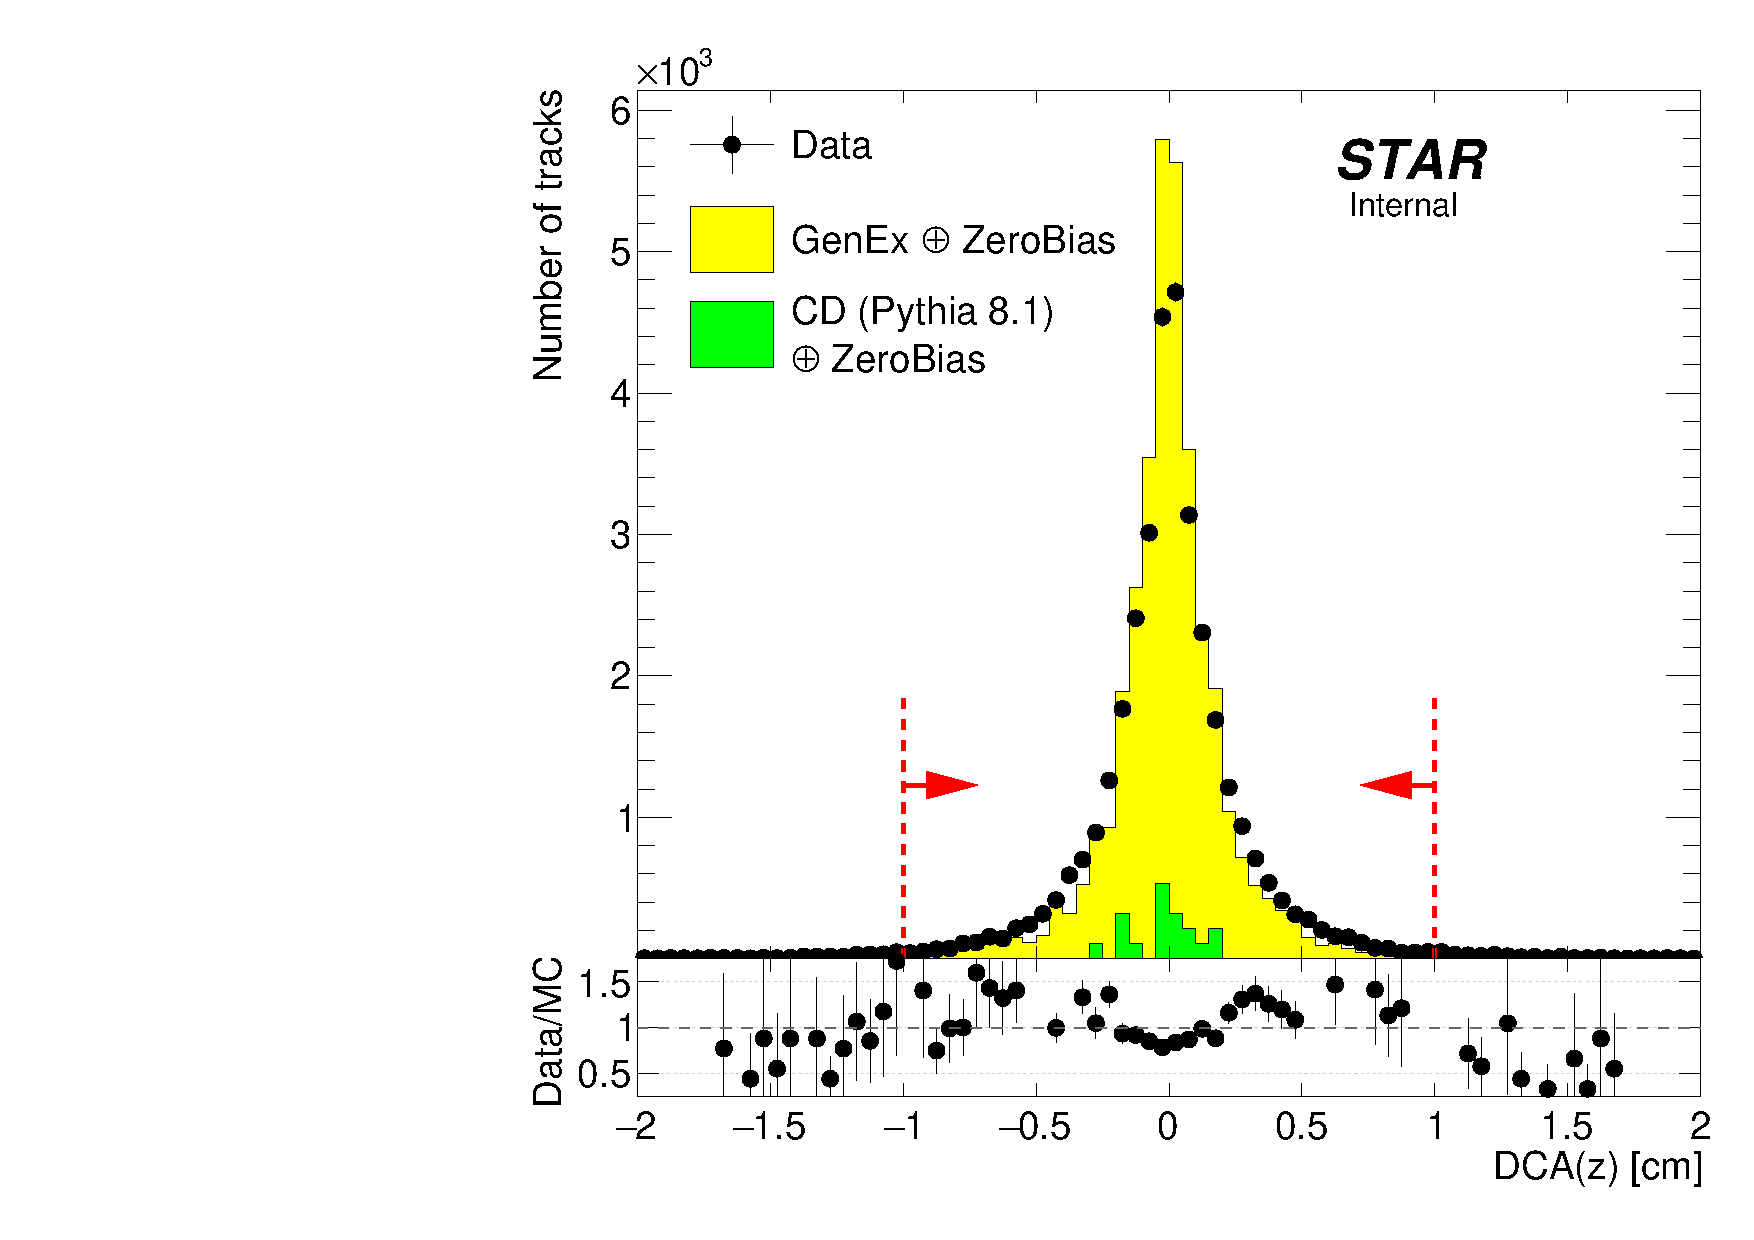
\includegraphics[width=\linewidth]{graphics/eventSelection/TpcTracks/LongitudinalDCA.pdf}}}
%   \end{subfigure}
% }%
% \caption[Comparison of distribution of $\text{DCA}(R)$ and $\text{DCA}(z)$ in the data and embedded MC]
% {Comparison of distribution of the distance of closest approach of the track to the vertex in the $xy$-plane $\text{DCA}(R)$ (\ref{fig:RadialDca}) and the the distance of closest approach of the track to the vertex along the $z$-axis $\text{DCA}(z)$ (\ref{fig:LongitudinalDca}) in the data and embedded MC. Normalizations of the signal and backgrounds were established from the comparison of $p_{T}^{\text{miss}}$ and $\Delta\theta$ distributions after full selection (without cut on the presented quantity and without exclusivity cut), as described in Sec.~\ref{sec:bkgdSignalNorm}. Red dashed lines and red arrows indicate the range of each quantity which is accepted in analysis.}\label{fig:DCA}
% \end{figure}
% %---------------------------



%---------------------------
\begin{figure}[ht!]
\centering
\parbox{0.4725\textwidth}{
  \centering
  \begin{subfigure}[b]{\linewidth}{
                \subcaptionbox{\label{fig:TrackEta}}{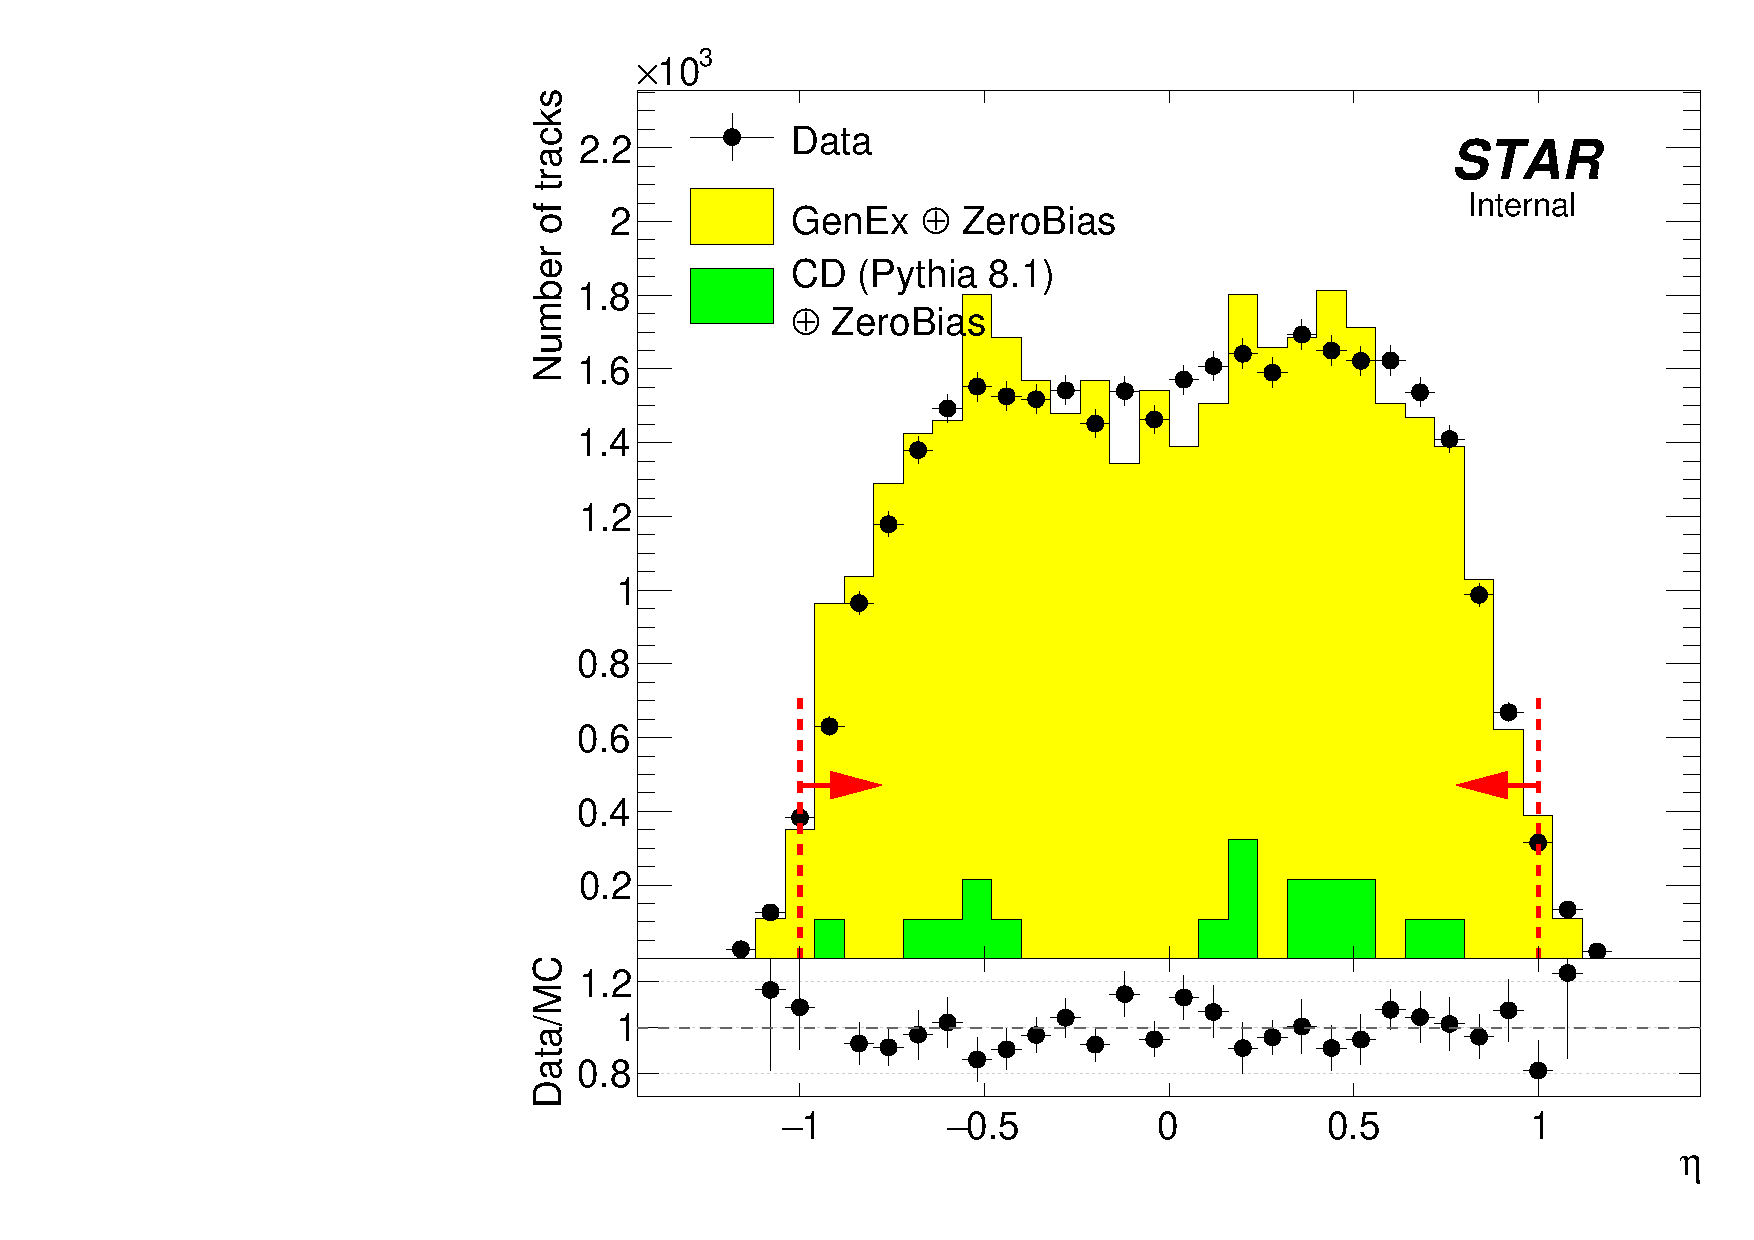
\includegraphics[width=\linewidth]{graphics/eventSelection/TpcTracks/TrackEta.pdf}}}
  \end{subfigure}
}%
\quad\quad%
\parbox{0.4725\textwidth}{%
  \centering
  \begin{subfigure}[b]{\linewidth}{
                \subcaptionbox{\label{fig:TrackPhi}}{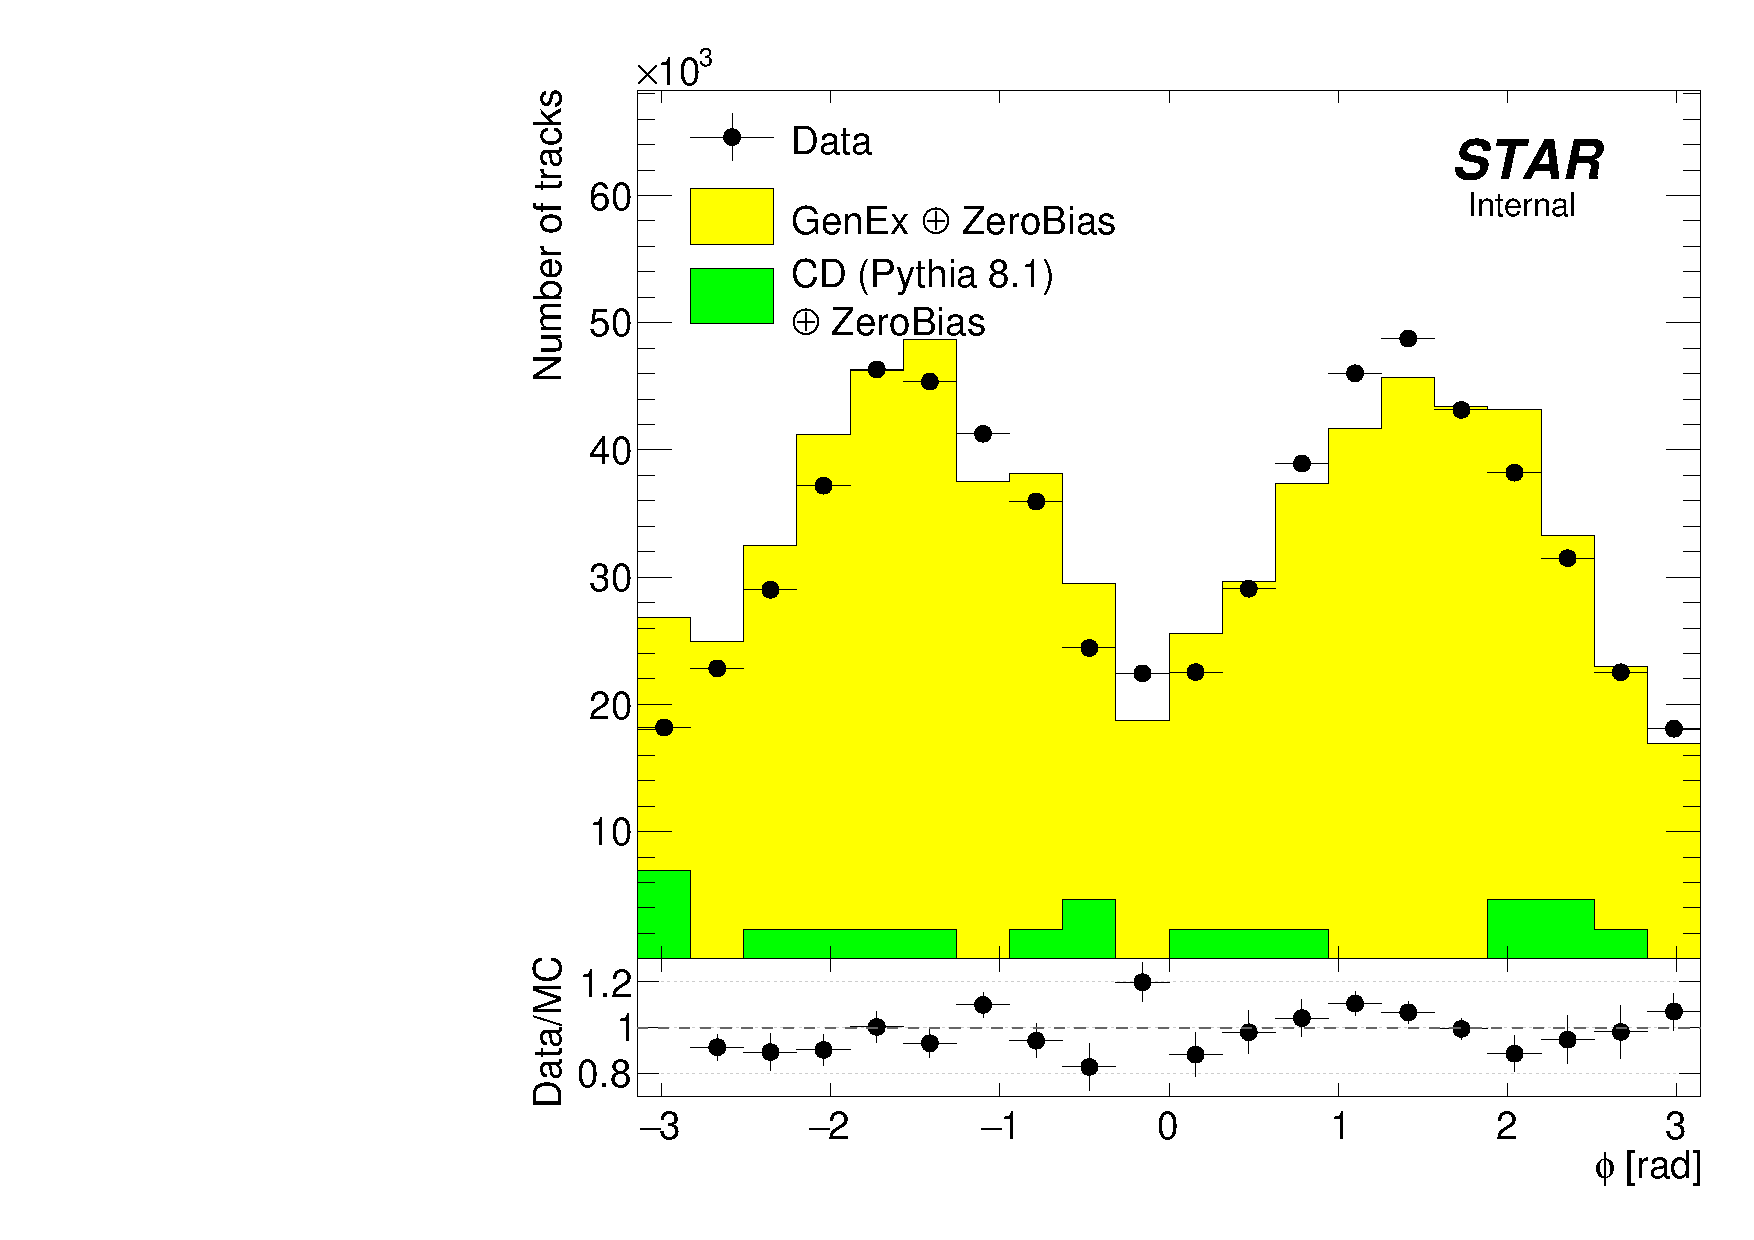
\includegraphics[width=\linewidth]{graphics/eventSelection/TpcTracks/TrackPhi.pdf}}}
  \end{subfigure}
}%
\caption[Comparison of distribution of track $\eta$ and $\phi$ in the data and embedded MC]
{Comparison of the track pseudorapidity $\eta$ (\ref{fig:TrackEta}) and the track azimuthal angle $\phi$ (\ref{fig:TrackPhi}) in the data and embedded MC. Normalizations of the signal and backgrounds were established from the comparison of $p_{T}^{\text{miss}}$ and $\Delta\theta$ distributions after full selection (without cut on the presented quantity and without exclusivity cut), as described in Sec.~\ref{sec:bkgdSignalNorm}. Red dashed lines and red arrows indicate the range of each quantity which is accepted in analysis.}\label{fig:TrackEtaPhi}
\end{figure}
%---------------------------









\subsection{(\ref{enum:CutRpTrks})~RP tracks}

% %---------------------------
% \begin{figure}[ht!]
% \centering
% \parbox{0.315\textwidth}{
%   \centering
%   \begin{subfigure}[b]{\linewidth}{
%                 \subcaptionbox{\label{fig:LocalAngles_2D}}{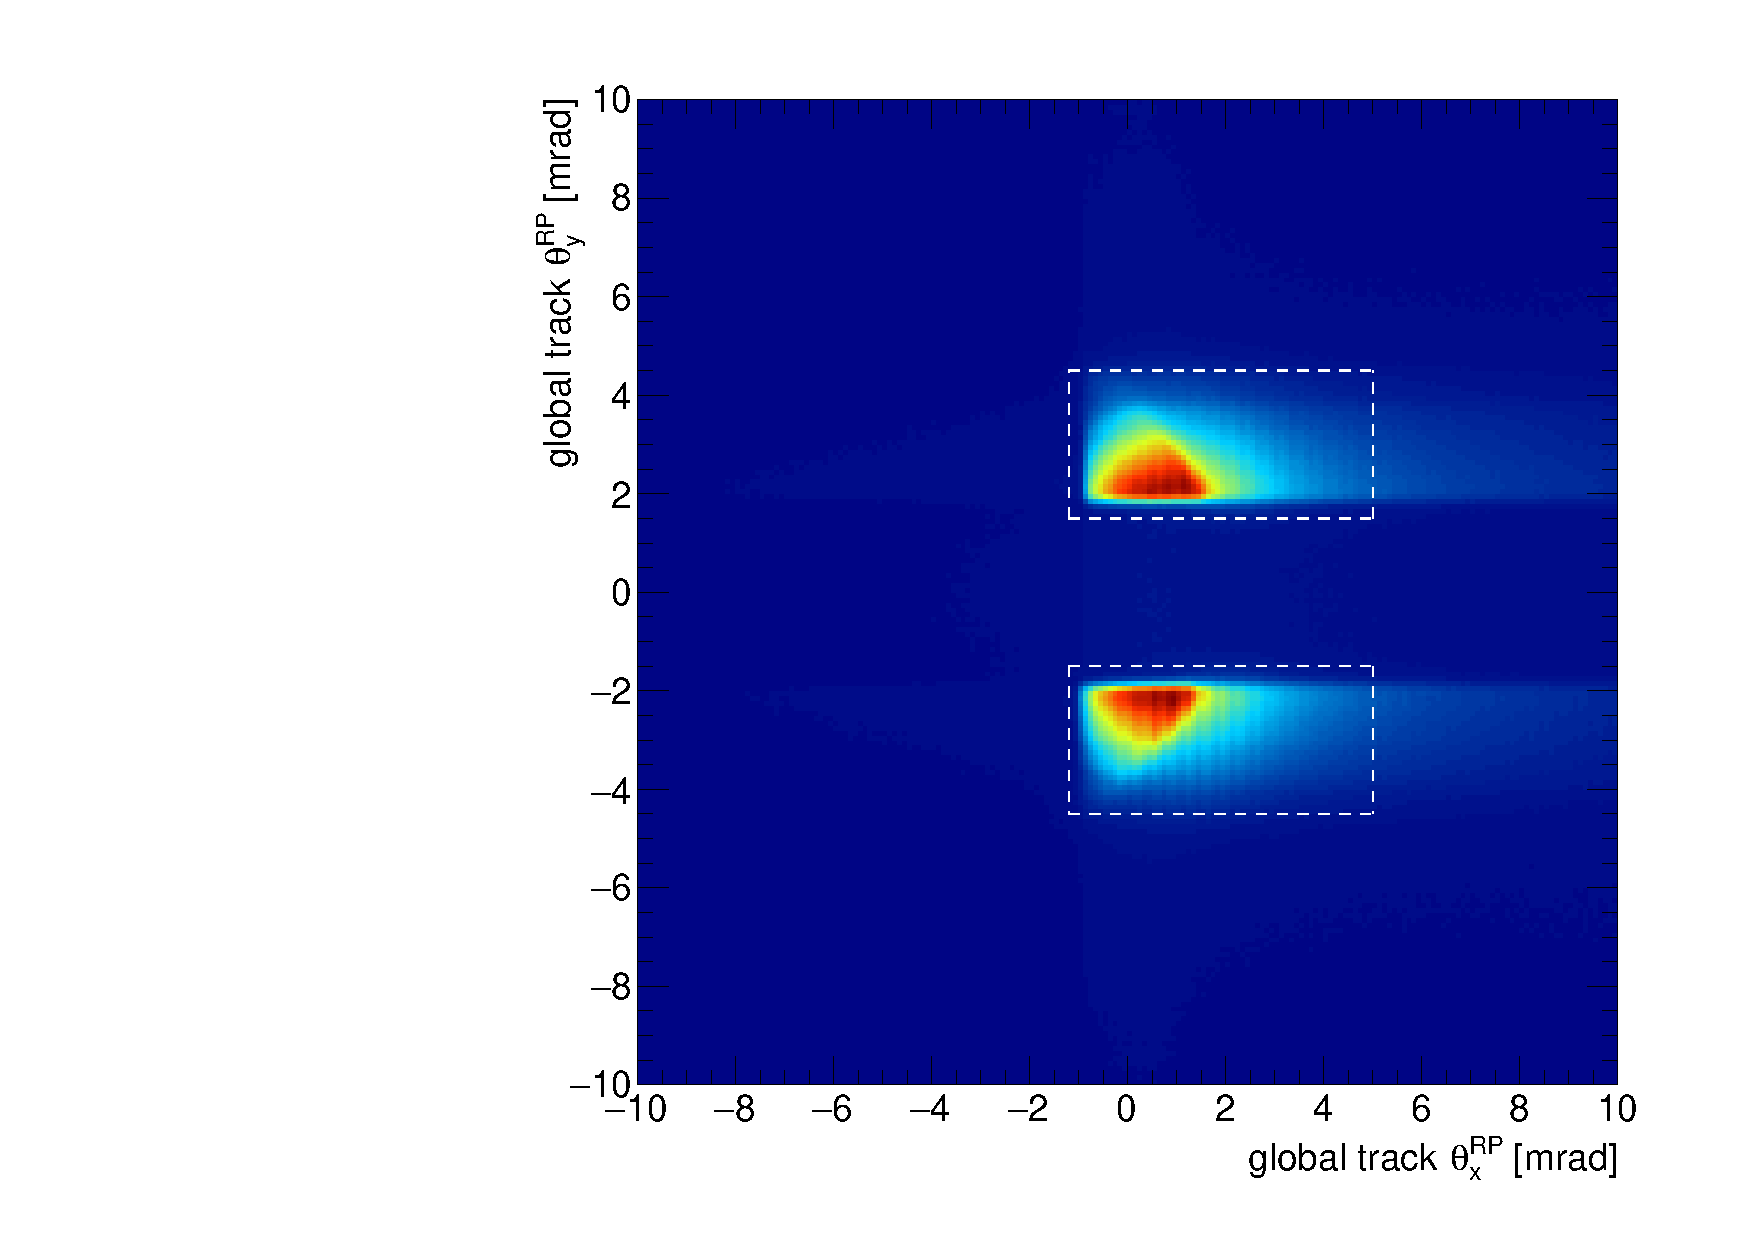
\includegraphics[width=\linewidth,page=1]{graphics/eventSelection/LocalAngles.pdf}}}
%   \end{subfigure}
% }
% \quad
% \parbox{0.315\textwidth}{
%   \centering
%   \begin{subfigure}[b]{\linewidth}{
%                 \subcaptionbox{\label{fig:LocalAngles_1D_x}}{\includegraphics[width=\linewidth,page=2]{graphics/eventSelection/LocalAngles.pdf}}}
%   \end{subfigure}
% }
% \quad
% \parbox{0.315\textwidth}{
%   \centering
%   \begin{subfigure}[b]{\linewidth}{
%                 \subcaptionbox{\label{fig:LocalAngles_1D_y}}{\includegraphics[width=\linewidth,page=3]{graphics/eventSelection/LocalAngles.pdf}}}
%   \end{subfigure}
% }%
% \caption{Local angles of global tracks in Roman Pots.}
% \end{figure}
% %---------------------------
%%%%%%%%%%%%%%%%%%%%%%%%%%%%%%%%%%%%%%%%%%%%%%%%%%%%%%%%%%%%%%%%%%%%%%%%%%%%%%%%%%%%%%%%%%%%%%%%%%%%%%%%%%%%%%%%%%%%%%%%%%%%%%%%%%%%




%%%%%%%%%%%%%%%%%%%%%%%%%%%%%%%%%%%%%%%%%%%%%%%%%%%%%%%%%%%%%%%%%%%%%%%%%%%%%%%%%%%%%%%%%%%%%%%%%%%%%%%%%%%%%%%%%%%%%%%%%%%%%%%%%%%%
\subsection{(\ref{enum:CutDeltaZVx})~TPC-RP \texorpdfstring{$z$}{z}-vertex matching}

In CEP tracks in the central detector and tracks in Roman Pots originate from the same interaction vertex. Measurement of the time of detection of forward protons in RPs gives access to reconstruction of the position of the vertex
\begin{equation}
z_{\text{vtx}}^{\text{RP}} = c\cdot\frac{t^{\text{RP}}_{\text{W}} - t^{\text{RP}}_{\text{E}}}{2}
\end{equation}
independently from TPC, which allows their comparison and rejection of the background if the two values disagree. Time of detection of proton in RP is provided in StMuRpsTrack object - it is an average of all TAC values from PMTs in RPs used to form a track, corrected for the slewing effect and adjusted to have the best correlation with the $z$-position of the vertex measured in TPC, translated to unit of time (all these steps are done at the level of raw data reconstruction). In Fig.~\ref{fig:zVertexRpTpc} the comparisons of the $z_{\text{vtx}}^{\text{RP}}$ and $z_{\text{vtx}}^{\text{TPC}}$ are shown with some preselection cuts applied. A clear signal from the Central Diffraction (and thus CEP) process is manifesting in high correlation of the two values (diagonal in Fig.~\ref{fig:zVertexRpVsTpc}) or significant and relatively narrow peak centered at 0 for the difference of two values (Fig.~\ref{fig:zVertexRpMinusZVertexTpc}). %
%---------------------------
\begin{figure}[ht!]
\centering
\parbox{0.4\textwidth}{
  \centering
  \begin{subfigure}[b]{\linewidth}{
                \subcaptionbox{\label{fig:zVertexRpVsTpc}}{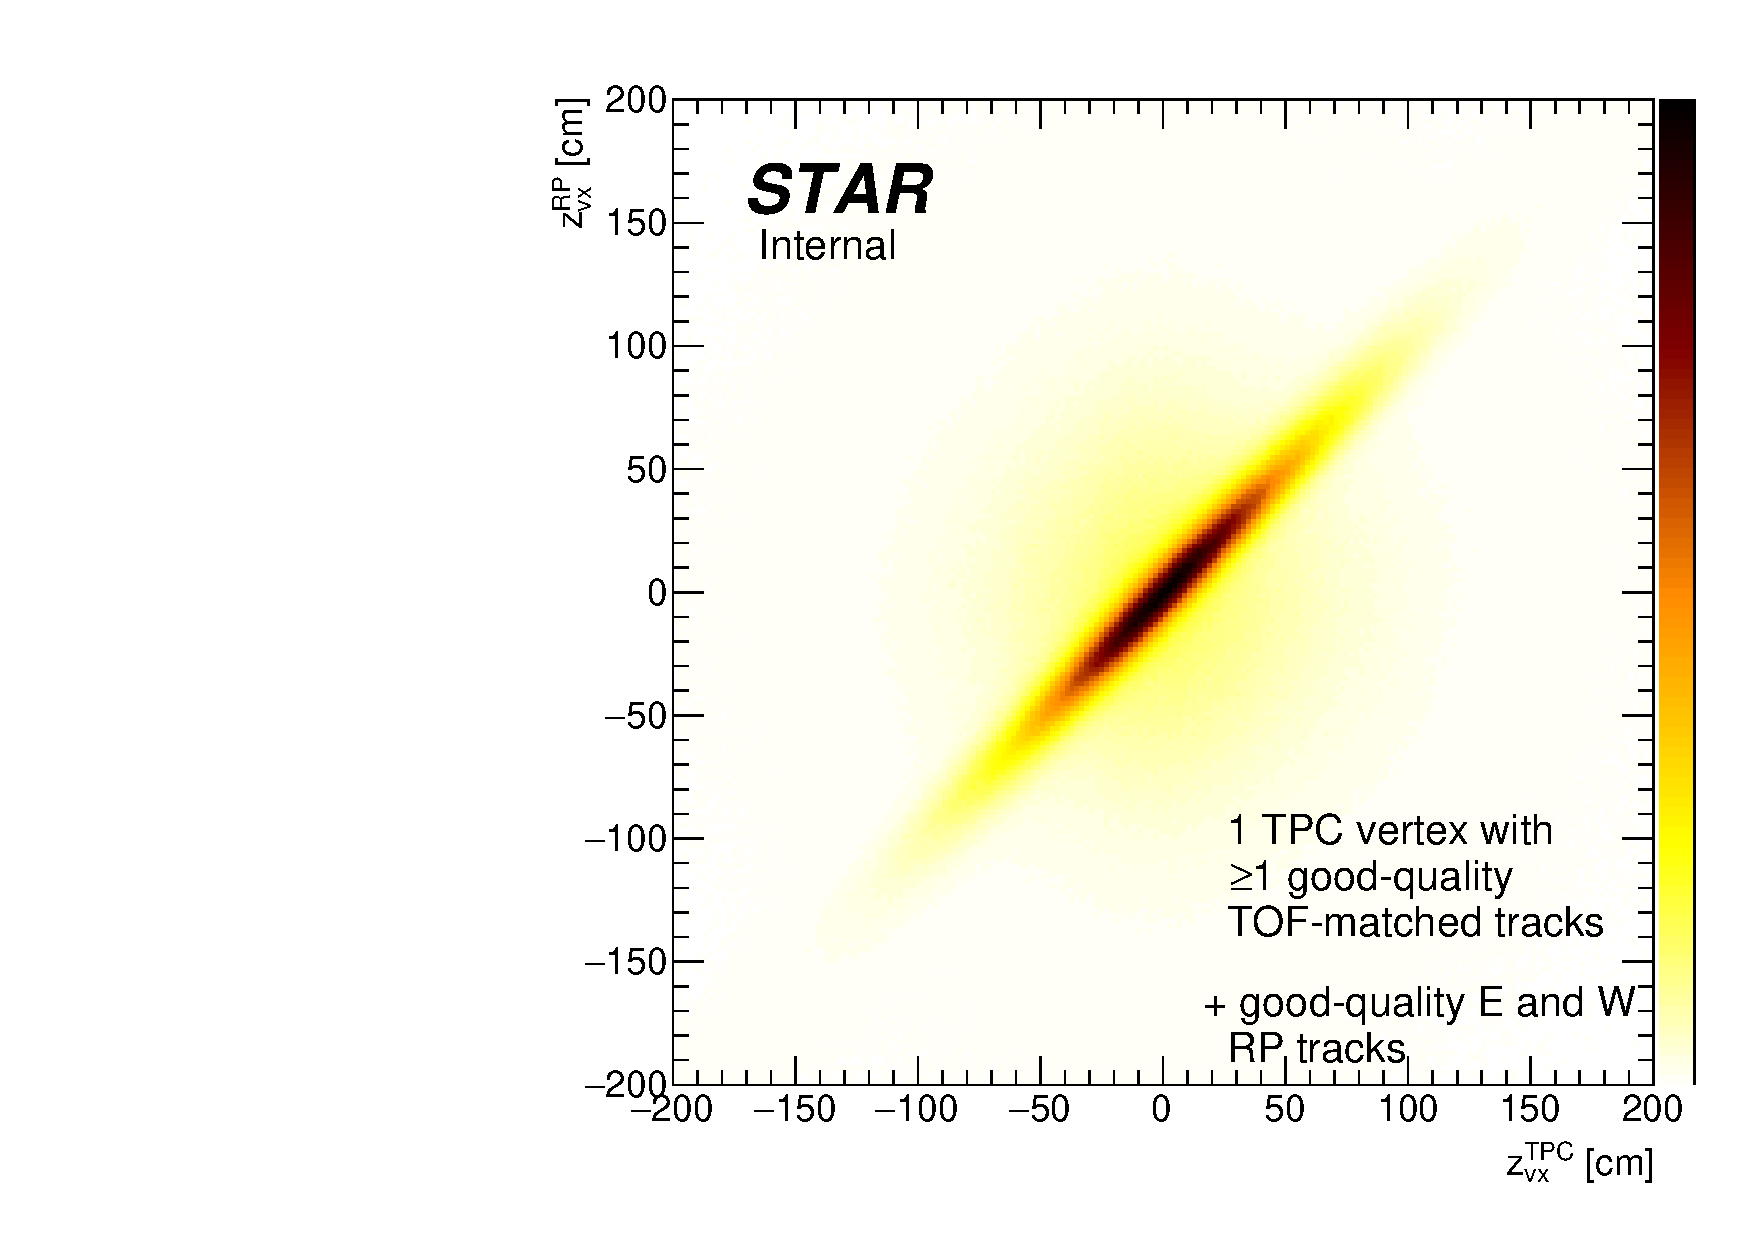
\includegraphics[width=\linewidth]{graphics/eventSelection/zVertexRpVsTpc.pdf}}}
  \end{subfigure}
}
\quad
\parbox{0.545\textwidth}{
  \centering
  \begin{subfigure}[b]{\linewidth}{
                \subcaptionbox{\label{fig:zVertexRpMinusZVertexTpc}}{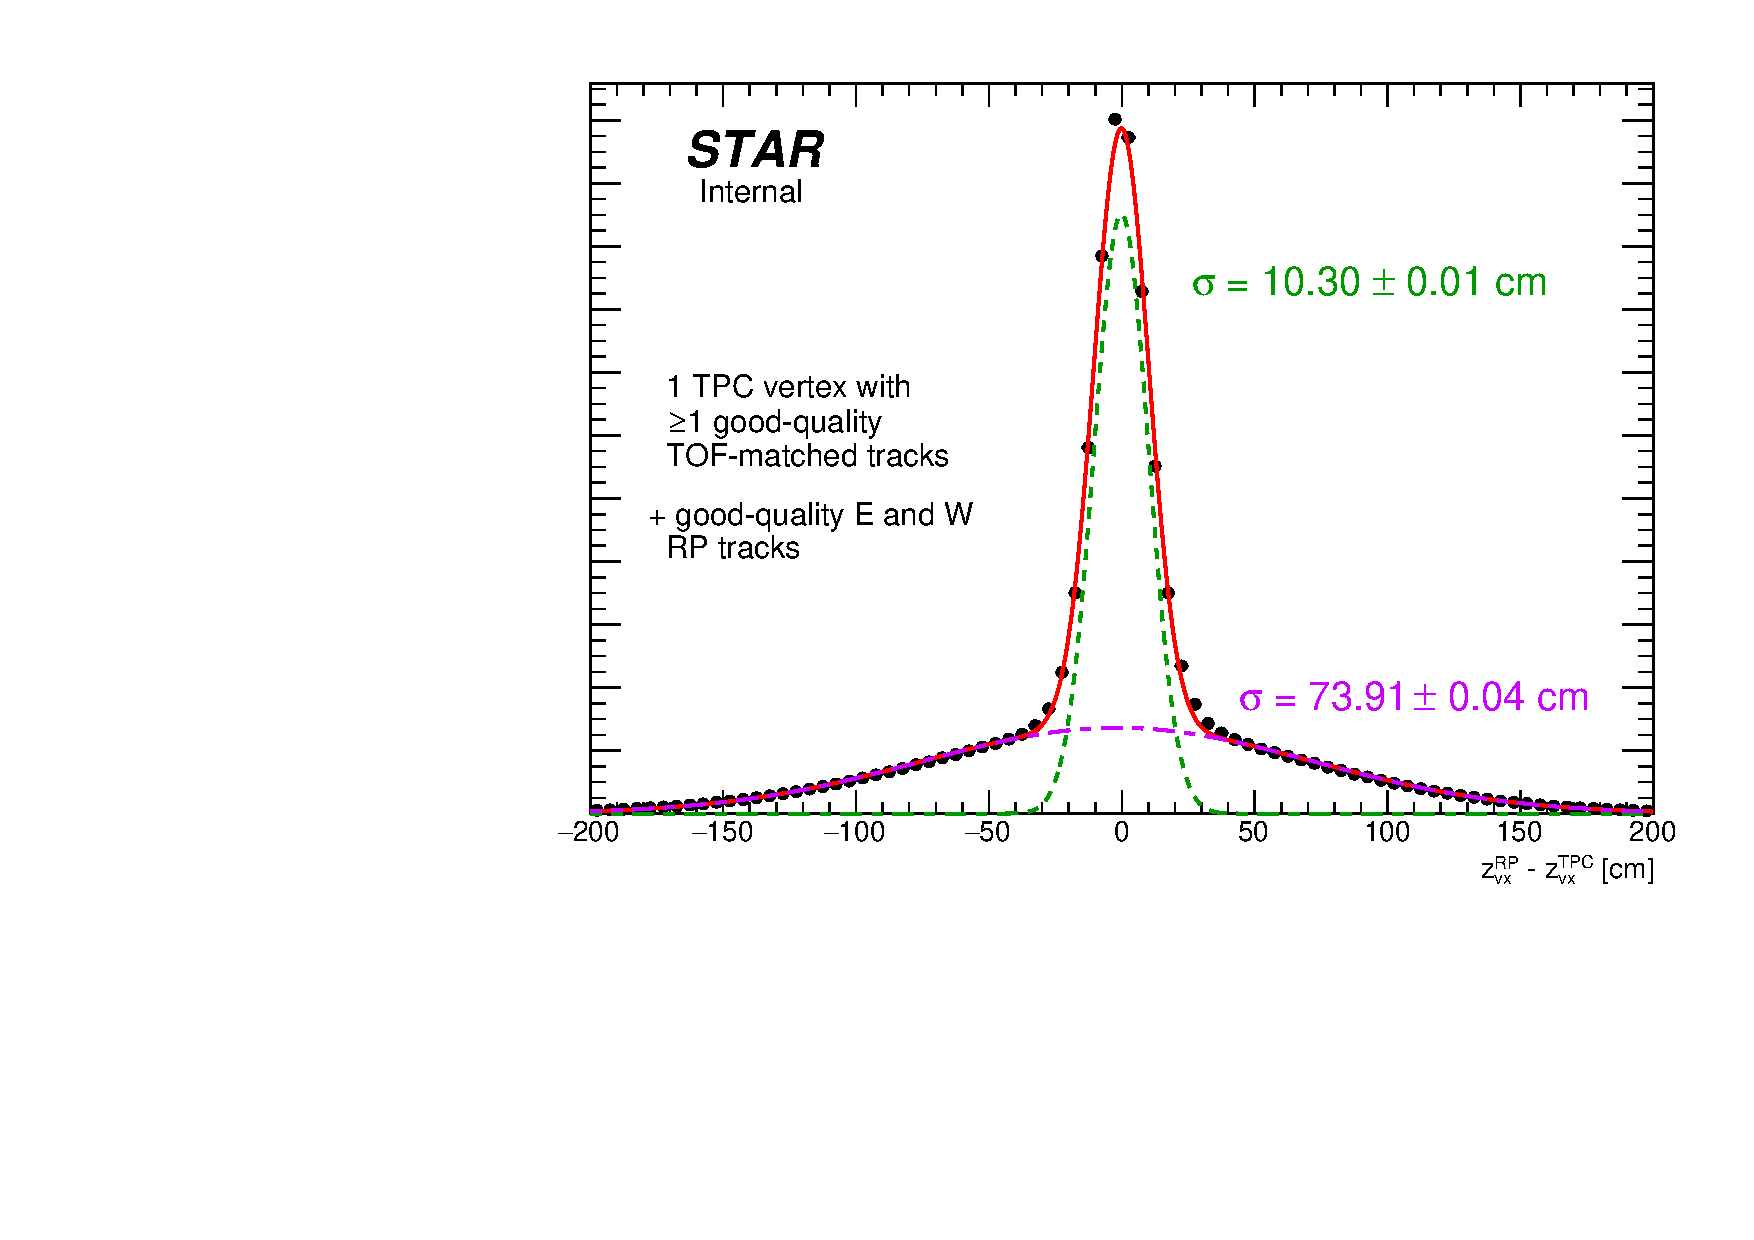
\includegraphics[width=\linewidth]{graphics/eventSelection/zVertexRpMinusZVertexTpc.pdf}}}
  \end{subfigure}
}%
\caption[Correlation and difference of $z$-vertex position measured in Roman Pots and TPC.]{Correlation (Fig.~\ref{fig:zVertexRpVsTpc}) and difference (Fig.~\ref{fig:zVertexRpMinusZVertexTpc}) of $z$-vertex position measured in Roman Pots and TPC in RP\_CPT2 triggers, after preselection described in the plots.}\label{fig:zVertexRpTpc}
\end{figure}%
%---------------------------
The sum of two Gaussian distributions was fitted to data in Fig.~\ref{fig:zVertexRpMinusZVertexTpc} yielding good description of the distribution of $\Delta z_{\text{vtx}}$ with the width parameters equal $10.3$~cm (CD signal) and $73.9$~cm (pile-up). The first parameter reflects the time resolution of RPs (the $z_{\text{vtx}}^{\text{RP}}$ measurement), as the TPC resolution is much better ($\sim 1$~cm). Value of the second parameter, consistent with $\sqrt{2}\sigma_{z_{\text{vtx}}}\approx\sqrt{2}\cdot52~\text{cm}\approx 73.5$~cm, confirms that the wide distribution under the narrow signal peak is uncorrelated background, in other words forward protons originating from a different vertex than the central tracks. To reject this background without significant loss of the signal, we introduce $3.5\sigma_{\Delta z_{\text{vtx}}}$ cut on $\Delta z_{\text{vtx}}$.


% %---------------------------
% \begin{figure}[ht!]
% % \begin{wrapfigure}{l}{0.475\textwidth}%[ht!]
% \centering%
% 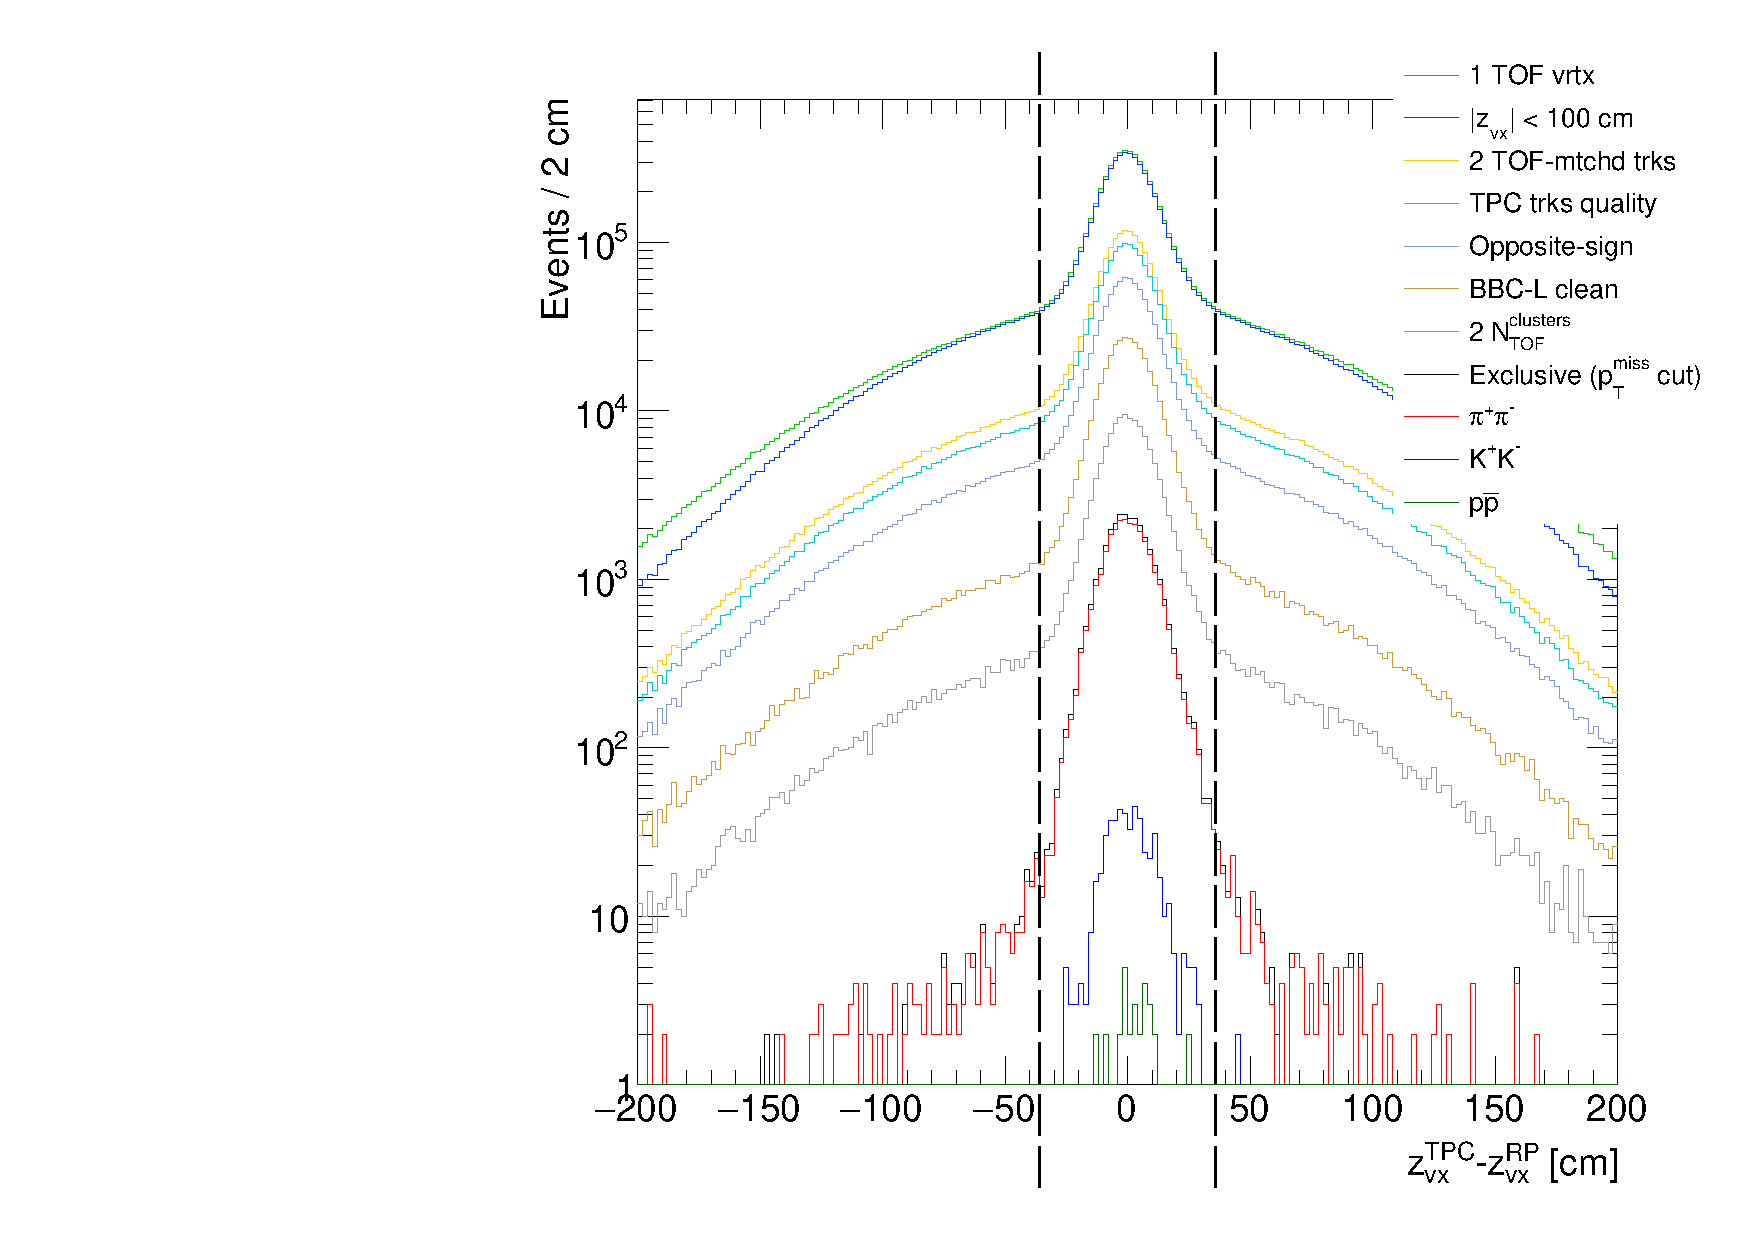
\includegraphics[width=0.475\linewidth,page=1]{graphics/eventSelection/DeltaZVx.pdf}%
% % % 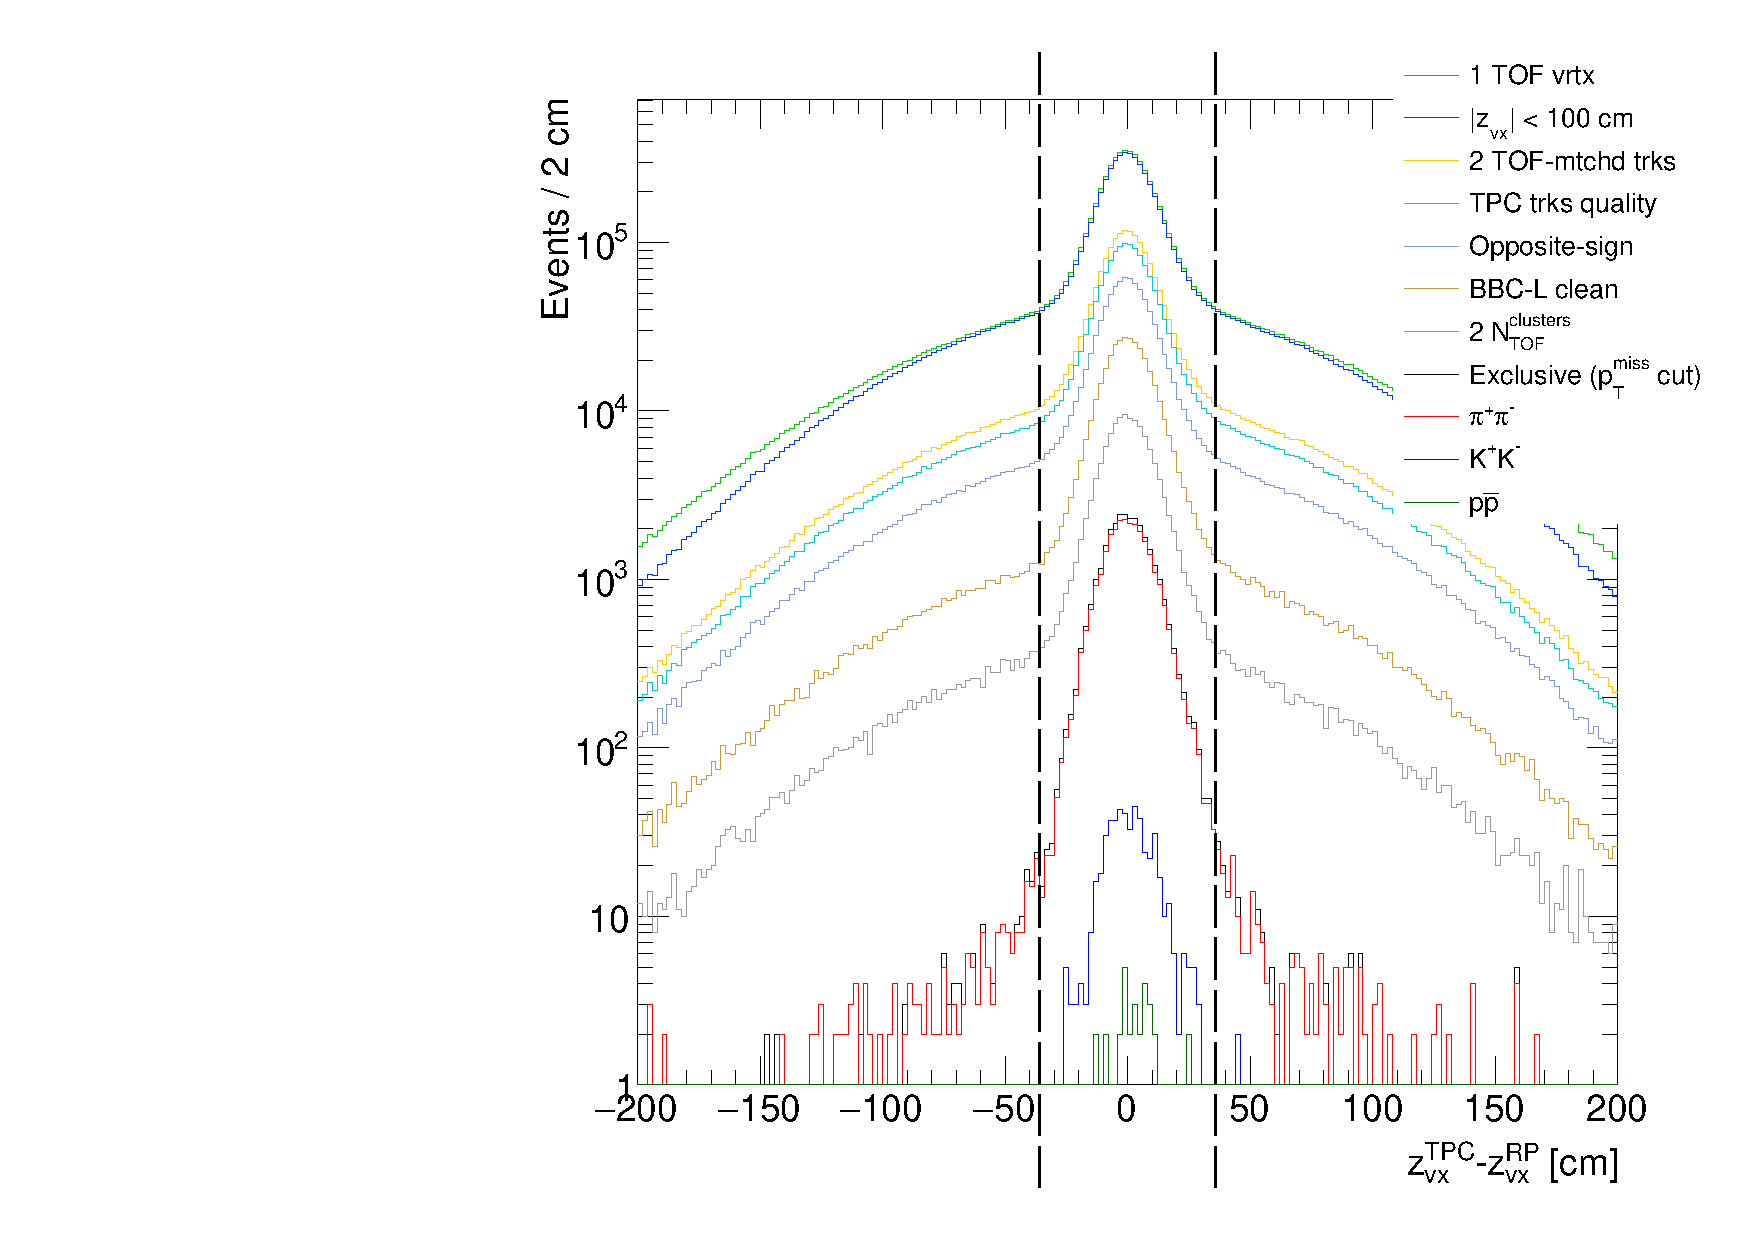
\includegraphics[width=\linewidth,page=1]{graphics/eventSelection/DeltaZVx.pdf}%
% \caption{Delta z-vx.}\label{fig:DeltaZVx}%
% \end{figure}
% % \end{wrapfigure}
% %---------------------------
%%%%%%%%%%%%%%%%%%%%%%%%%%%%%%%%%%%%%%%%%%%%%%%%%%%%%%%%%%%%%%%%%%%%%%%%%%%%%%%%%%%%%%%%%%%%%%%%%%%%%%%%%%%%%%%%%%%%%%%%%%%%%%%%%%%%




%%%%%%%%%%%%%%%%%%%%%%%%%%%%%%%%%%%%%%%%%%%%%%%%%%%%%%%%%%%%%%%%%%%%%%%%%%%%%%%%%%%%%%%%%%%%%%%%%%%%%%%%%%%%%%%%%%%%%%%%%%%%%%%%%%%%
\subsection{(\ref{enum:CutBbcLarge})~BBC-large signal veto}

At the trigger level a veto on signal in small BBC detectors was used. During offline analysis we found that the non-exclusive background can be efficiently rejected if an additional veto on signal in large BBC detectors is added. It is connected with the fact that vast majority of selected RP\_CPT2 triggers were from the central diffraction process to which CEP belongs. Many of central diffraction events have particles produced in the rapidity region outside the TPC and TOF acceptance, some hitting large BBC tiles. Presence of signal in large BBC is therefore a signature of background or a pile-up interaction.

The response of large BBC tiles is different from that of small BBC tiles, as shown in sample plots in Fig.~\ref{fig:sampleBbcResponse} (similar distributions for all channels can be found in Appendix~\ref{appendix:bbc}). Typically in small BBC tiles a peak visible in ADC distribution around $100-150$ (Figs.~\ref{fig:sampleBbcSmallAdcVsTac},\ref{fig:sampleBbcSmallAdc}), a signature of good separation of the electronics noise and signal from the ionizing particle. No such feature is observed in corresponding distribution for large BBC tile (Figs.~\ref{fig:sampleBbcLargeAdcVsTac},\ref{fig:sampleBbcLargeAdc}), which can be explained by the difference in geometry (in size) of small and large tiles. In large BBC tiles the path that scintillation light must travel to reach PMT is much longer in comparison to smal BBC tiles (multiple reflections on the main tile surface due to small thickness of the tile) therefore it is highly attenuated and extended in time. This is possible reason of lack of signal peak in the ADC distribution in large BBC tile spectrum (Fig.~\ref{fig:sampleBbcLargeAdc}), as well as the late-TAC (TAC$<\sim600$, ADC$<100$) tail in the ADC vs. TAC spectrum (slewing effect, Fig.~\ref{fig:sampleBbcLargeAdcVsTac}). Nevertheless, the above features of BBC-large response does not disqualify this detector from being used as a veto detector, as in this case lower efficiency of the detector only reduce the background rejection power.


%---------------------------
\begin{figure}[h]
\centering
\parbox{0.4725\textwidth}{
  \centering
  \begin{subfigure}[b]{\linewidth}
                \subcaptionbox{\label{fig:sampleBbcSmallAdcVsTac}}{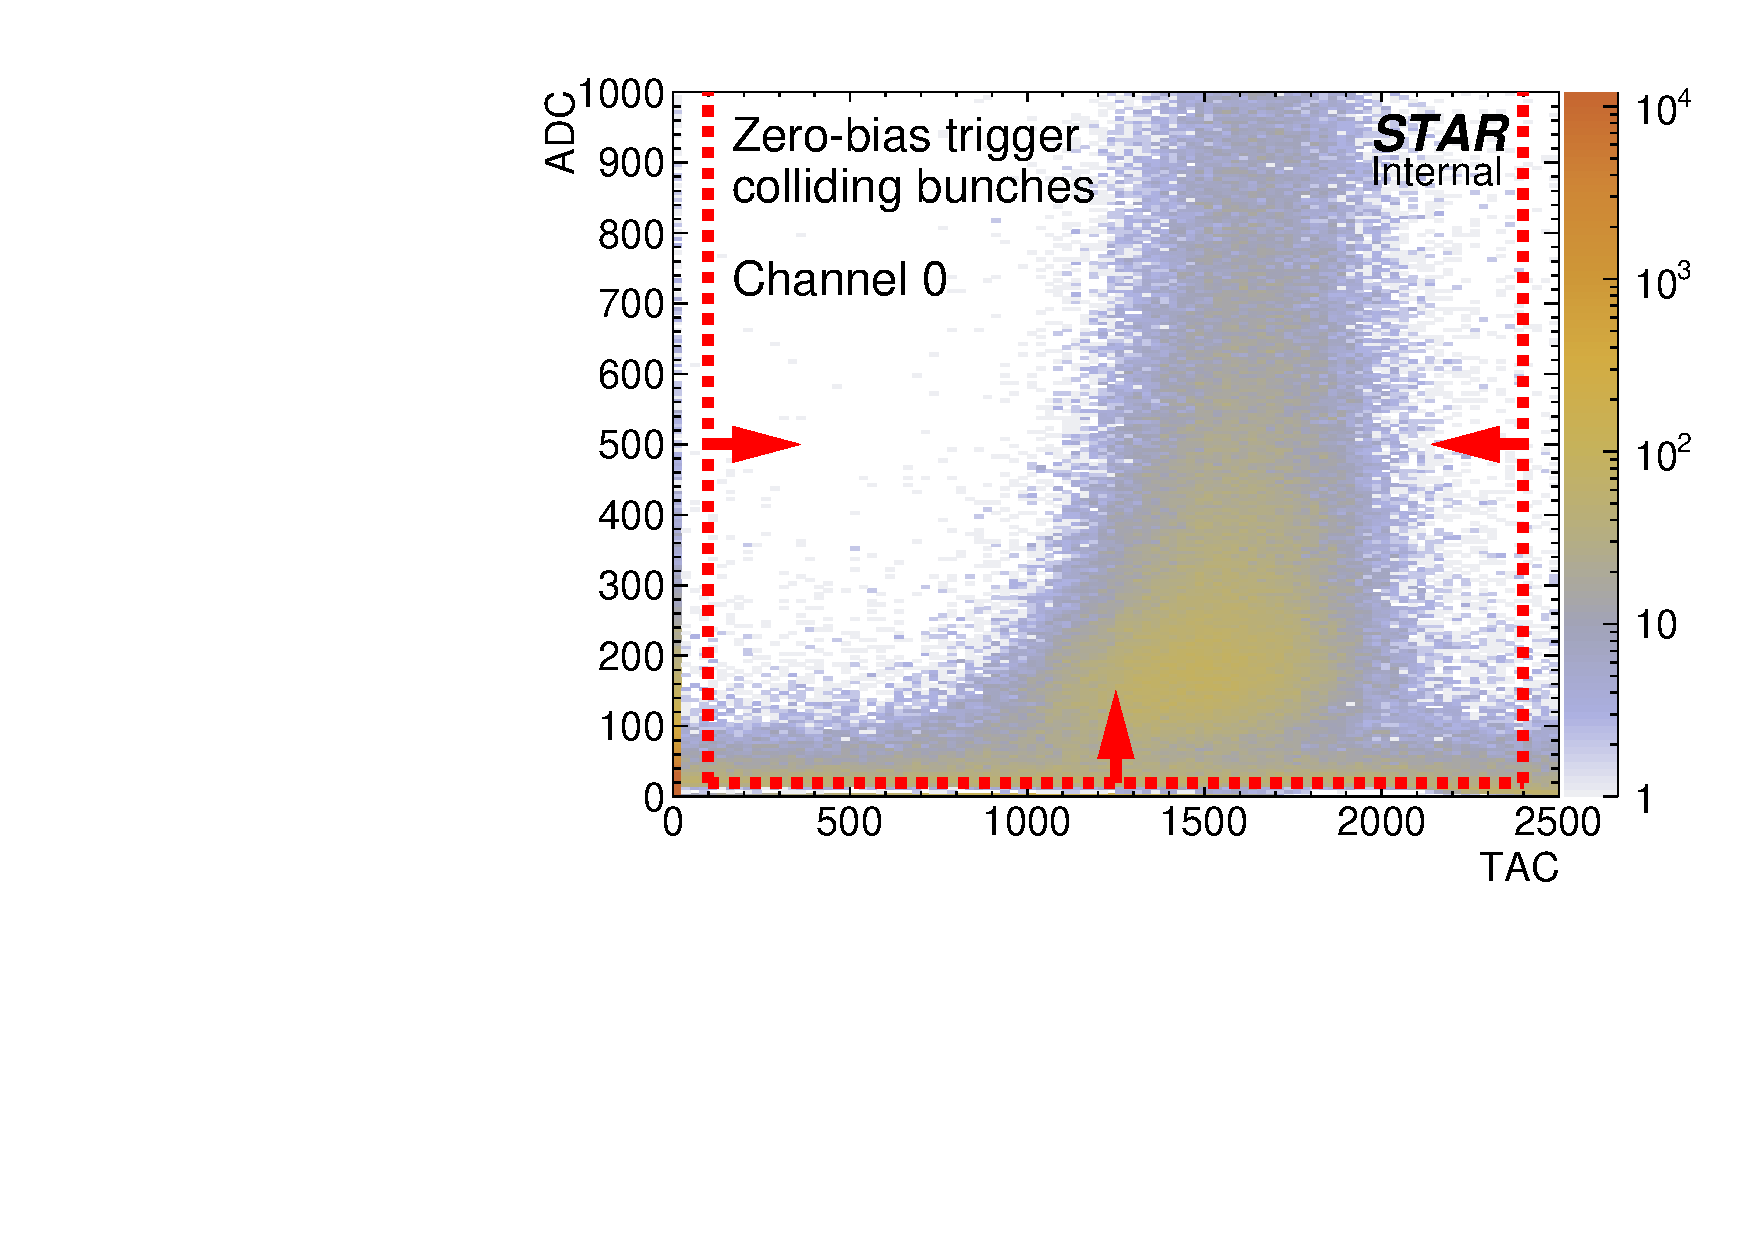
\includegraphics[width=\linewidth,page=1]{graphics/eventSelection/bbc/Bbc_ADCvsTAC_collidingBunches.pdf}}
  \end{subfigure}\\
  \begin{subfigure}[b]{\linewidth}\addtocounter{subfigure}{1}
                \subcaptionbox{\label{fig:sampleBbcSmallAdc}}{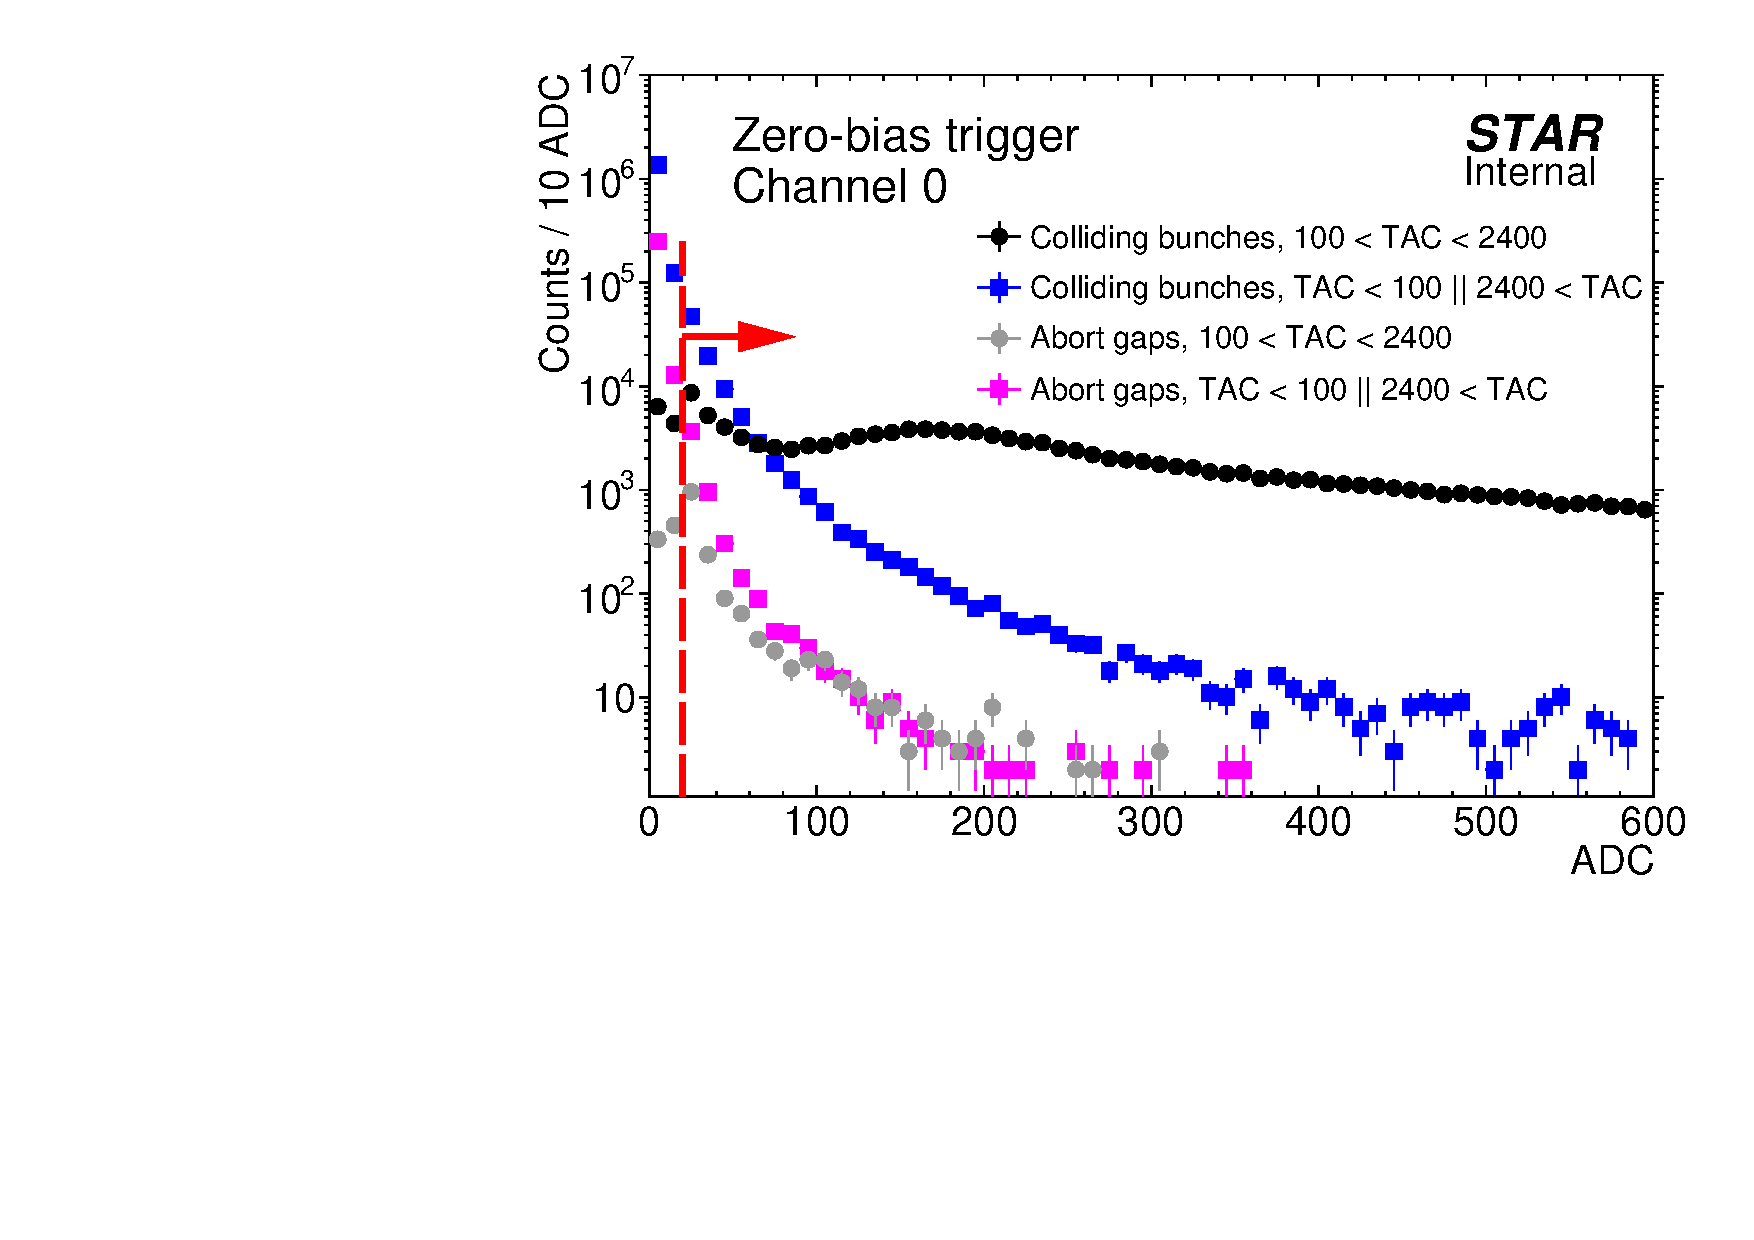
\includegraphics[width=\linewidth,page=1]{graphics/eventSelection/bbc/Bbc_ADC.pdf}}
  \end{subfigure}
}%
\quad\quad%
\parbox{0.4725\textwidth}{
  \centering
  \begin{subfigure}[b]{\linewidth}\addtocounter{subfigure}{-2}
                \subcaptionbox{\label{fig:sampleBbcLargeAdcVsTac}}{\includegraphics[width=\linewidth,page=17]{graphics/eventSelection/bbc/Bbc_ADCvsTAC_collidingBunches.pdf}}
  \end{subfigure}\\
  \begin{subfigure}[b]{\linewidth}\addtocounter{subfigure}{1}
                \subcaptionbox{\label{fig:sampleBbcLargeAdc}}{\includegraphics[width=\linewidth,page=17]{graphics/eventSelection/bbc/Bbc_ADC.pdf}}
  \end{subfigure}
}%
\label{fig:sampleBbcResponse}%
\caption[Sample BBC-small and BBC-large response in zero-bias triggers.]{Sample BBC-small (left column) and BBC-large (right column) response in zero-bias data. Top row shows TAC vs. ADC distributions, bottom row shows projection of the corresponding two-dimensional ditribution on $x$-axis (ADC) in the TAC range quoted in the legend, for both abort gaps and colliding bunches. Red lines and arrows indicate thresholds for a signal in presented channels.}
\end{figure}
%---------------------------


Each channel of the BBC-large has different response to signal from ionizing particle, as well as different level of noise. We decided to set up a signal threshold for each channel based on a study of the noise in abort gaps (in zero-bias data). This noise, in principle, should be solely the electronics noise. We checked for each channel the probability to detect a signal with ADC above certain threshold and with TAC contained within 100 and 2400 (the same window is deafult for small BBC). The result is shown in Fig.~\ref{fig:bbcLargeThresholds}. Next, we established final ADC thresholds in each BBC-large channel by requiring that the noise in BBC-large would cause a veto in maximally $3.5\%$ of events. To transform it to $\text{ADC}_{thr}$ we first assumed that the noise is uncorrelated between the channels. With this assumption one can connect the probability of the veto in whole BBC-large detector (east and west) caused by noise $\mathcal{P}_{\text{veto}}^{\text{noise}}$ with the probability of the signal induced by noise in single BBC-large channel $\mathcal{P}_{i,\text{sig}}^{\text{noise}}$:
\begin{equation}\label{eq:bbcNoise1}
 \mathcal{P}_{\text{veto}}^{\text{noise}} = 1-\mathcal{P}_{!\text{veto}}^{\text{noise}} = 1-\left( 1-\mathcal{P}_{i,\text{sig}}^{\text{noise}} \right)^{N^{\text{BBC}}_{\text{ch}}}.
\end{equation}
In the equation above $N^{\text{BBC}}_{\text{ch}}$ denotes number of active channels in BBC-large. From plots contained in Appendix~\ref{appendix:bbc} one can read that there were 14 active channels in BBC-large. 2 dead channels were found on the west side (40 and 42). By transforming Eq.~\ref{eq:bbcNoise1} to the form presented below we can calculate the threshold probability for a single BBC-large channel:
\begin{equation}\label{eq:bbcNoise2}
 \mathcal{P}_{i,\text{sig}}^{\text{noise}} = 1-\sqrt[N^{\text{BBC}}_{\text{ch}}]{1-\mathcal{P}_{\text{veto}}^{\text{noise}}} = 1-\sqrt[14]{1-0.035} \approx 0.0025.
\end{equation}
In the last step we translated this number to ADC threshold for each channel of BBC-large. For this purpose we used Fig.~\ref{fig:bbcLargeThresholds}. The $x$-axis projection of the crossing point of each color line with the $y$-axis value of 0.0025 defines $\text{ADC}_{thr}$ for each particular channel. These numbers are listed in Tab.~\ref{tab:bbcLargeThresholds}. The event was dropped from analysis if any of the BBC-large channels registered signal of strength $\text{ADC}_{i}>\text{ADC}_{i,thr}$ and $100<\text{TAC}_{i}<2400$.



\begin{table}[h]
	\begin{minipage}{0.65\linewidth}
		\centering
		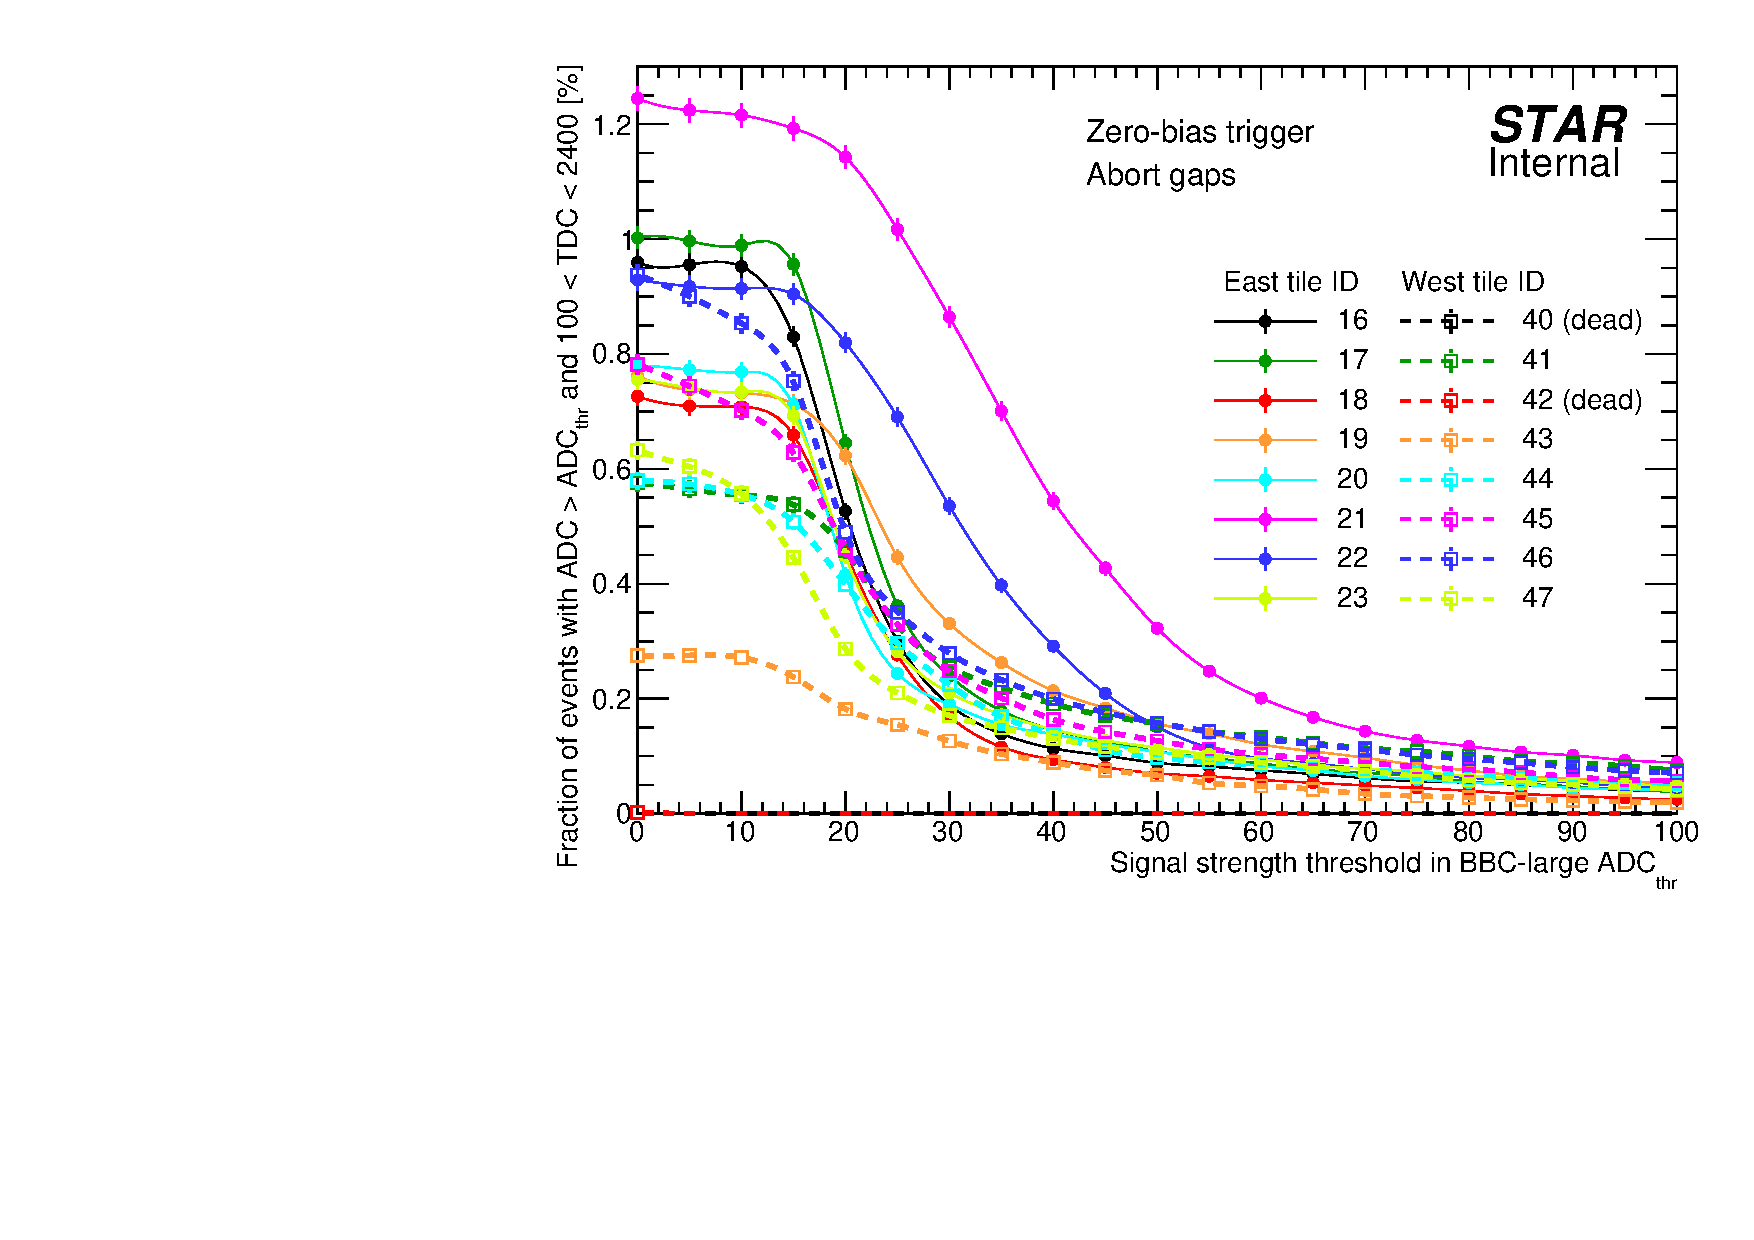
\includegraphics[width=\linewidth]{graphics/eventSelection/bbc/BbbLargeThreshold.pdf}
		\captionof{figure}[Probability of false BBC-large signal (noise-induced).]{Percentage of events in abort gaps from zero-bias triggers with the ADC counts larger than the ADC threshold given in the $x$-axis, for each BBC-large channel. Measured points with statistical uncertainties are connected with a smooth line of corresponding color for better visualization.}
		\label{fig:bbcLargeThresholds}
	\end{minipage}\hfill
	\begin{minipage}{0.3\linewidth}
		\centering
		\begin{tabular}{c|c||c|c}
			\multicolumn{2}{c||}{East} & \multicolumn{2}{c}{West} \\ \hline
			$i$  & $\text{ADC}_{\text{thr}}$ & $i$  & $\text{ADC}_{\text{thr}}$ \\ \hline
			16 & 27 & 40 & 0 \\
			17 & 30 & 41 & 31 \\
			18 & 26 & 42 & 0 \\
			19 & 37 & 43 & 14 \\
			20 & 25 & 44 & 29 \\
			21 & 55 & 45 & 30 \\
			22 & 43 & 46 & 33 \\
			23 & 27 & 47 & 22 \\
		\end{tabular}
		\caption[Offline ADC thresholds in BBC-large.]{Offline ADC thresholds in BBC-large.\newline\newline\newline\newline\newline\newline\newline\newline}
		\label{tab:bbcLargeThresholds}
	\end{minipage}

\end{table}

Observation of high purification of CEP sample with described BBC-large veto in the data from run 15 was helpful to improve the CEP trigger for run 17. The improved trigger called RP\_CPT2noBBCL was similar to RP\_CPT2 with an addition of BBC-large veto using ADC threshold of 50.

%%%%%%%%%%%%%%%%%%%%%%%%%%%%%%%%%%%%%%%%%%%%%%%%%%%%%%%%%%%%%%%%%%%%%%%%%%%%%%%%%%%%%%%%%%%%%%%%%%%%%%%%%%%%%%%%%%%%%%%%%%%%%%%%%%%%



%%%%%%%%%%%%%%%%%%%%%%%%%%%%%%%%%%%%%%%%%%%%%%%%%%%%%%%%%%%%%%%%%%%%%%%%%%%%%%%%%%%%%%%%%%%%%%%%%%%%%%%%%%%%%%%%%%%%%%%%%%%%%%%%%%%%
\subsection{(\ref{enum:CutTofClusters})~TOF clusters limit}

%---------------------------
\begin{figure}[ht!]
% \begin{wrapfigure}{l}{0.475\textwidth}%[ht!]
\centering%
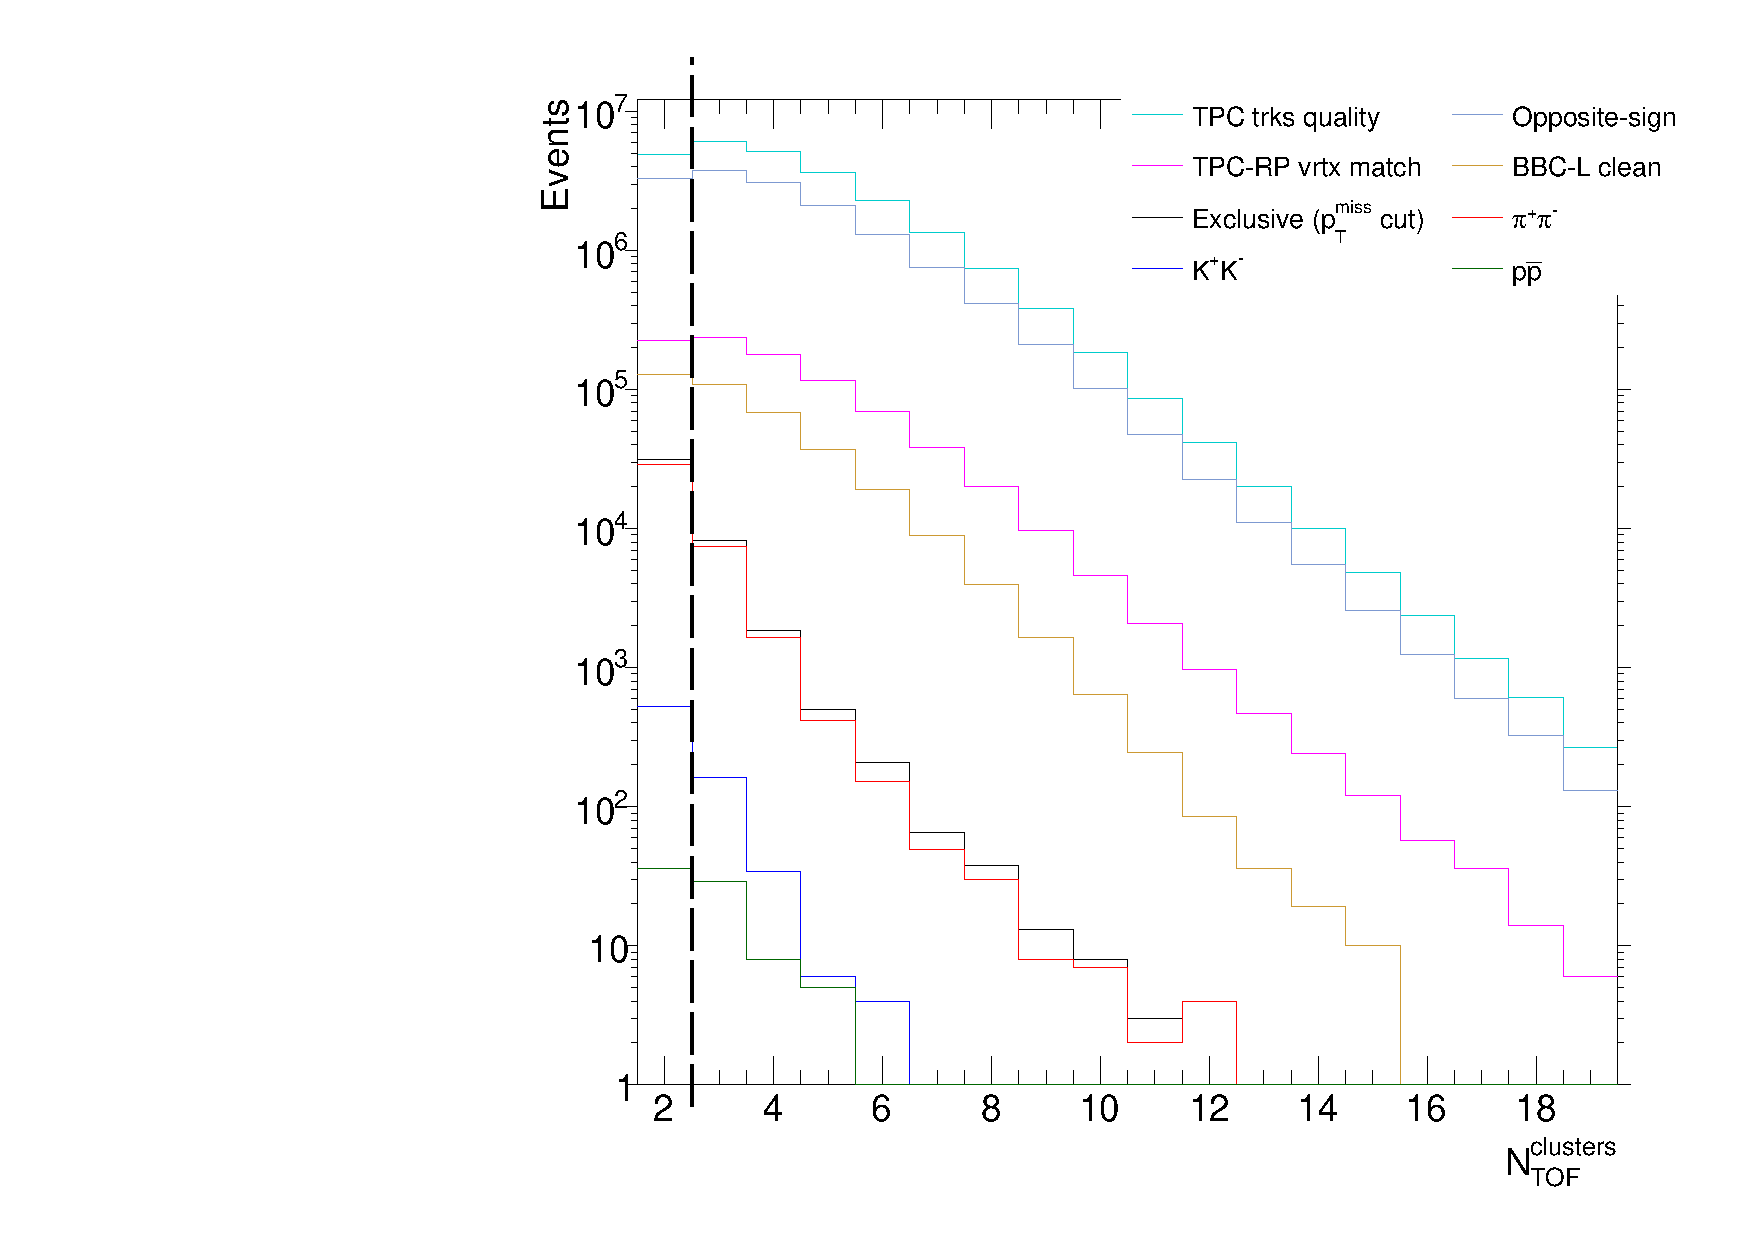
\includegraphics[width=0.475\linewidth,page=1]{graphics/eventSelection/NTofClusters.pdf}%
% % 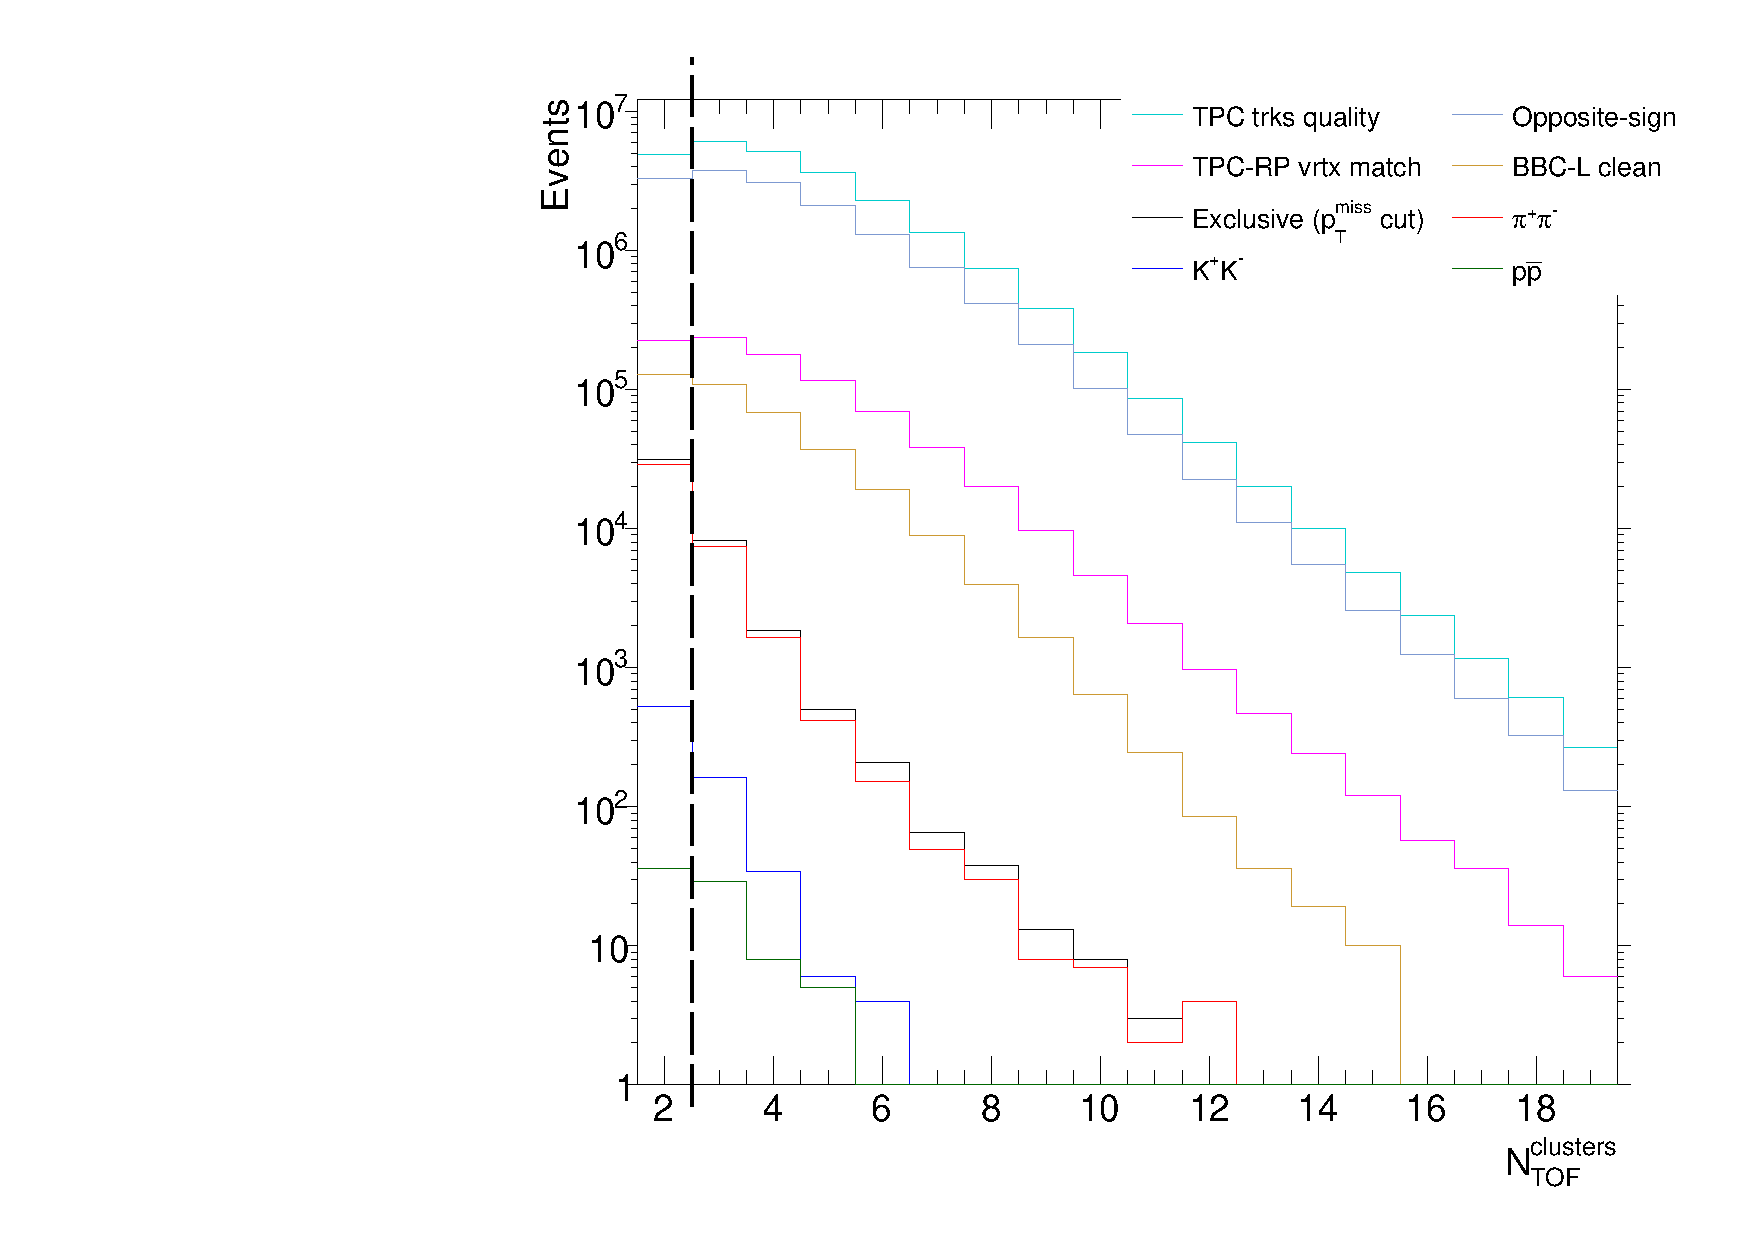
\includegraphics[width=\linewidth,page=1]{graphics/eventSelection/NTofClusters.pdf}% 
\caption{NTofClusters.}\label{fig:NTofClusters}%
\end{figure}
% \end{wrapfigure}
%---------------------------

\subsection{(\ref{enum:CutPid})~Particle identification}\label{subsec:pidCuts}

Particles were identified using combined information from the TPC ($dE/dx$) and TOF (time of hit detection in the TOF subsystem). Merging informations from two sources led to reduction of misidentifications, as well as gave access to higher kaon and proton momentum range where $dE/dx$ of different species overlap.

Compatibility of track $dE/dx$ with that expected from particle of type $X$ was determined using the quantity $n\sigma_{X}$ widely used at STAR, defined as
\protect \begin{equation}\label{eq:nSigmaDef} n\sigma_{X} =  \ln{\left[(dE/dx)^\text{measured} / (dE/dx)_{X}^\text{theory}\right]}~~/~~\sigma_{dE/dx}, \end{equation}
%
where $(dE/dx)^\text{measured}$ is the ionization energy loss of the TPC track, $(dE/dx)_{X}^\text{theory}$ is the Bethe-Bloch~\cite{Bichsel} expectation for the given particle type ($X=\pi$, $K$, $p$) at reconstructed track momentum, and $\sigma_{dE/dx}$ is the statistical uncertainty of $\ln{(dE/dx)^\text{measured}}$. Quantity $n\sigma_{X}$ is in fact a pull: $(dE/dx)^\text{measured}$ is (in first order) an average over $\text{Landau}\otimes\text{normal}$-distributed $dE/dx$ of single TPC hits forming the track, hence according to the central limit theorem\footnote{Keeping in mind that it assumes finite mean and variance of the distribution that summed components follow.} the $(dE/dx)^\text{measured}$ is distributed log-normally and $\ln{(dE/dx)^\text{measured}}$ - normally. From $n\sigma_{X}$ of the two tracks the $\chi^{2}$ statistic for a $XX$ pair hypothesis was calculated:
%
\begin{equation}\label{eq:chiSqDef}\chi^{2}_{dE/dx}(XX) = \left(n\sigma_{X}^{\text{trk1}}\right)^{2} + \left(n\sigma_{X}^{\text{trk2}}\right)^{2}.\end{equation}
%
Sometimes we also quote $n\sigma^{\text{pair}}$ quantity (which is no longer a Gaussian pull) connected with $\chi^{2}$ through relation
%
\begin{equation}\label{eq:nSigmaPairDef}n\sigma^{\text{pair}}_{X} = \sqrt{\chi^{2}_{dE/dx}(XX)} = \sqrt{\left(n\sigma_{X}^{\text{trk1}}\right)^{2} + \left(n\sigma_{X}^{\text{trk2}}\right)^{2}}.\end{equation}
%
The time of detection of particle in the TOF system was used to reconstruct its squared mass $m^{2}_{\text{TOF}}$. For this purpose the time of primary interaction is typically used (''start time``), reconstructed by detecting fragments of dissociated beam particles in VPD detectors on both sides of the interaction point\footnote{Time measured from protons in the RP detectors cannot be used because RP readout runs on independent clock from that used by VPD and TOF.}. However, it is not accessible in CEP as the initial protons survive the interaction intact. We therefore assumed that both central tracks are of the same type which is natural consequence of quantum number conservation. With this assumption the time difference between TOF hits and measured tracks' momenta and lengths of helical paths between the primary vertex and TOF then allow to calculate $m^{2}_{\text{TOF}}$. The derivation of formula used to obtain $m^{2}_{\text{TOF}}$ is presented in Appendix~\ref{appendix:squaredMass}.

Particle identification involved a few steps. First, the $pp$ hypothesis was verified:
\begin{equation}\label{eq:pidPPbar}\lefteqn{\overbrace{\phantom{\chi^{2}_{dE/dx}(pp)<9\;\;\; \& \;\;\; m^{2}_{\text{TOF}} > 0.6~\mbox{GeV}^{2}}}^{\text{likely}~pp}}\chi^{2}_{dE/dx}(pp)<9\;\;\; \& \;\;\; \underbrace{m^{2}_{\text{TOF}} > 0.6~\mbox{GeV}^{2}\;\;\; \& \;\;\; \chi^{2}_{dE/dx}(\pi\pi)>9\;\;\; \& \;\;\; \chi^{2}_{dE/dx}(KK)>9}_{\text{unlikely}~\pi\pi~\text{or}~KK}.\end{equation}
If any of above was not satisfied, the pair was checked for compatibility with $KK$ hypothesis:
%
\begin{equation}\label{eq:pidKK}%
\lefteqn{\overbrace{\phantom{\chi^{2}_{dE/dx}(KK)<9\;\;\; \& \;\;\; m^{2}_{\text{TOF}} > 0.15~\mbox{GeV}^{2}}}^{\text{likely}~KK}}\chi^{2}_{dE/dx}(KK)<9\;\;\; \& \;\;\; \underbrace{m^{2}_{\text{TOF}} > 0.15~\mbox{GeV}^{2}\;\;\; \& \;\;\; \chi^{2}_{dE/dx}(\pi\pi)>9}_{\text{unlikely}~\pi\pi}\;\;\; \& \;\;\; \underbrace{\chi^{2}_{dE/dx}(pp)>9}_{\text{unlikely}~pp}.
\end{equation}
%
In case the pair was neither recognized as $p\bar{p}$ or $K^{+}K^{-}$, it was assumed to be a $\pi^{+}\pi^{-}$ pair if the $dE/dx$ of positive and negative charge track was consistent with pion hypothesis at $3\sigma$ level:
\begin{equation}\label{eq:pidPiPi}|n\sigma_{\pi}^{\text{trk1}}|<3\;\;\; \& \;\;\; |n\sigma_{\pi}^{\text{trk2}}|<3.\end{equation}




\begin{figure}[h]
\centering
\parbox{0.4725\textwidth}{
  \centering
  \begin{subfigure}[b]{\linewidth}
                \subcaptionbox{\label{fig:SqRootNSigma2D_a}}{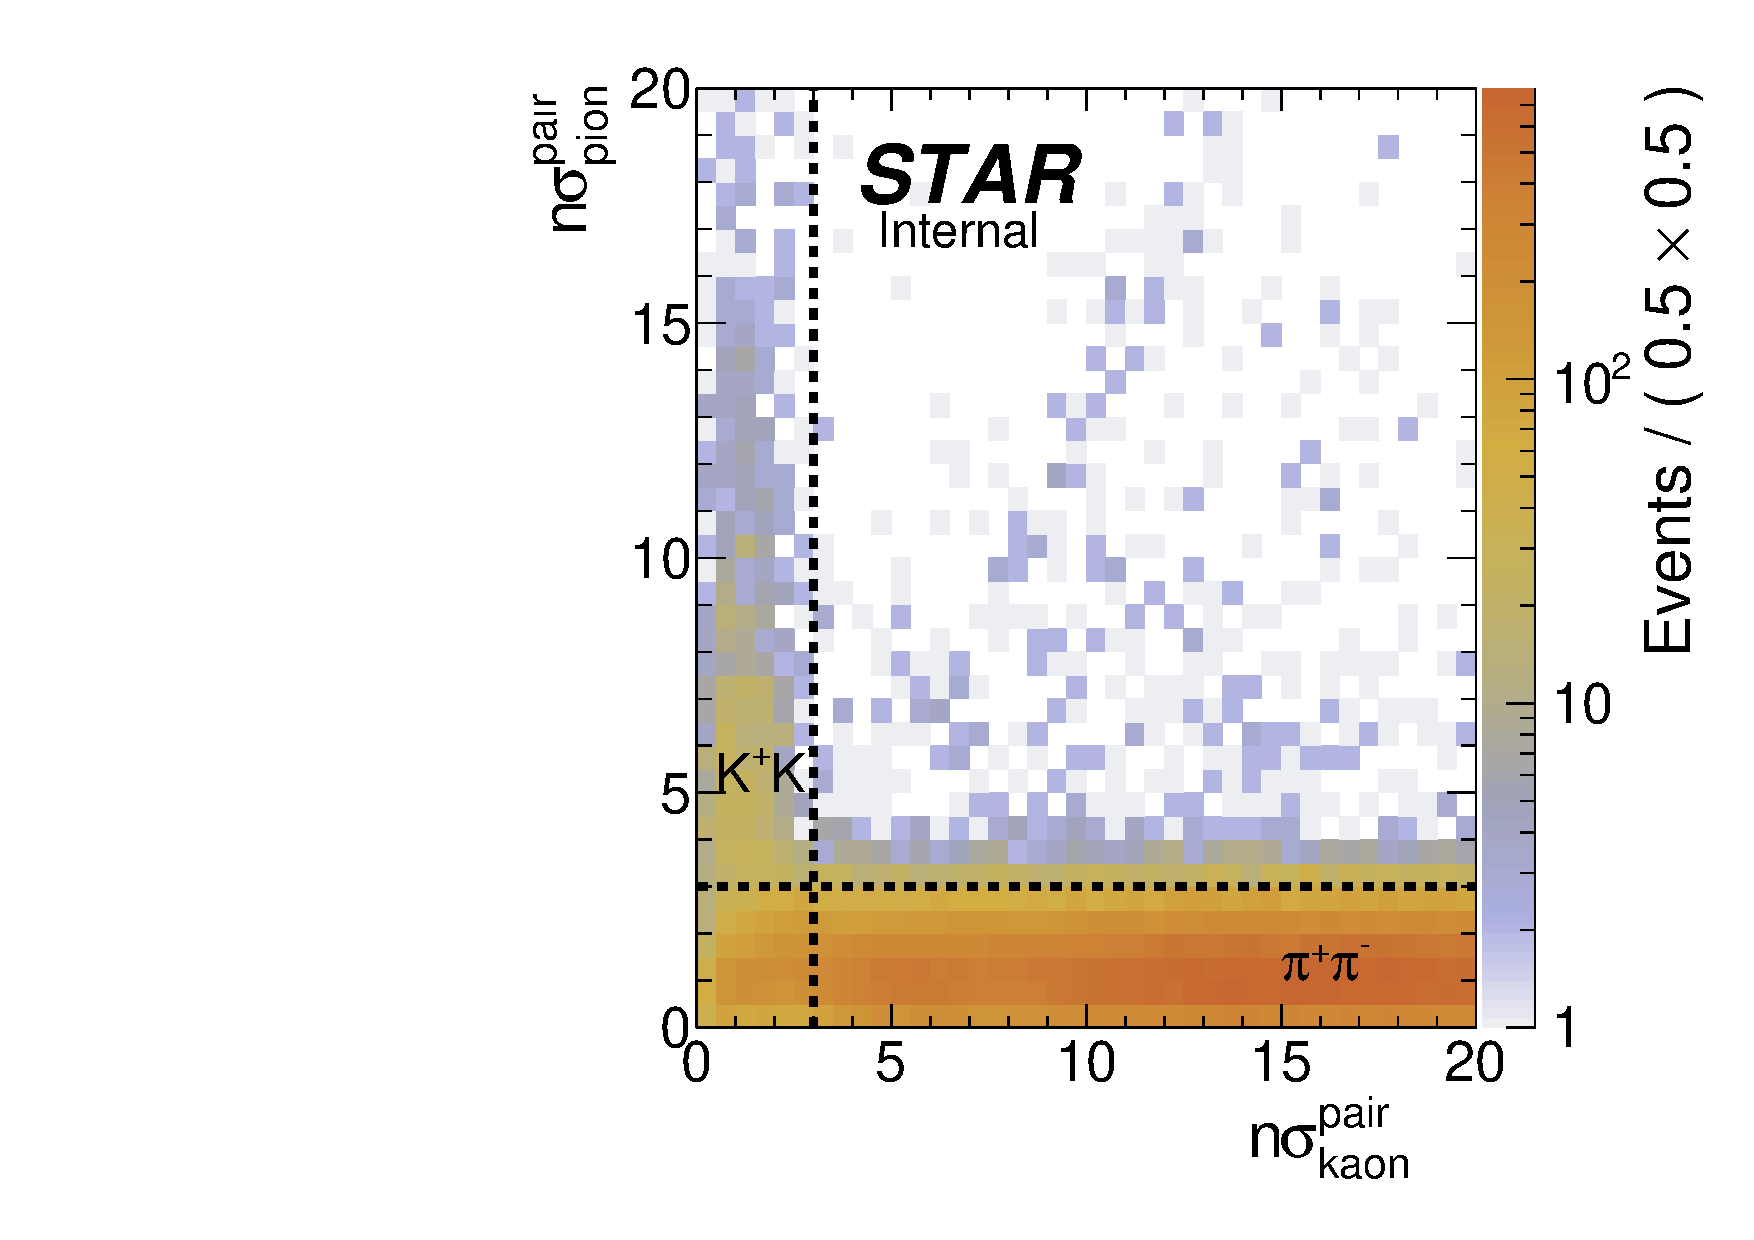
\includegraphics[width=1.05\linewidth,page=1]{graphics/eventSelection/pid/PidSelector_SqRootNSigma2D.pdf}}
  \end{subfigure}\\
  \begin{subfigure}[b]{\linewidth}\addtocounter{subfigure}{1}
                \subcaptionbox{\label{fig:SqRootNSigma2D_c}}{\includegraphics[width=1.05\linewidth,page=3]{graphics/eventSelection/pid/PidSelector_SqRootNSigma2D.pdf}}
  \end{subfigure}
}%
\quad\quad%
\parbox{0.4725\textwidth}{
  \centering
  \begin{subfigure}[b]{\linewidth}\addtocounter{subfigure}{-2}\vspace*{-13pt}
                \subcaptionbox{\label{fig:SqRootNSigma2D_b}}{\includegraphics[width=1.05\linewidth,page=2]{graphics/eventSelection/pid/PidSelector_SqRootNSigma2D.pdf}}
  \end{subfigure}\\
  \begin{minipage}[t][1.042\linewidth][t]{\linewidth}\vspace{10pt}
    \caption[$n\sigma^{\text{pair}}_{X}$ vs. $n\sigma^{\text{pair}}_{Y}$.]{Two-dimensional distributions of $n\sigma^{\text{pair}}_{\pi}$ vs.~$n\sigma^{\text{pair}}_{K}$ (\ref{fig:SqRootNSigma2D_a}), $n\sigma^{\text{pair}}_{\pi}$ vs.~$n\sigma^{\text{pair}}_{p}$ and $n\sigma^{\text{pair}}_{K}$ vs.~$n\sigma^{\text{pair}}_{p}$ for exclusive event candidates after full event selection except PID cuts (except cuts~\ref{enum:CutPid}). Dashed lines indicate the value of $n\sigma^{\text{pair}}$ which is used in pair identification~\ref{enum:CutPid} ($n\sigma^{\text{pair}}_{X}=9$ which is equivalent to $\chi^{2}(XX)=9$).}\label{fig:SqRootNSigma2D}
  \end{minipage}
}%

\end{figure}
%--------------------------- 


In Fig.~\ref{fig:SqRootNSigma2D} we present two-dimensional distributions of $n\sigma^{\text{pair}}$ variables which help better undestand the behaviour and aim of $n\sigma^{\text{pair}}$ ($\chi^{2}$) cuts in Eqs.~\eqref{eq:pidPPbar}, \eqref{eq:pidKK}. Regions of enriched population of specific pair species are appropriately labeled. Similar connections between $n\sigma^{\text{pair}}$ and $m^{2}_{\text{TOF}}$ are shown in Fig.~\ref{fig:mSqVsNSigmaPair}.
 


% %--------------------------- 
% \begin{figure}[ht!]
% \centering 
% \parbox{0.315\textwidth}{
%   \centering
%   \begin{subfigure}[b]{\linewidth}{
%                 \subcaptionbox{\label{fig:SqRootNSigmaPionVsKaon}}{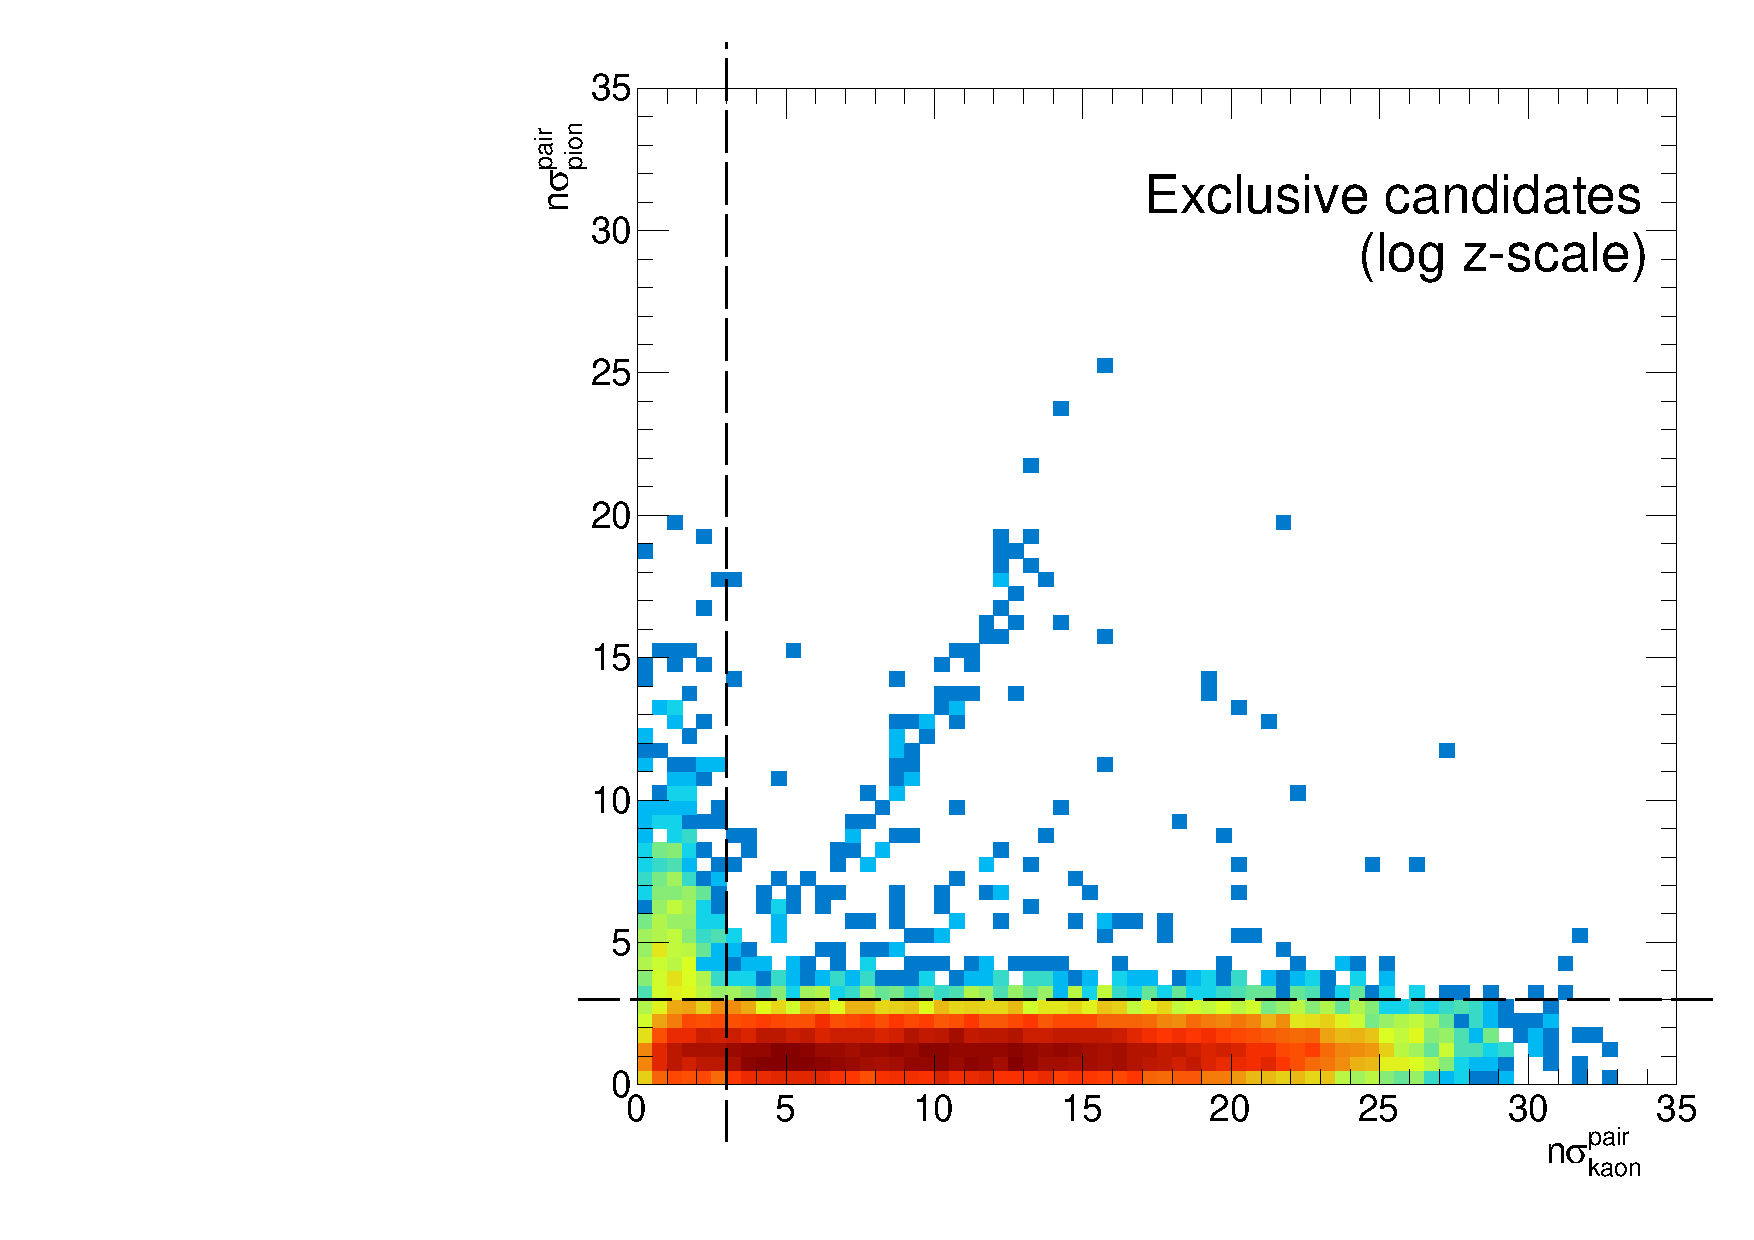
\includegraphics[width=\linewidth]{graphics/eventSelection/SqRootNSigmaPionVsKaon.pdf}}}
%   \end{subfigure}
% }
% \quad
% \parbox{0.315\textwidth}{
%   \centering
%   \begin{subfigure}[b]{\linewidth}{
%                 \subcaptionbox{\label{fig:SqRootNSigmaPionVsProton}}{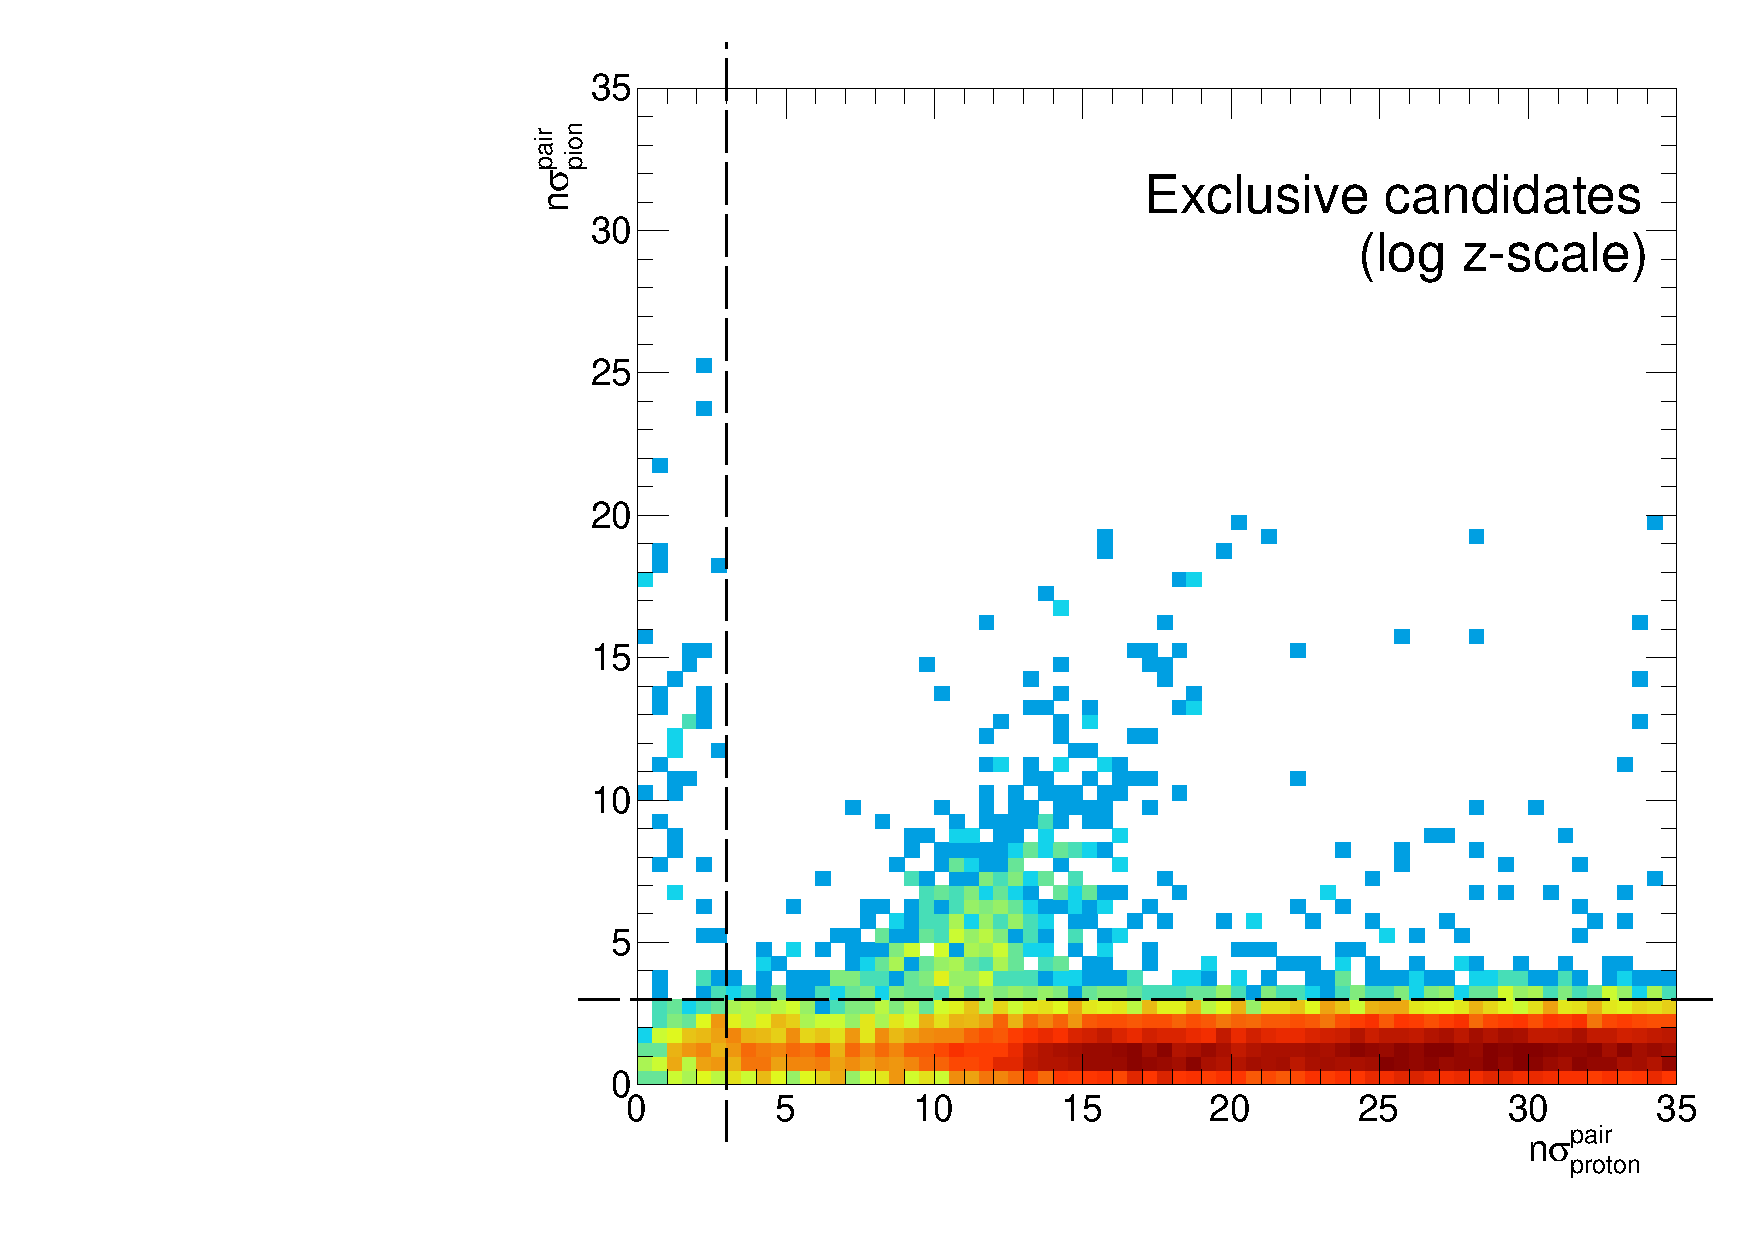
\includegraphics[width=\linewidth]{graphics/eventSelection/SqRootNSigmaPionVsProton.pdf}}}
%   \end{subfigure}
% }
% \quad
% \parbox{0.315\textwidth}{
%   \centering
%   \begin{subfigure}[b]{\linewidth}{
%                 \subcaptionbox{\label{fig:SqRootNSigmaKaonVsProton}}{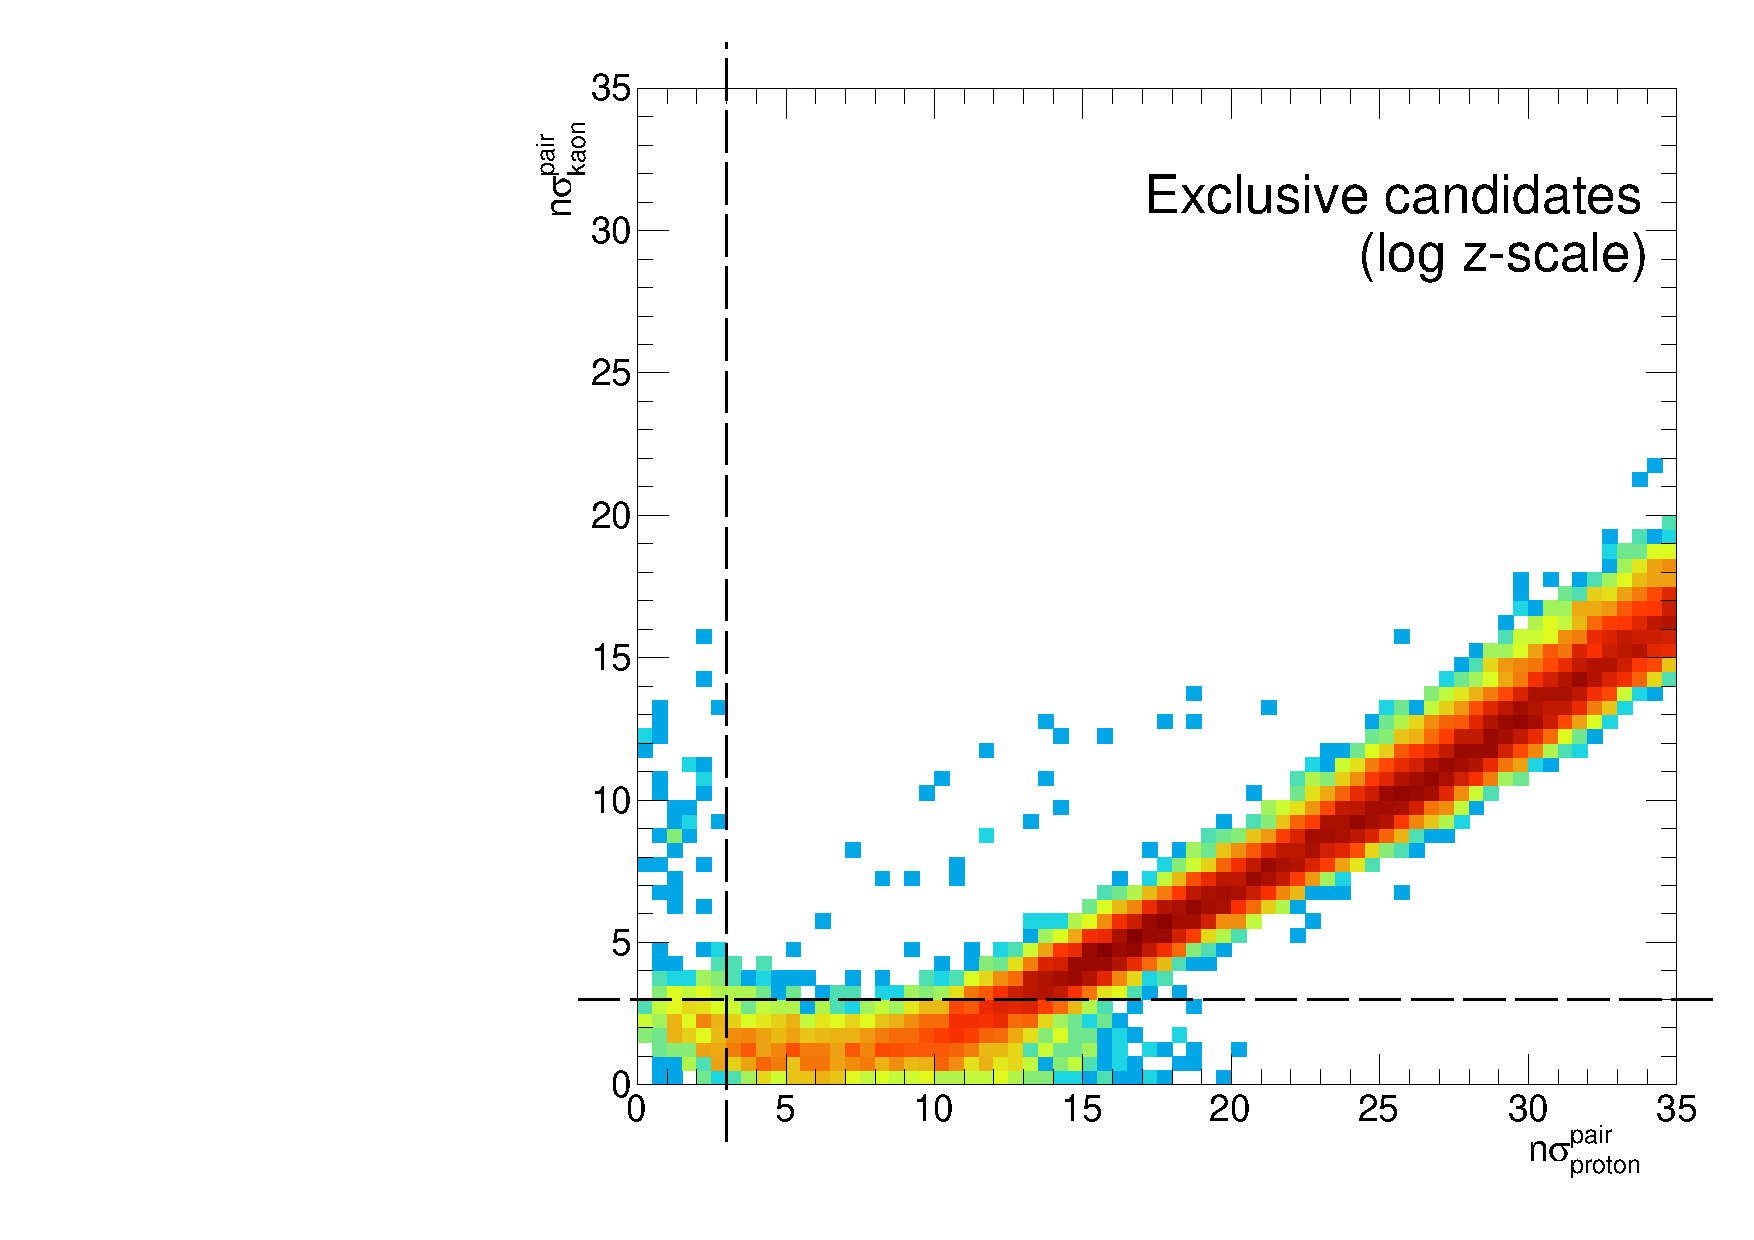
\includegraphics[width=\linewidth]{graphics/eventSelection/SqRootNSigmaKaonVsProton.pdf}}}
%   \end{subfigure}
% }%
% \caption{Correlation between $n\sigma^{\text{pair}}$ from TPC for $\pi^{+}\pi^{-}$, $K^{+}K^{-}$ and $p\bar{p}$.} 
% \end{figure}
% %---------------------------
% 
% 
 
\begin{figure}[ht!]
  \centering
  \begin{tabular}{@{}p{0.47\linewidth}@{\quad\quad}p{0.47\linewidth}@{}}
    \subfigimg[width=\linewidth,page=1]{~~~~~~~~~~~a)}{graphics/eventSelection/pid/PidSelector_SqMassTofVsSqRootNSigma_pion.pdf} &
    \subfigimg[width=\linewidth,page=1]{~~~~~~~~~~~c)}{graphics/eventSelection/pid/SqMassTofVsSqRootNSigma_pion.pdf} \\[-10pt]
    \subfigimg[width=\linewidth,page=1]{~~~~~~~~~~~d)}{graphics/eventSelection/pid/PidSelector_SqMassTofVsSqRootNSigma_kaon.pdf} &
    \subfigimg[width=\linewidth,page=1]{~~~~~~~~~~~f)}{graphics/eventSelection/pid/SqMassTofVsSqRootNSigma_kaon.pdf} \\[-10pt]
    \subfigimg[width=\linewidth,page=1]{~~~~~~~~~~~g)}{graphics/eventSelection/pid/PidSelector_SqMassTofVsSqRootNSigma_proton.pdf} &
    \subfigimg[width=\linewidth,page=1]{~~~~~~~~~~~i)}{graphics/eventSelection/pid/SqMassTofVsSqRootNSigma_proton.pdf}    
  \end{tabular}\vspace*{-5pt}
  \caption[$n\sigma^{\text{pair}}_{X}$ vs. $m^{2}_{\text{TOF}}$.]{Two-dimensional distributions of $n\sigma^{\text{pair}}_{\pi}$ (top row), $n\sigma^{\text{pair}}_{K}$ (middle row) and $n\sigma^{\text{pair}}_{p}$ (bottom row) vs. $m^{2}_{\text{TOF}}$. The left column contains all clean BBC-large events with single TOF vertex and two opposite sign TOF-matched tracks (passing cuts~\ref{enum:CutPrimVx}, \ref{enum:TpcTofMatched}, \ref{enum:TpcOppoSign} and~\ref{enum:CutBbcLarge}), which provides excellent statistics to see the signatures or pairs of specific ID. The right column cantains exclusive event candidates after full event selection except PID cuts (except cuts~\ref{enum:CutPid}). Dashed red line and arrow indicate the cut imposed on plotted quantities which are used to select exclusive pairs of given particle species (keep in mind that these are not the only cuts).}\label{fig:mSqVsNSigmaPair}
\end{figure}






%%%%%%%%


% \begin{figure}[tbp]
% \centering
% 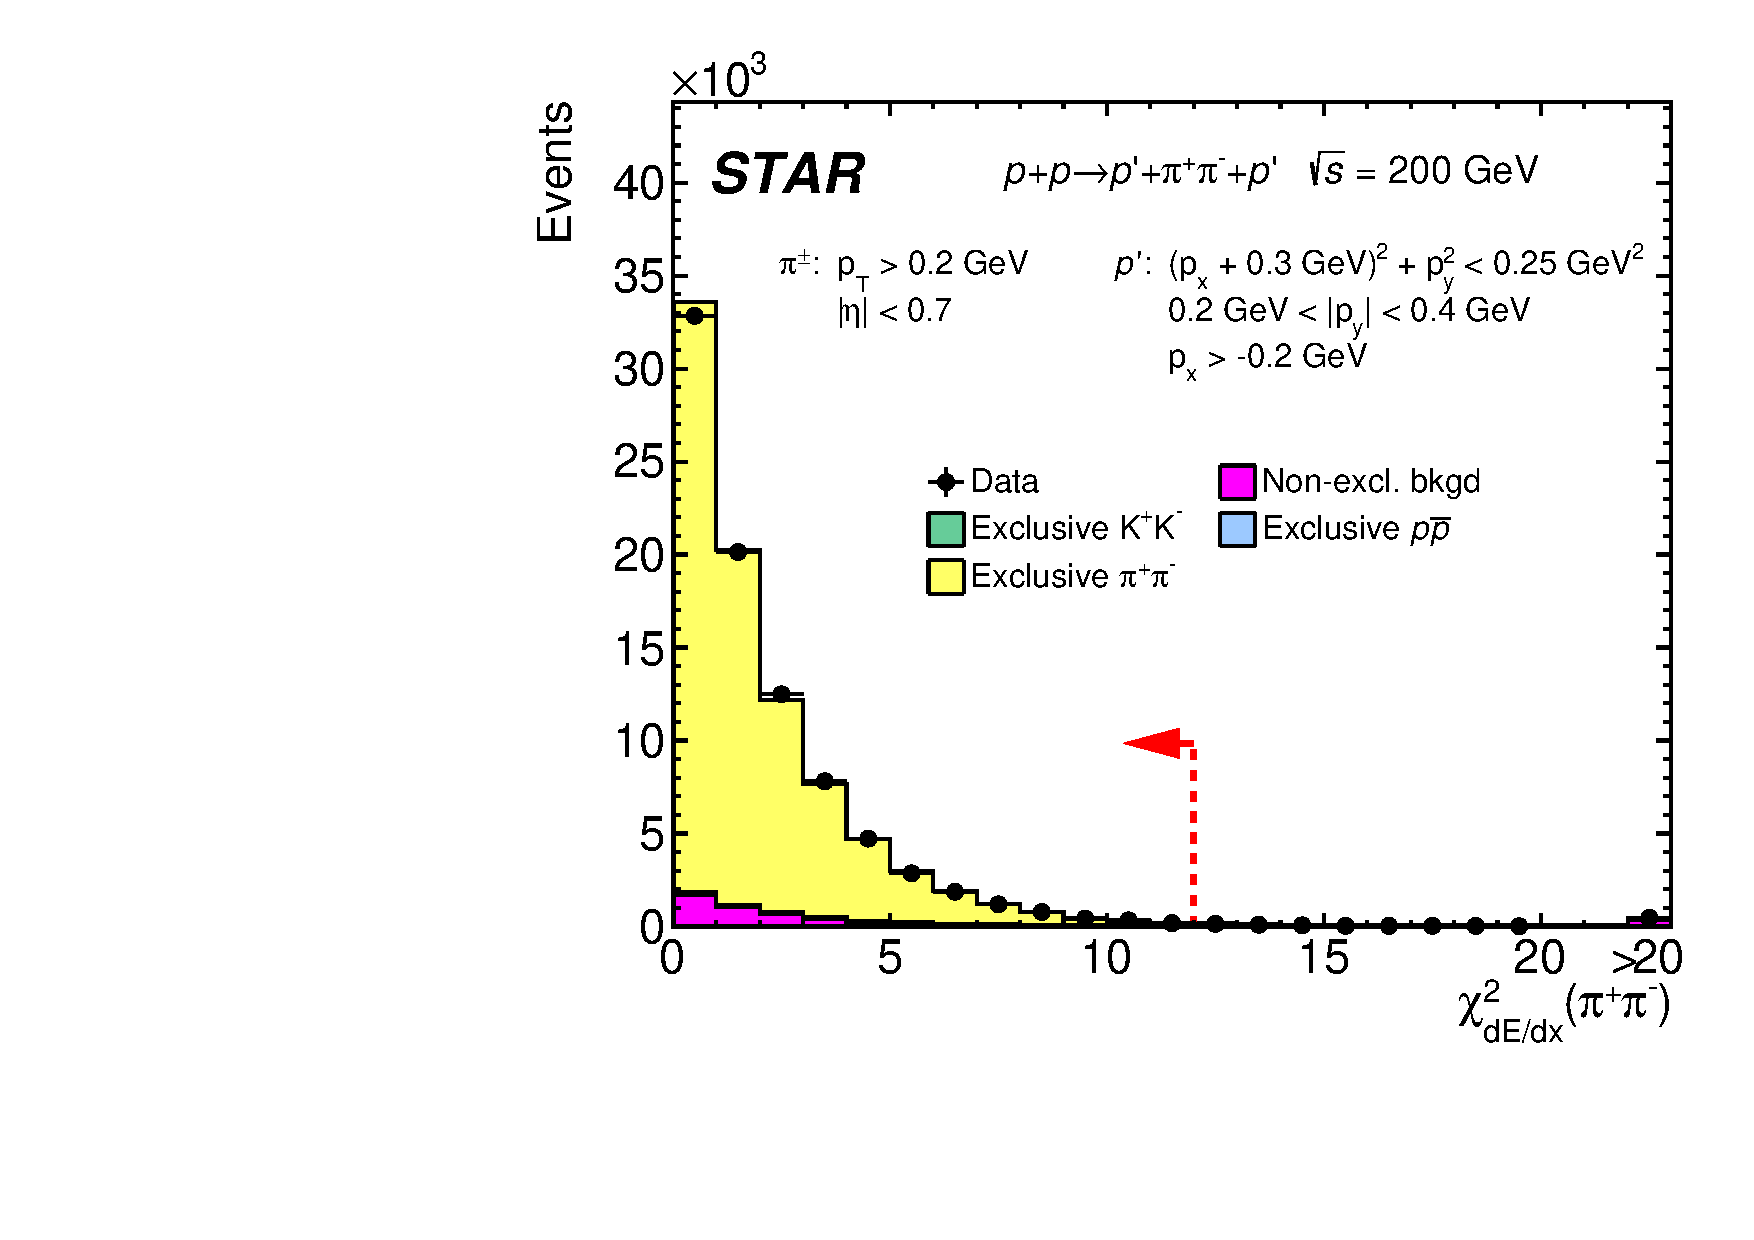
\includegraphics[width=.49\textwidth,page=1]{graphics/eventSelection/pid/Chi2NSigma_pion.pdf}
% \hfill
% 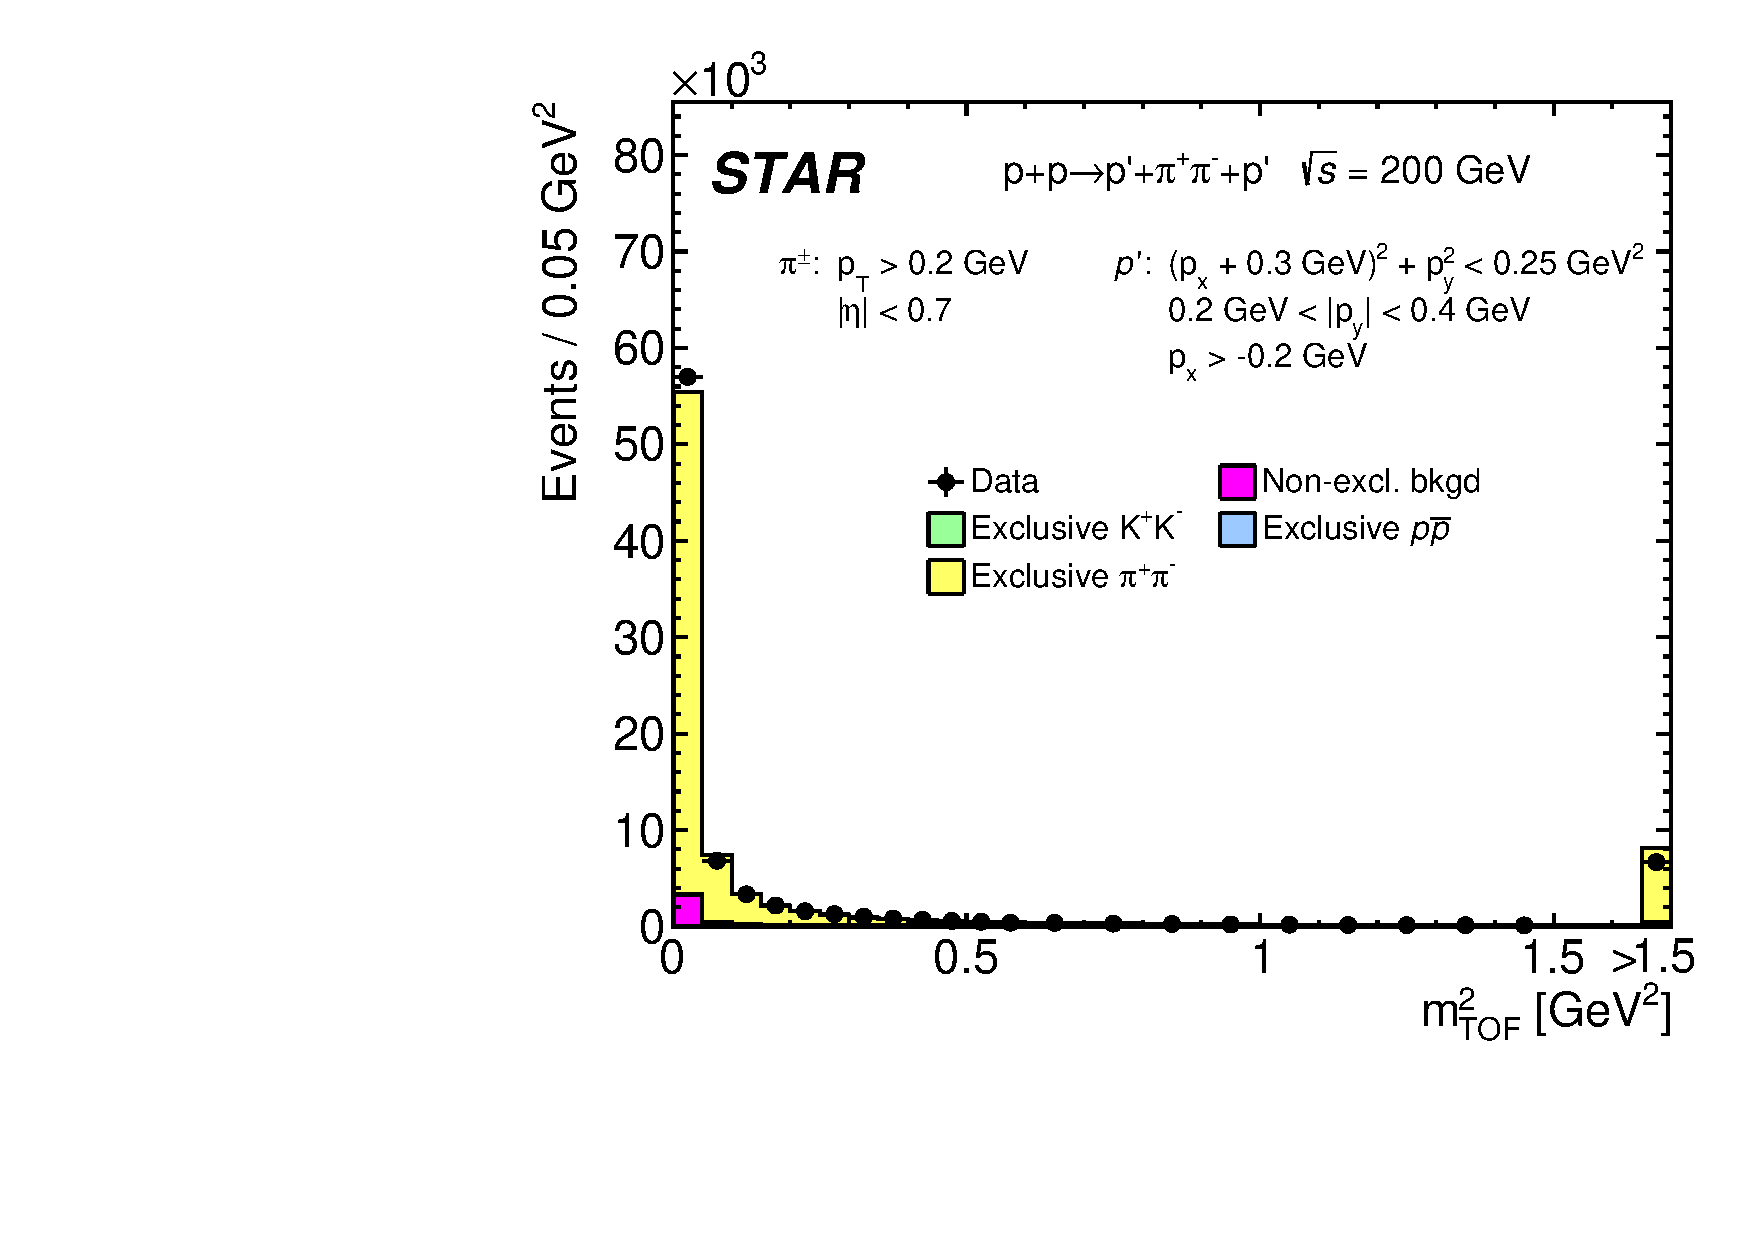
\includegraphics[width=.49\textwidth,page=1]{graphics/eventSelection/pid/SqMassTof_pion.pdf}
% \newline
% \newline
% 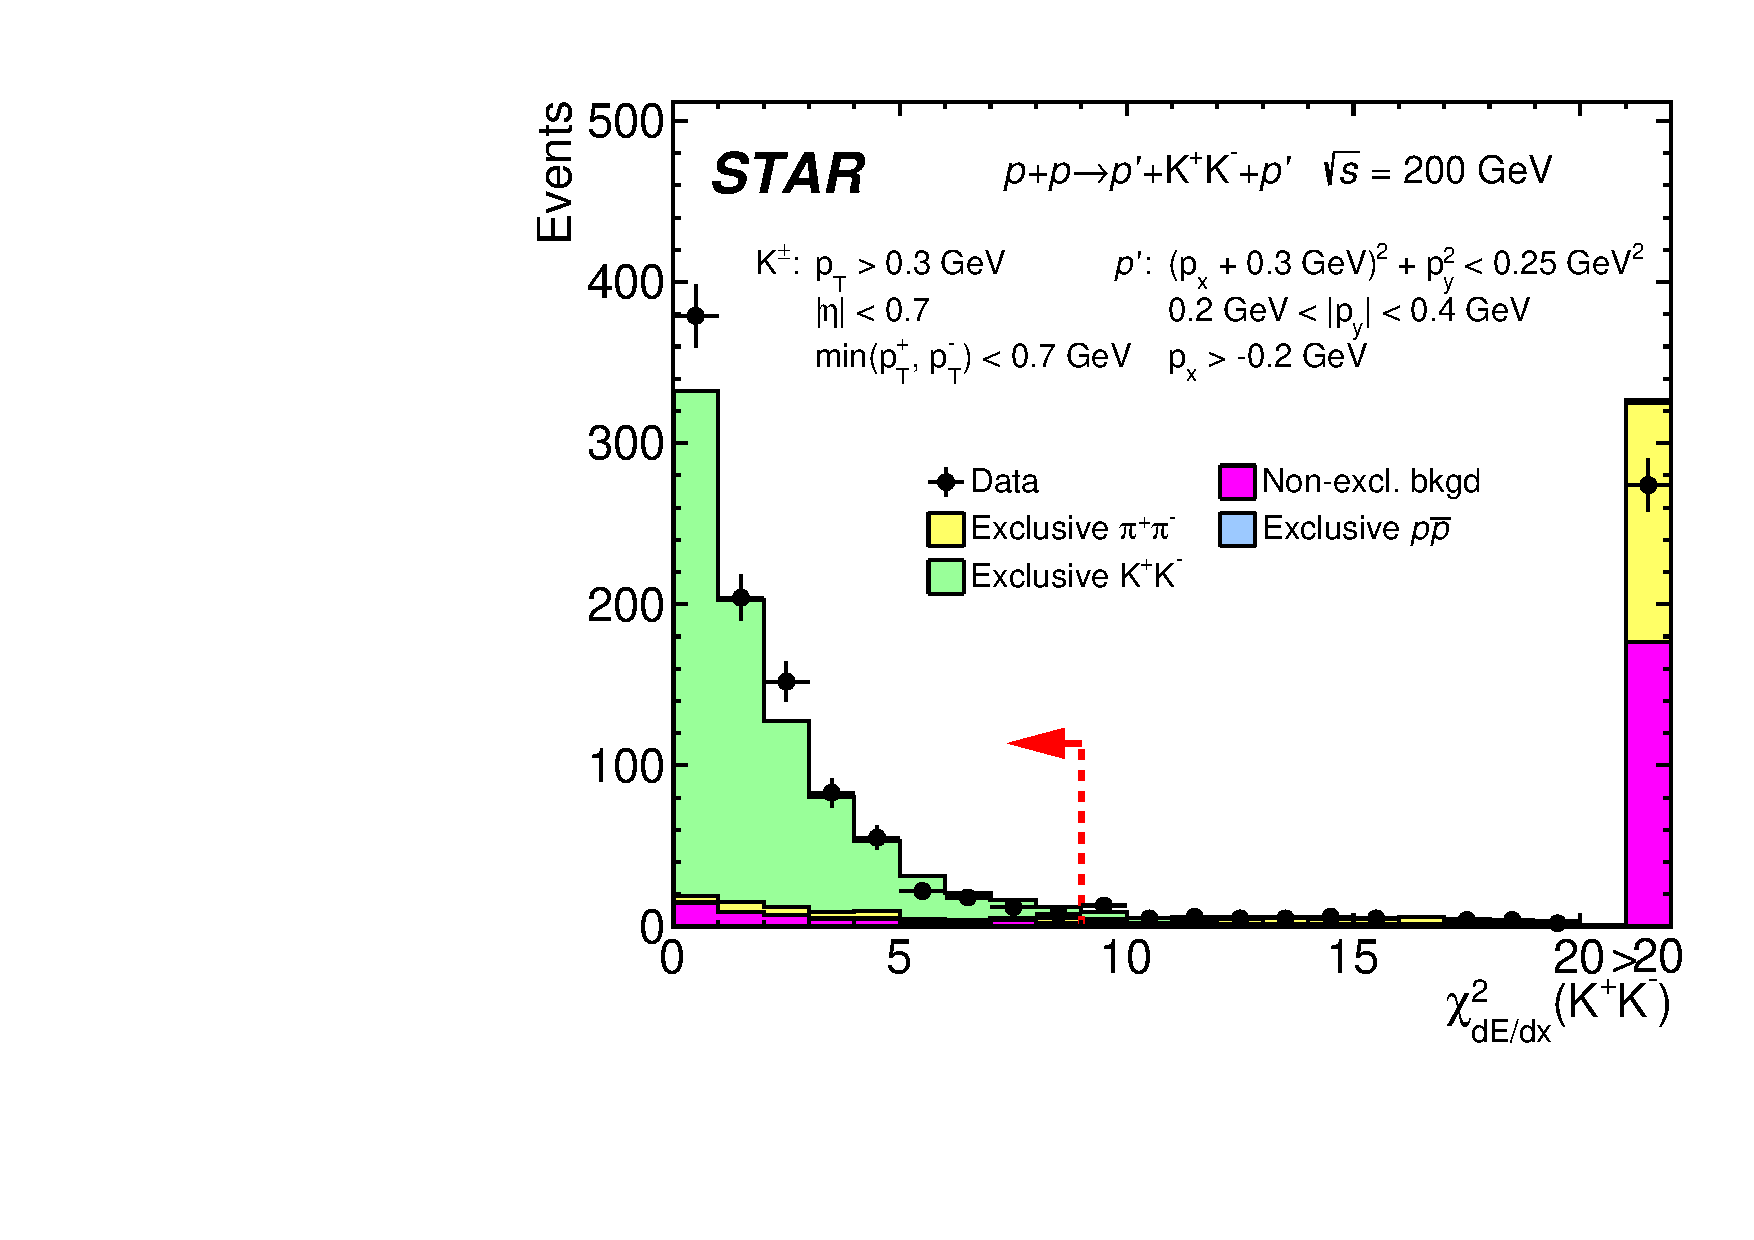
\includegraphics[width=.49\textwidth,page=1]{graphics/eventSelection/pid/Chi2NSigma_kaon.pdf}
% \hfill
% 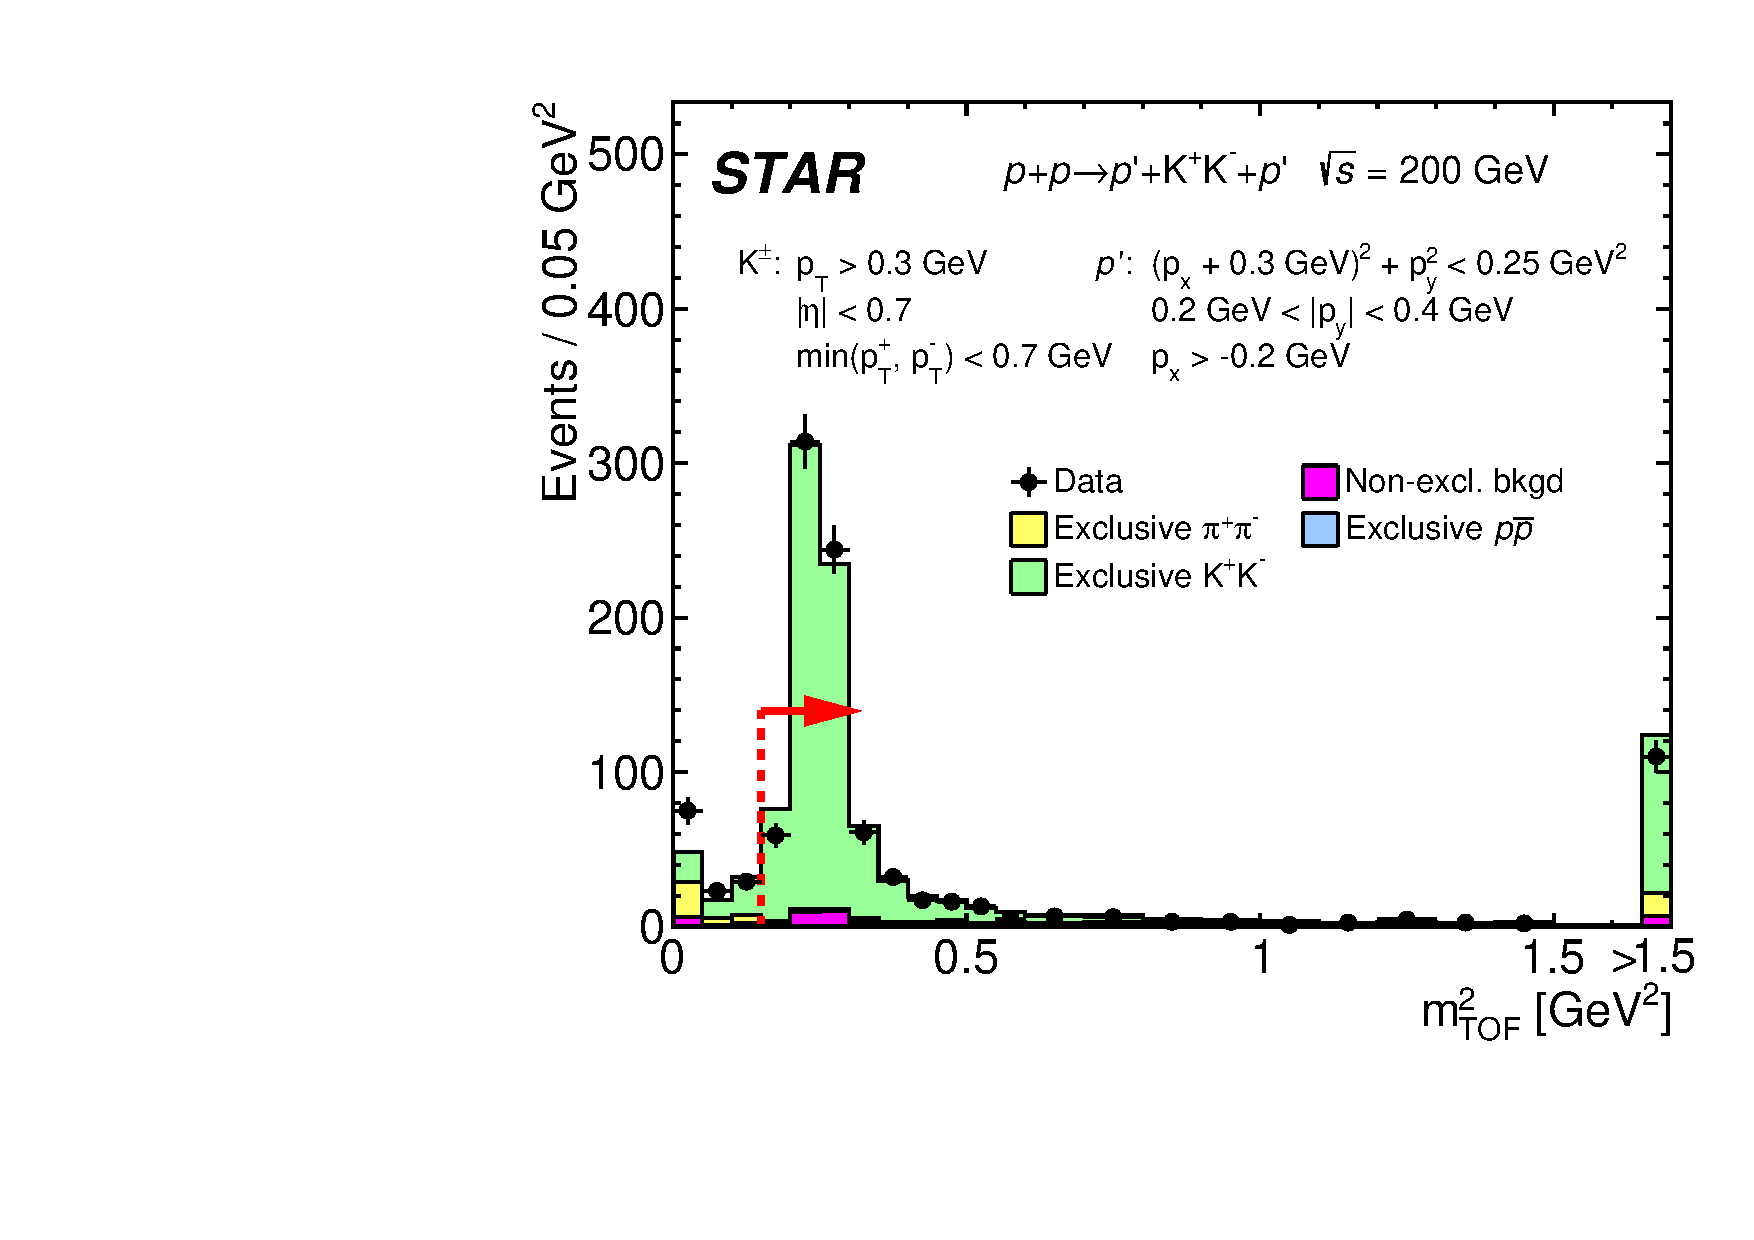
\includegraphics[width=.49\textwidth,page=1]{graphics/eventSelection/pid/SqMassTof_kaon.pdf}
% \newline
% \newline
% 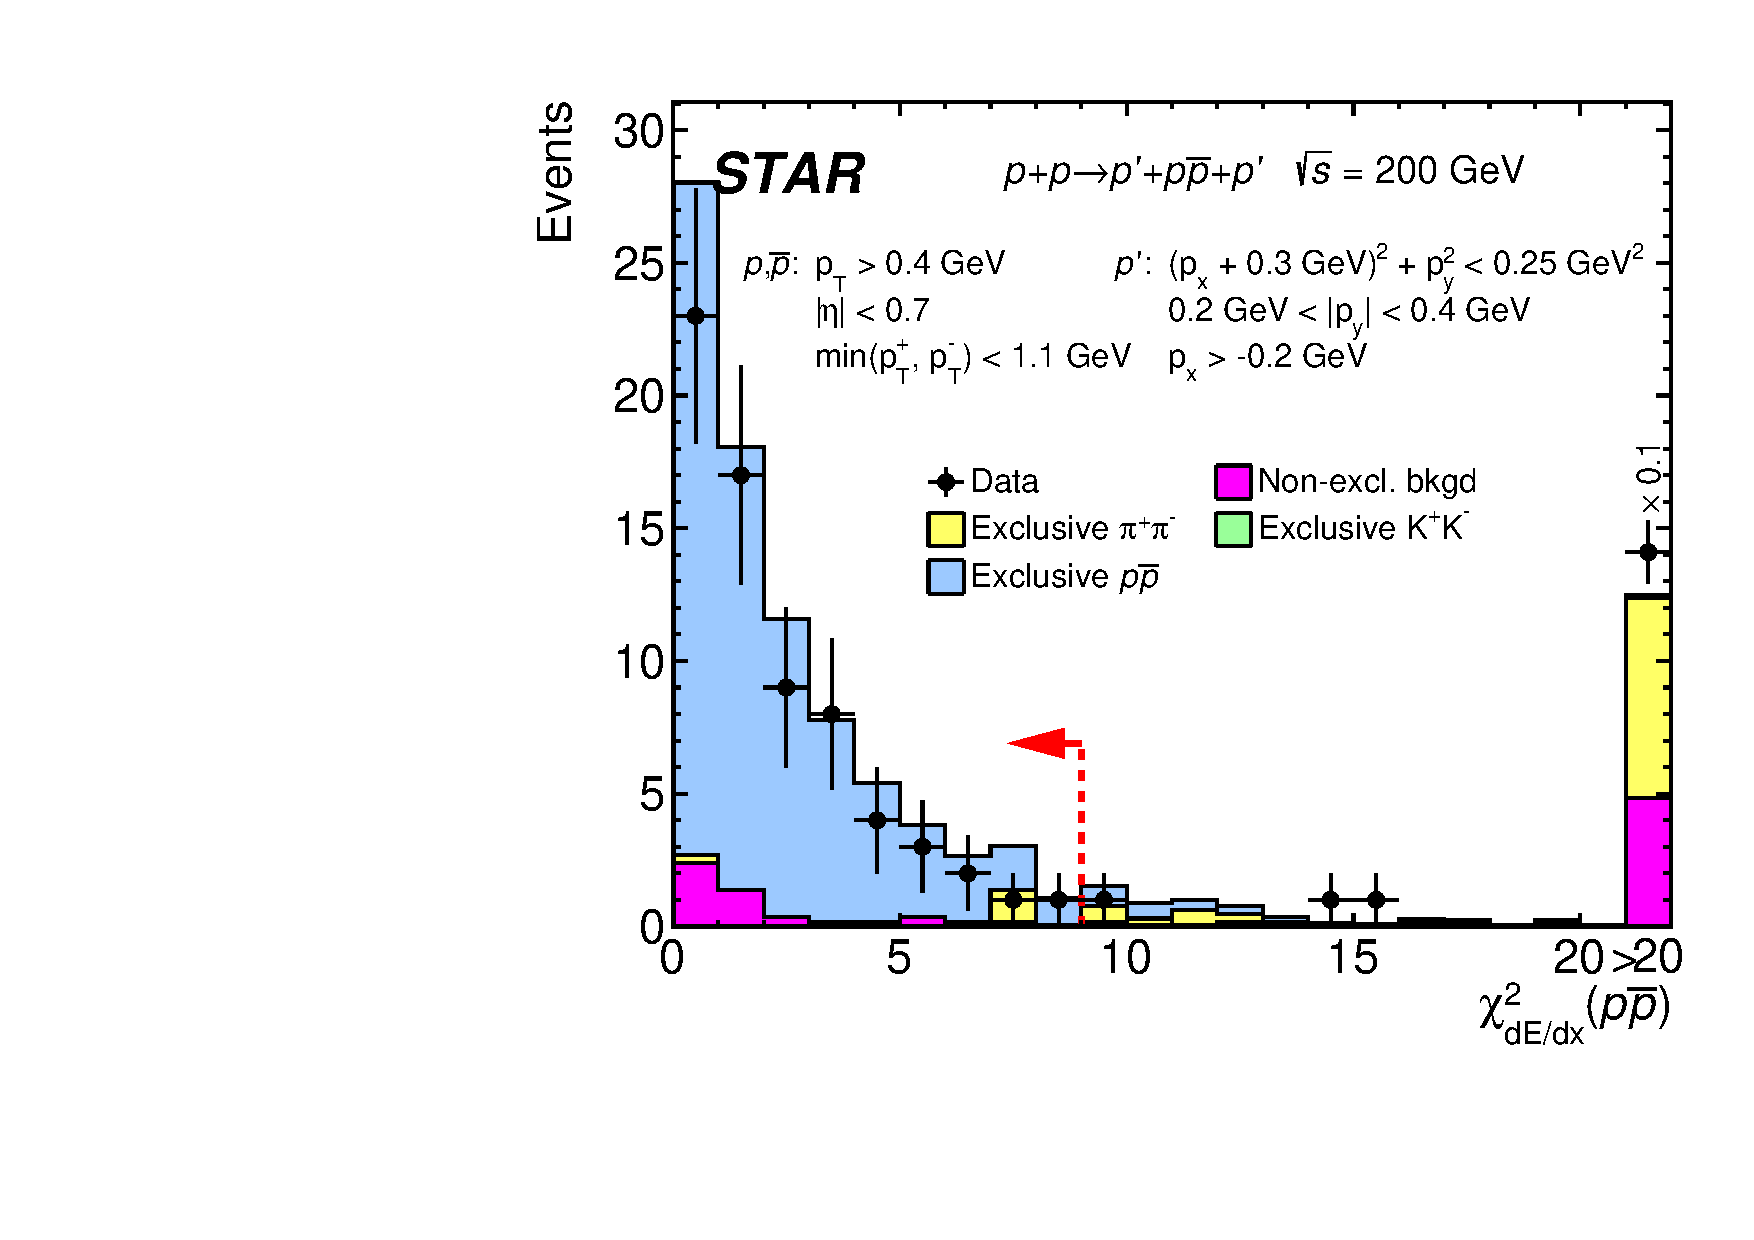
\includegraphics[width=.49\textwidth,page=1]{graphics/eventSelection/pid/Chi2NSigma_proton.pdf}
% \hfill
% 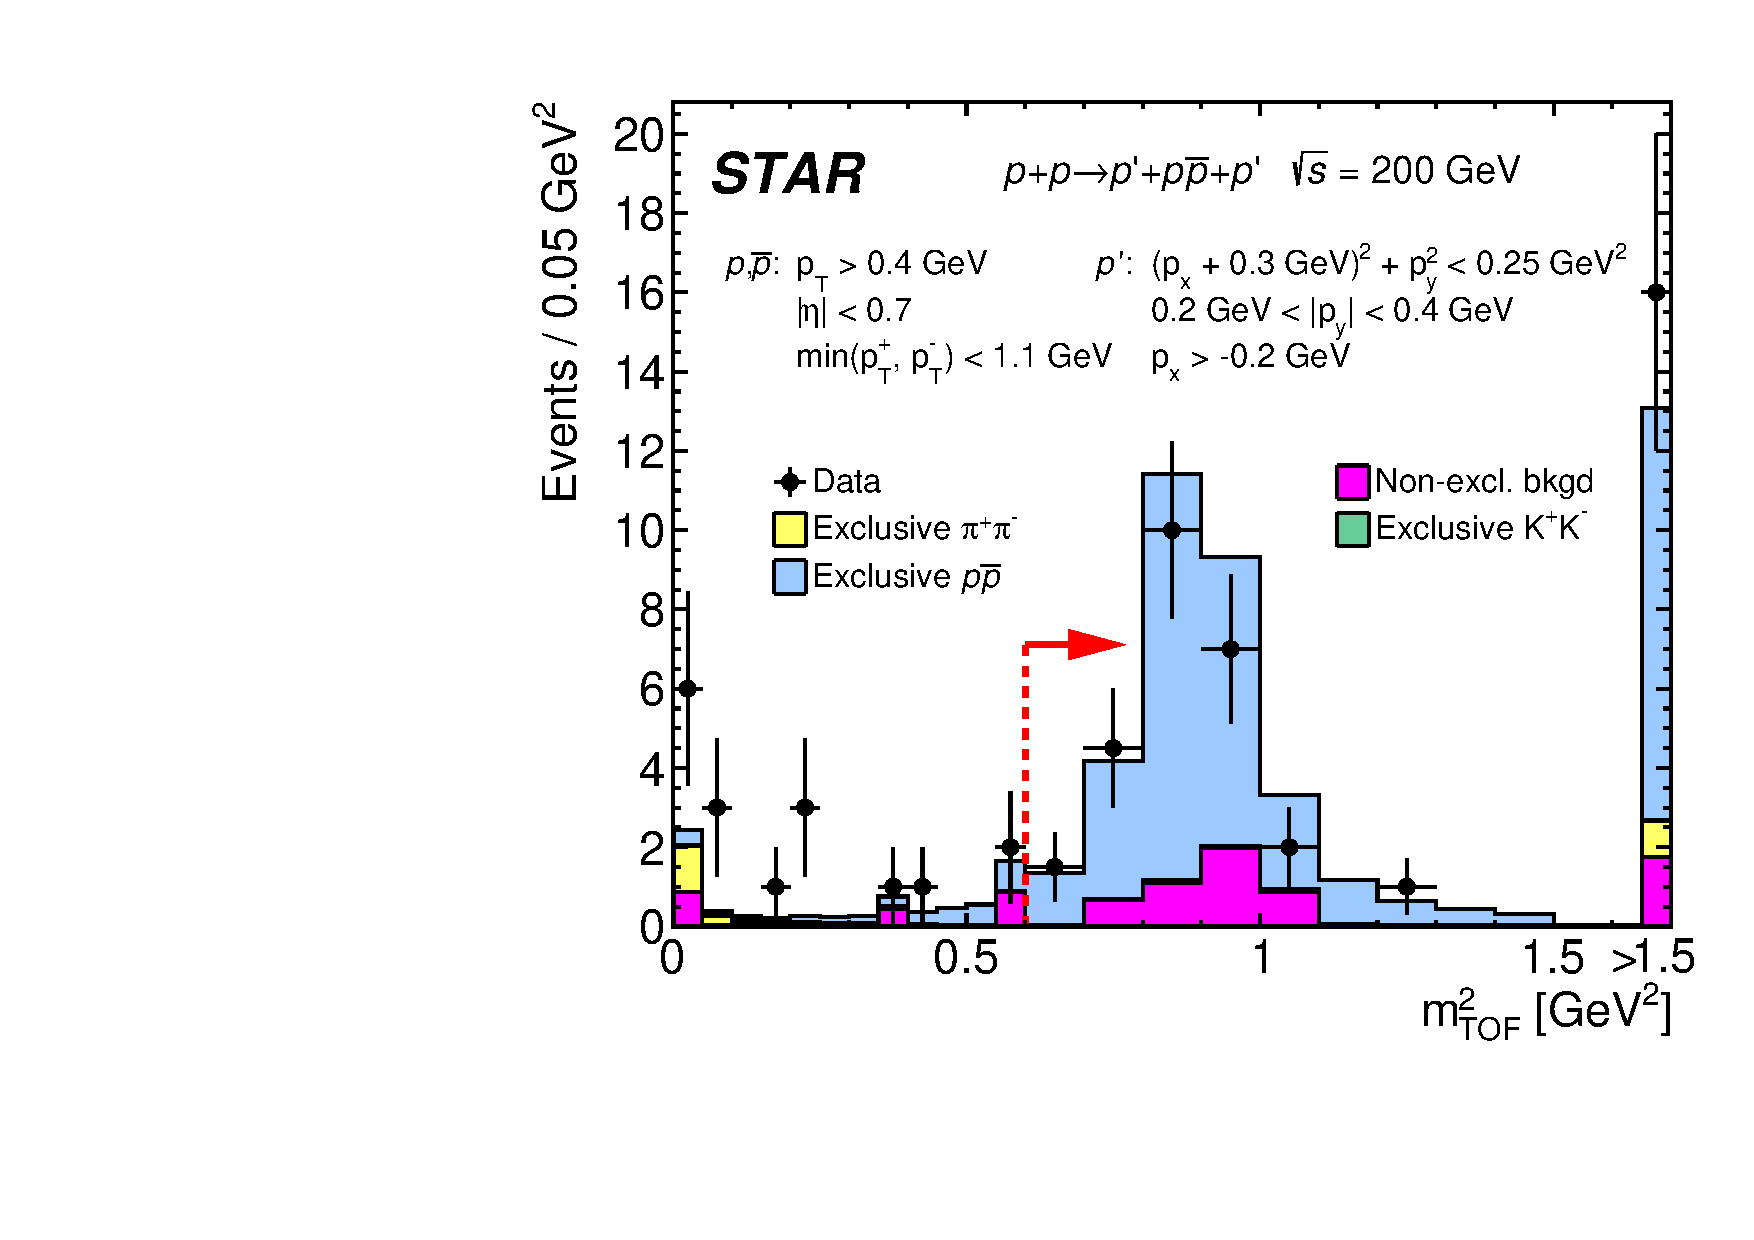
\includegraphics[width=.49\textwidth,page=1]{graphics/eventSelection/pid/SqMassTof_proton.pdf}
% % 
% \caption{Raw distributions of $\chi^{2}_{dE/dx}$ (left column) and $m^{2}_{\text{TOF}}$ (right column) for exclusive $\pi^+\pi^-$ (top row), $K^+K^-$ (middle row) and $p\bar{p}$ (bottom row) candidates after full event selection. Dashed red line and arrow indicate the value of cut imposed on plotted quantity to select exclusive pairs of given particle species.}
% \label{fig:pid_plots} 
% \end{figure}



\begin{figure}[ht!]
  \centering
  \begin{tabular}{@{}p{0.49\linewidth}@{\quad}p{0.49\linewidth}@{}}
    \subfigimg[width=\linewidth,page=1]{~~~~~~~~~~~~~~~~~~~~~~~~~~~~~~~~~~~~~~~~~~~~~~~~~~~~~~~~~~~~~~a)}{graphics/eventSelection/pid/Chi2NSigma_pion.pdf} &
    \subfigimg[width=\linewidth,page=1]{~~~~~~~~~~~~~~~~~~~~~~~~~~~~~~~~~~~~~~~~~~~~~~~~~~~~~~~~~~~~~~c)}{graphics/eventSelection/pid/SqMassTof_pion.pdf} \\
    \subfigimg[width=\linewidth,page=1]{~~~~~~~~~~~~~~~~~~~~~~~~~~~~~~~~~~~~~~~~~~~~~~~~~~~~~~~~~~~~~~d)}{graphics/eventSelection/pid/Chi2NSigma_kaon.pdf} &
    \subfigimg[width=\linewidth,page=1]{~~~~~~~~~~~~~~~~~~~~~~~~~~~~~~~~~~~~~~~~~~~~~~~~~~~~~~~~~~~~~~f)}{graphics/eventSelection/pid/SqMassTof_kaon.pdf} \\
    \subfigimg[width=\linewidth,page=1]{~~~~~~~~~~~~~~~~~~~~~~~~~~~~~~~~~~~~~~~~~~~~~~~~~~~~~~~~~~~~~~g)}{graphics/eventSelection/pid/Chi2NSigma_proton.pdf} &
    \subfigimg[width=\linewidth,page=1]{~~~~~~~~~~~~~~~~~~~~~~~~~~~~~~~~~~~~~~~~~~~~~~~~~~~~~~~~~~~~~~i)}{graphics/eventSelection/pid/SqMassTof_proton.pdf}    
  \end{tabular}
  \caption[$\chi^{2}_{dE/dx}$ and $m^{2}_{\text{TOF}}$ for exclusive $\pi^+\pi^-$, $K^+K^-$ and $p\bar{p}$ candidates.]{Raw distributions of $\chi^{2}_{dE/dx}$ (left column) and $m^{2}_{\text{TOF}}$ (right column) for exclusive $\pi^+\pi^-$ (top row), $K^+K^-$ (middle row) and $p\bar{p}$ (bottom row) candidates after full event selection. Dashed red line and arrow indicate the value of cut imposed on plotted quantity to select exclusive pairs of given particle species. Presented distributions were obtained after all the cuts were applied, except the cut on presented quantity in the last step in PID algorithm used to select pairs of given species.}\label{fig:pid_plots}
\end{figure}

%---------------------------------------------------------------------------------------------------------------

\subsection{(\ref{enum:CutMissingPt})~Exclusivity cut (missing \texorpdfstring{$p_{\text{T}}$}{pT} cut)}

The most important cut which is used in this analysis to select events of exclusively produced pairs of particles is the missing transverse momentum, or the total transverse momentum cut. It benefits from detection and reconstruction of the forward proton in RP detectors - a rare capability among high energy physics experiments which STAR provides. The observable $p_{\text{T}}^{\text{miss}}$ used to select exclusive event is defined as
\begin{equation}\label{eq:missingPt}
 p_{\text{T}}^{\text{miss}} = \Big( \vec{p}_{p'}^{\hspace*{2pt}\text{E}} + \vec{p}_{h^{+}} + \vec{p}_{h^{-}} + \vec{p}_{p'}^{\hspace*{2pt}\text{W}} \Big)_{\text{T}} = \sqrt{\Big(p_{x}^{\text{miss}}\Big)^{2} + \Big(p_{y}^{\text{miss}}\Big)^{2}},
\end{equation}
with the other total momentum components defined analogously:\\
\begin{tabulary}{\textwidth}{LL}
\begin{equation}\label{eq:missingPx}
 p_{x}^{\text{miss}} = \Big( \vec{p}_{p'}^{\hspace*{2pt}\text{E}} + \vec{p}_{h^{+}} + \vec{p}_{h^{-}} + \vec{p}_{p'}^{\hspace*{2pt}\text{W}} \Big)_{x},
\end{equation}~~~~~~~~~~~~~~~~~~~~~
&
\begin{equation}\label{eq:missingPy}
 p_{y}^{\text{miss}} = \Big( \vec{p}_{p'}^{\hspace*{2pt}\text{E}} + \vec{p}_{h^{+}} + \vec{p}_{h^{-}} + \vec{p}_{p'}^{\hspace*{2pt}\text{W}} \Big)_{y}.
\end{equation}~~~~~~~~~~~~~~~~~~~~~
\end{tabulary}


Figure~\ref{fig:PxPyCentralTrksVsProtons} visualize the (anti-)correlation between the momentum components of the forward system (sum of forward protons momenta) and the central system (sum of central tracks momenta). The enhanced band at anti-diagonal restricted by dashed lines contains events balanced in momentum, a signature of exclusivity. Events outside this band are the non exclusive backgrounds, in most cases Central Diffraction events with some particles undected (due to detector inefficiency or produced outside acceptance). Slight horizontal enhancement in all distributions around $[\vec{p}^{\hspace*{2pt}\text{W}}_{p'}+\vec{p}^{\hspace*{2pt}\text{E}}_{p'}]_{x} = [\vec{p}^{\hspace*{2pt}\text{W}}_{p'}+\vec{p}^{\hspace*{2pt}\text{E}}_{p'}]_{x} =0$ is a signature of the elastic proton-proton scattering background with some non-elastic pile-up interaction which mimics the CEP event. All these backgrounds are reasonably low after the exclusivity cut, as described in Sec.~\ref{sec:nonExclBkgd}.

The momentum balance is shown one-dimensionally in Fig.~\ref{fig:MissingPxPy}, with the sum of $x$- and $y$-components of momentum shown repectively in the left and right column for each analyzed particle species. The sum of signal and background (both assumed to be described a Gaussian) was fitted to $p_{x}^{\text{miss}}$ and $p_{y}^{\text{miss}}$ distributions. Results of the fit are given in each subfigure. One can notice that the widths of Gaussian functions representing the exclusive signal are consistent among species and amount $\sigma_{p_{x}^{\text{miss}}}=27.4$~MeV for the $x$-component of total momentum, and $\sigma_{p_{y}^{\text{miss}}}=28.1$~MeV for the $y$-component of total momentum, taking the values of the lowest statistical uncertainty - for $\pi^{+}\pi^{-}$. These values are measures of the total momentum resolution respectivelty for $p_{x}^{\text{miss}}$ and $p_{y}^{\text{miss}}$. Having these number it is possible to form an elliptical on the missing momentum:

\begin{equation}\label{eq:ptMissEllipse}%
\left(\frac{p_{x}^{\text{miss}}}{\sigma_{p_{x}^{\text{miss}}}}\right)^{2} + \left(\frac{p_{y}^{\text{miss}}}{\sigma_{p_{y}^{\text{miss}}}}\right)^{2} < n_{\text{cut}}^{2}
\end{equation}
%
where $n_{\text{cut}}$ is the parameter denoting radius of limiting ellipsis in units of standard deviations of distributions of total momentum components (resolutions). Since these resolutions are nearly identical ($\sigma_{p_{x}^{\text{miss}}} = \sigma_{p_{y}^{\text{miss}}} = \sigma_{p_{x,y}^{\text{miss}}}$) such cut can be reduced (multiplying Ineq.~\ref{eq:ptMissEllipse} by $\sigma_{p_{x,y}^{\text{miss}}}^{2}$) to one-dimensional cut on a single quantity:

\begin{equation}%
\left(p_{x}^{\text{miss}}\right)^{2} + \left(p_{y}^{\text{miss}}\right)^{2} < \Big(n_{\text{cut}}\cdot\sigma_{p_{x,y}^{\text{miss}}}\Big)^{2}~~~~~~~\xrightarrow[~]{\sqrt{~}}~~~~~~~p_{\text{T}}^{\text{miss}} < n_{\text{cut}}\cdot\sigma_{p_{x,y}^{\text{miss}}}~~~~
\end{equation}%
%
In current analysis the $n_{\text{cut}}$ was set to 2.5, which translates to threshold value $2.5\times 30~\text{MeV} = 75$~MeV.



\begin{figure}[ht!]\vspace*{-20pt}
  \centering
  \begin{tabular}{@{}p{0.47\linewidth}@{\quad\quad}p{0.47\linewidth}@{}}
    \subfigimg[width=\linewidth,page=1]{~~~~~~~~~~~~~~~~a)}{graphics/eventSelection/exclusivity/PxCentralTrksVsProtons_pion.pdf} &
    \subfigimg[width=\linewidth,page=1]{~~~~~~~~~~~~~~~~~~~~~~c)}{graphics/eventSelection/exclusivity/PyCentralTrksVsProtons_pion.pdf} \\[-10pt]
    \subfigimg[width=\linewidth,page=1]{~~~~~~~~~~~~~~~~d)}{graphics/eventSelection/exclusivity/PxCentralTrksVsProtons_kaon.pdf} &
    \subfigimg[width=\linewidth,page=1]{~~~~~~~~~~~~~~~~~~~~~~f)}{graphics/eventSelection/exclusivity/PyCentralTrksVsProtons_kaon.pdf} \\[-10pt]
    \subfigimg[width=\linewidth,page=1]{~~~~~~~~~~~~~~~~g)}{graphics/eventSelection/exclusivity/PxCentralTrksVsProtons_proton.pdf} &
    \subfigimg[width=\linewidth,page=1]{~~~~~~~~~~~~~~~~~~~~~~i)}{graphics/eventSelection/exclusivity/PyCentralTrksVsProtons_proton.pdf}    
  \end{tabular}\vspace*{-5pt}
    \caption[Two-dimensional distributions of sum of forward protons momenta and sum of central tracks momenta for exclusive $\pi^+\pi^-$ (top row), $K^+K^-$ (middle row) and $p\bar{p}$ (bottom row) event candidates.]{Two-dimensional distributions of sum of forward protons momenta ($x$-axis) and sum of central tracks momenta ($y$-axis) for exclusive $\pi^+\pi^-$ (top row), $K^+K^-$ (middle row) and $p\bar{p}$ (bottom row) event candidates after full event selection, except the exclusivity cut~\ref{enum:CutMissingPt}. Left and right column shows correlation of respectivelty $x$- and $y$-component of tracks' momenta. Anti-diagonal representing perfect momentum balance of the central and forward system is limited with dashed lines extending by $\pm2.5\sigma$  ($\sigma\approx 30$~MeV) around the anti-diagonal. Three distinct horizontal regions in plots on the right hand side correspond to different forward proton configurations: elastic-like (protons in branches EU\&WD or ED\&WU, $\left|[\vec{p}^{\hspace*{2pt}\text{W}}_{p'}+\vec{p}^{\hspace*{2pt}\text{E}}_{p'}]_{y}\right| < 0.2$~GeV) and anti-elastic configuration (protons in branches ED\&WD or EU\&WU, $\left|[\vec{p}^{\hspace*{2pt}\text{W}}_{p'}+\vec{p}^{\hspace*{2pt}\text{E}}_{p'}]_{y}\right| > 0.4$~GeV).}\label{fig:PxPyCentralTrksVsProtons}
\end{figure}




\begin{figure}[ht!]
  \centering
  \begin{tabular}{@{}p{0.49\linewidth}@{\quad\quad}p{0.49\linewidth}@{}}
    \subfigimg[width=\linewidth,page=1]{~~~~~~~~~~~~~~~~~~~~~~~~~~~~~~~~~~~~~~~~~~~~~~~~~~~~~~~~~~~~~a)}{graphics/eventSelection/exclusivity/MissingPx_pion.pdf} &
    \subfigimg[width=\linewidth,page=1]{~~~~~~~~~~~~~~~~~~~~~~~~~~~~~~~~~~~~~~~~~~~~~~~~~~~~~~~~~~~~~b)}{graphics/eventSelection/exclusivity/MissingPy_pion.pdf} \\
    \subfigimg[width=\linewidth,page=1]{~~~~~~~~~~~~~~~~~~~~~~~~~~~~~~~~~~~~~~~~~~~~~~~~~~~~~~~~~~~~~c)}{graphics/eventSelection/exclusivity/MissingPx_kaon.pdf} &
    \subfigimg[width=\linewidth,page=1]{~~~~~~~~~~~~~~~~~~~~~~~~~~~~~~~~~~~~~~~~~~~~~~~~~~~~~~~~~~~~~d)}{graphics/eventSelection/exclusivity/MissingPy_kaon.pdf} \\
    \subfigimg[width=\linewidth,page=1]{~~~~~~~~~~~~~~~~~~~~~~~~~~~~~~~~~~~~~~~~~~~~~~~~~~~~~~~~~~~~~e)}{graphics/eventSelection/exclusivity/MissingPx_proton.pdf} &
    \subfigimg[width=\linewidth,page=1]{~~~~~~~~~~~~~~~~~~~~~~~~~~~~~~~~~~~~~~~~~~~~~~~~~~~~~~~~~~~~~f)}{graphics/eventSelection/exclusivity/MissingPy_proton.pdf}    
  \end{tabular}\vspace*{-5pt}
    \caption[Raw distributions of $p_{x}^{\text{miss}}$ and $p_{y}^{\text{miss}}$ for exclusive $\pi^+\pi^-$, $K^+K^-$ and $p\bar{p}$candidates.]{%
    Raw distributions of $p_{x}^{\text{miss}}$ (left column) and $p_{y}^{\text{miss}}$ (right column) for exclusive $\pi^+\pi^-$ (top row), $K^+K^-$ (middle row) and $p\bar{p}$ (bottom row) candidates after full event selection, except exclusivity cut~\ref{enum:CutMissingPt}. Solid red line represents the fit of sum of two Gaussian functions representing the exclusive event signal (orange) and non-exclusive background (violet). Parameters of the total momentum resolution for signal events obtained from the fit (given in the plots) roughly agree between all species.
    }\label{fig:MissingPxPy}
\end{figure}




%---------------------------
\begin{figure}[ht!]
% \begin{wrapfigure}{l}{0.475\textwidth}%[ht!]
\centering%
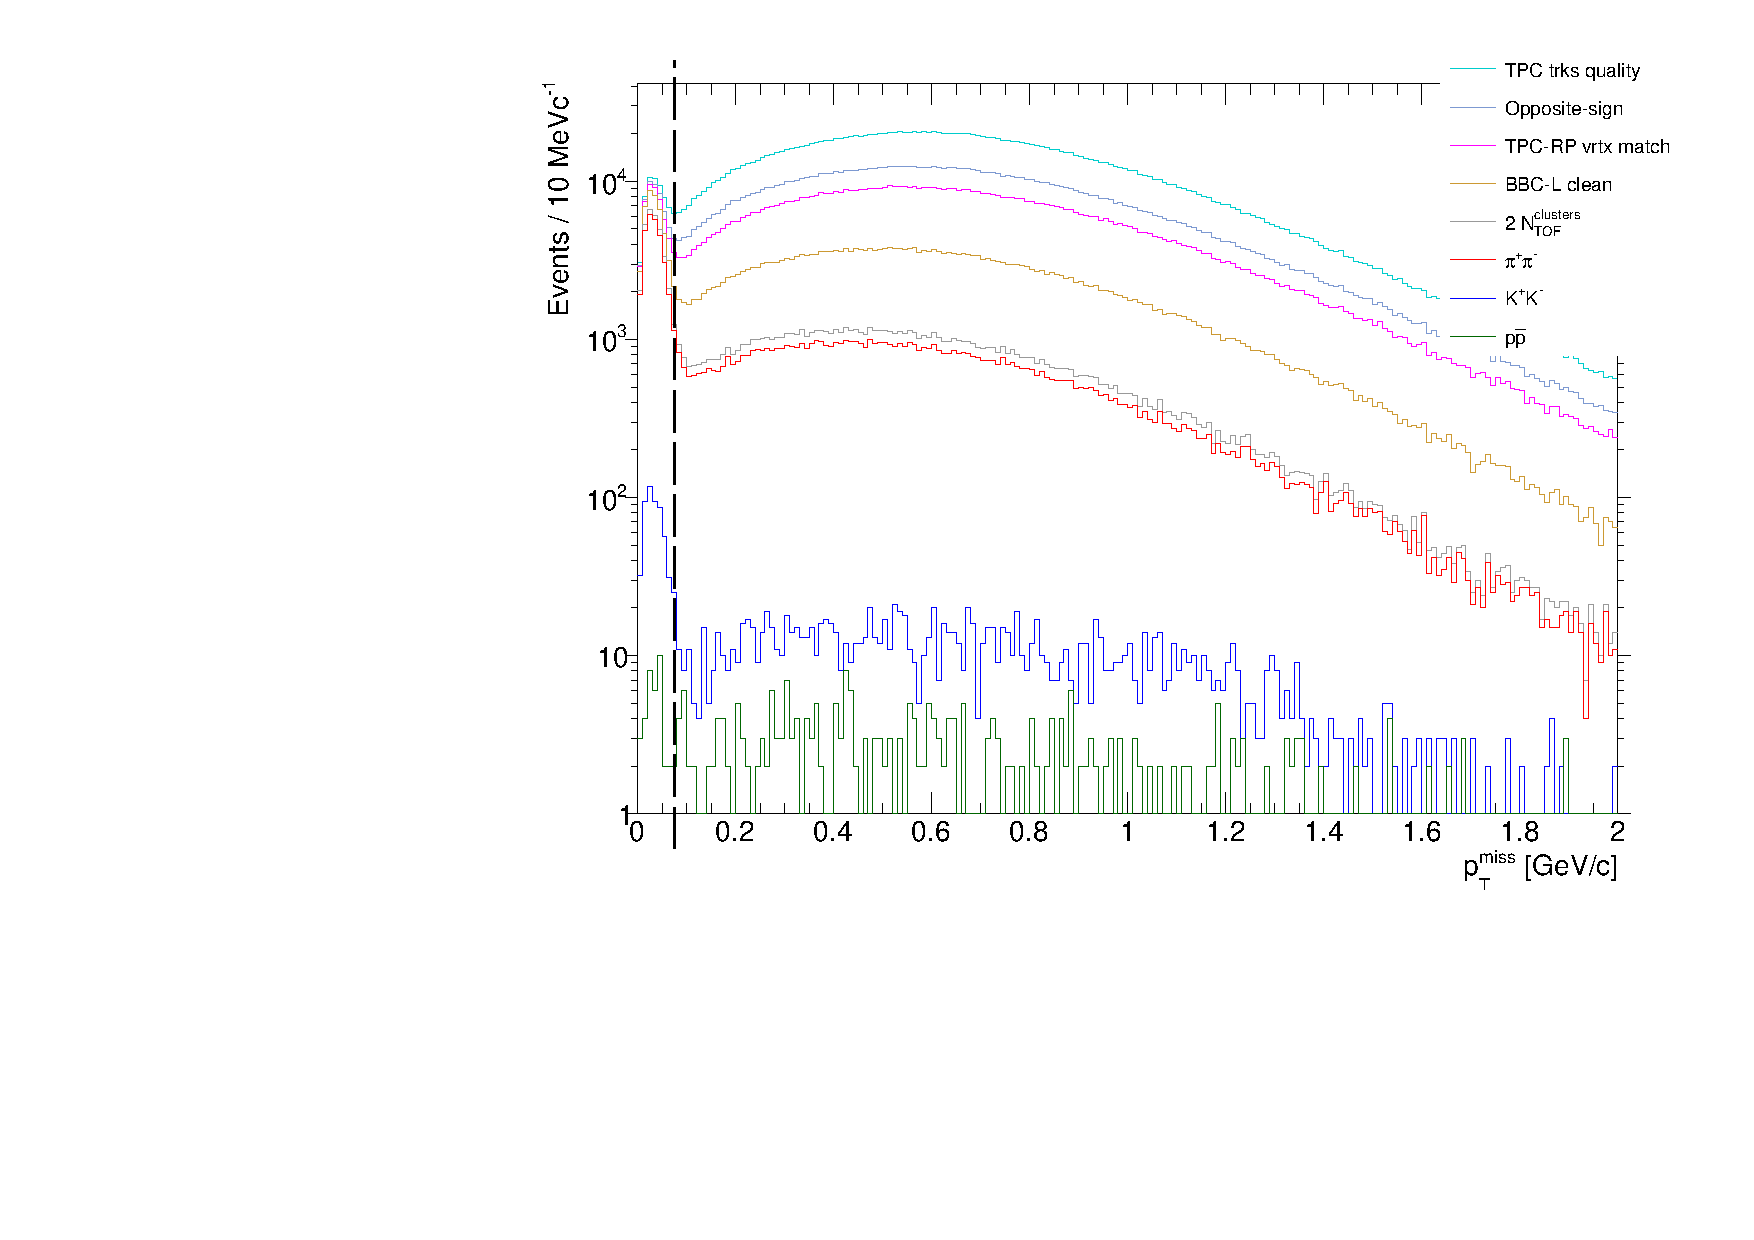
\includegraphics[width=0.633\linewidth,page=1]{graphics/eventSelection/MissingPt.pdf}%
% % 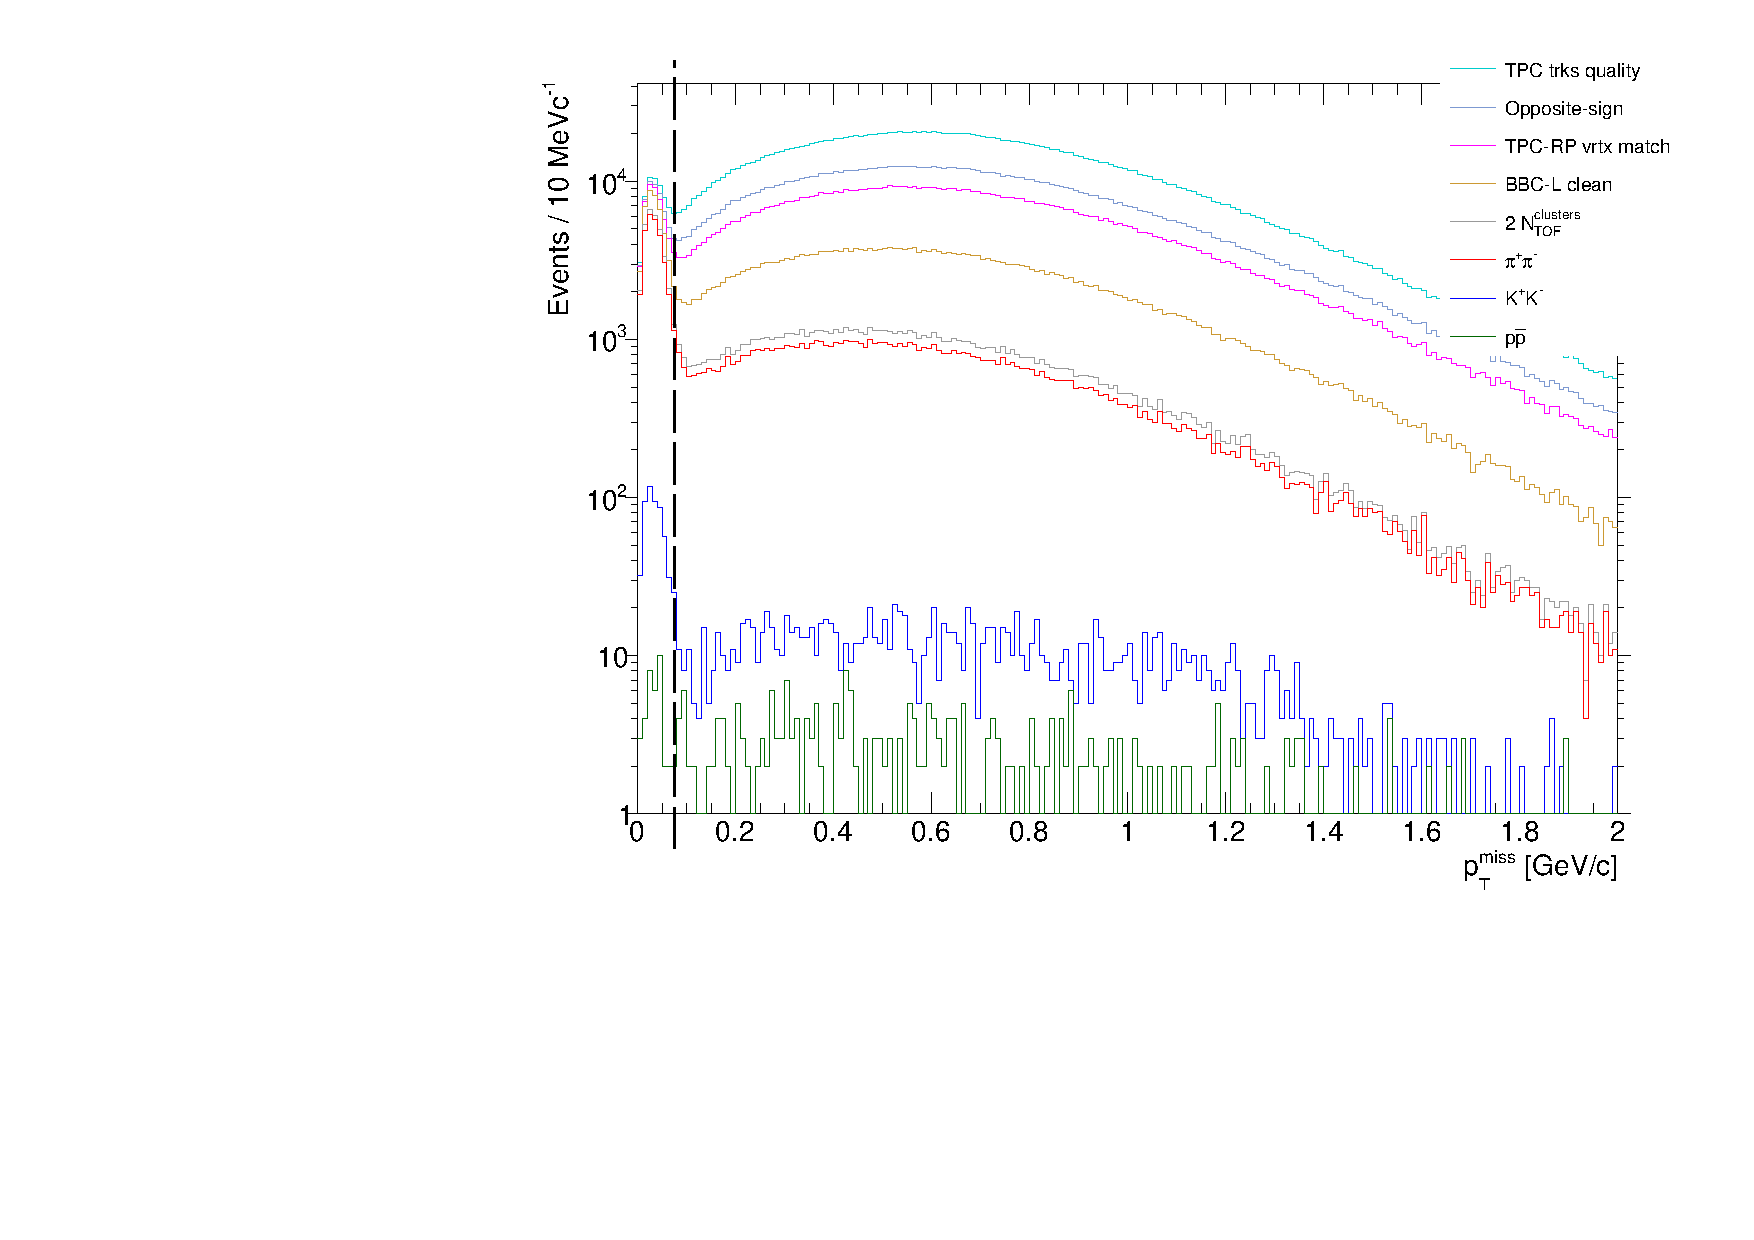
\includegraphics[width=\linewidth,page=1]{graphics/eventSelection/MissingPt.pdf}%
\caption{MissingPt.}\label{fig:MissingPt}%
\end{figure}
% \end{wrapfigure}
%---------------------------

 





% 
% \section{Working point for cuts~\ref{enum:CutBbcLarge}, \ref{enum:CutTofClusters} and \ref{enum:CutMissingPt}}
% 
% \begin{tabulary}{\textwidth}{LLL}
% \begin{equation}\label{eq:significance}\hspace*{-10pt}
% 	\text{Significance} = \frac{N_{\text{signal}}^{\text{cut}}}{\sqrt{N_{\text{signal}}^{\text{cut}} + N_{\text{bkgd}}^{\text{cut}}}},
% \end{equation}~~~~~~~~~~~~~~~~~&
% \begin{equation}\label{eq:efficiency}\hspace*{-10pt}
% 	\text{Efficiency} = \frac{N_{\text{signal}}^{\text{cut}}}{N_{\text{signal}}^{\text{no~cut}}},
% \end{equation}~~~~~~~~~~~~~~&
% \begin{equation}\label{eq:purity}\hspace*{-9pt}
% 	\text{Purity} = \frac{N_{\text{signal}}^{\text{cut}}}{N_{\text{signal}}^{\text{cut}}+N_{\text{bkgd}}^{\text{cut}}},
% \end{equation}~~~~~~~~~~~~~~~
% \end{tabulary}
% 
% 
% %---------------------------
% \begin{figure}[hb]
% \centering
% \parbox{0.4725\textwidth}{
%   \centering
%   \begin{subfigure}[b]{\linewidth}
%                 \subcaptionbox{\label{fig:SignificanceVsEff}}{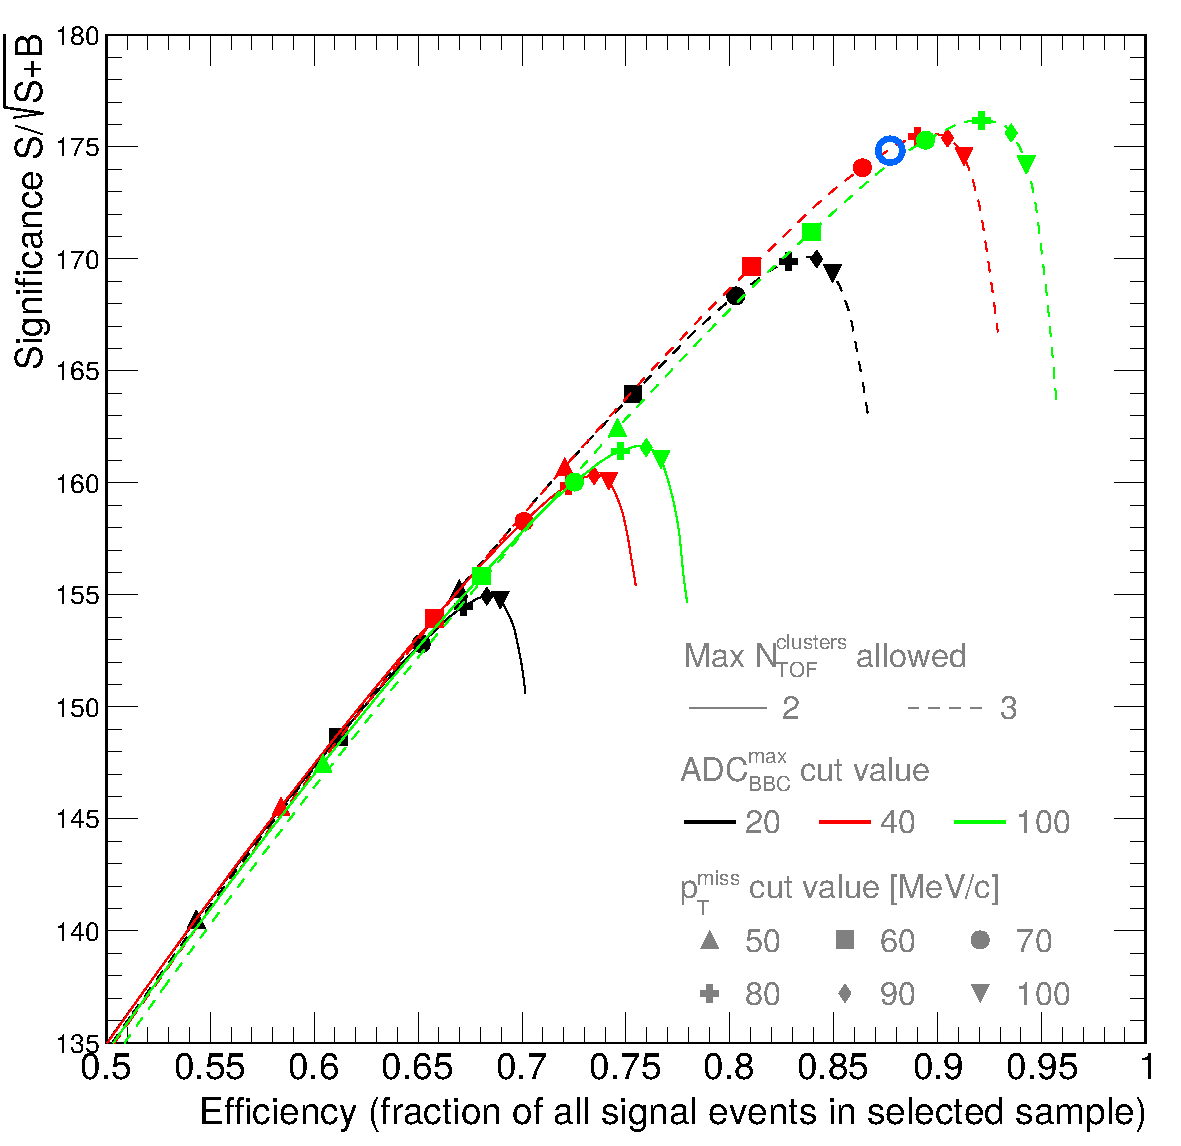
\includegraphics[width=\linewidth]{graphics/eventSelection/SignificanceVsEfficiency_pTmiss.pdf}}
%   \end{subfigure}\\
%   \begin{subfigure}[b]{\linewidth}\addtocounter{subfigure}{1}
%                 \subcaptionbox{\label{fig:EffVsBkgdFrac}}{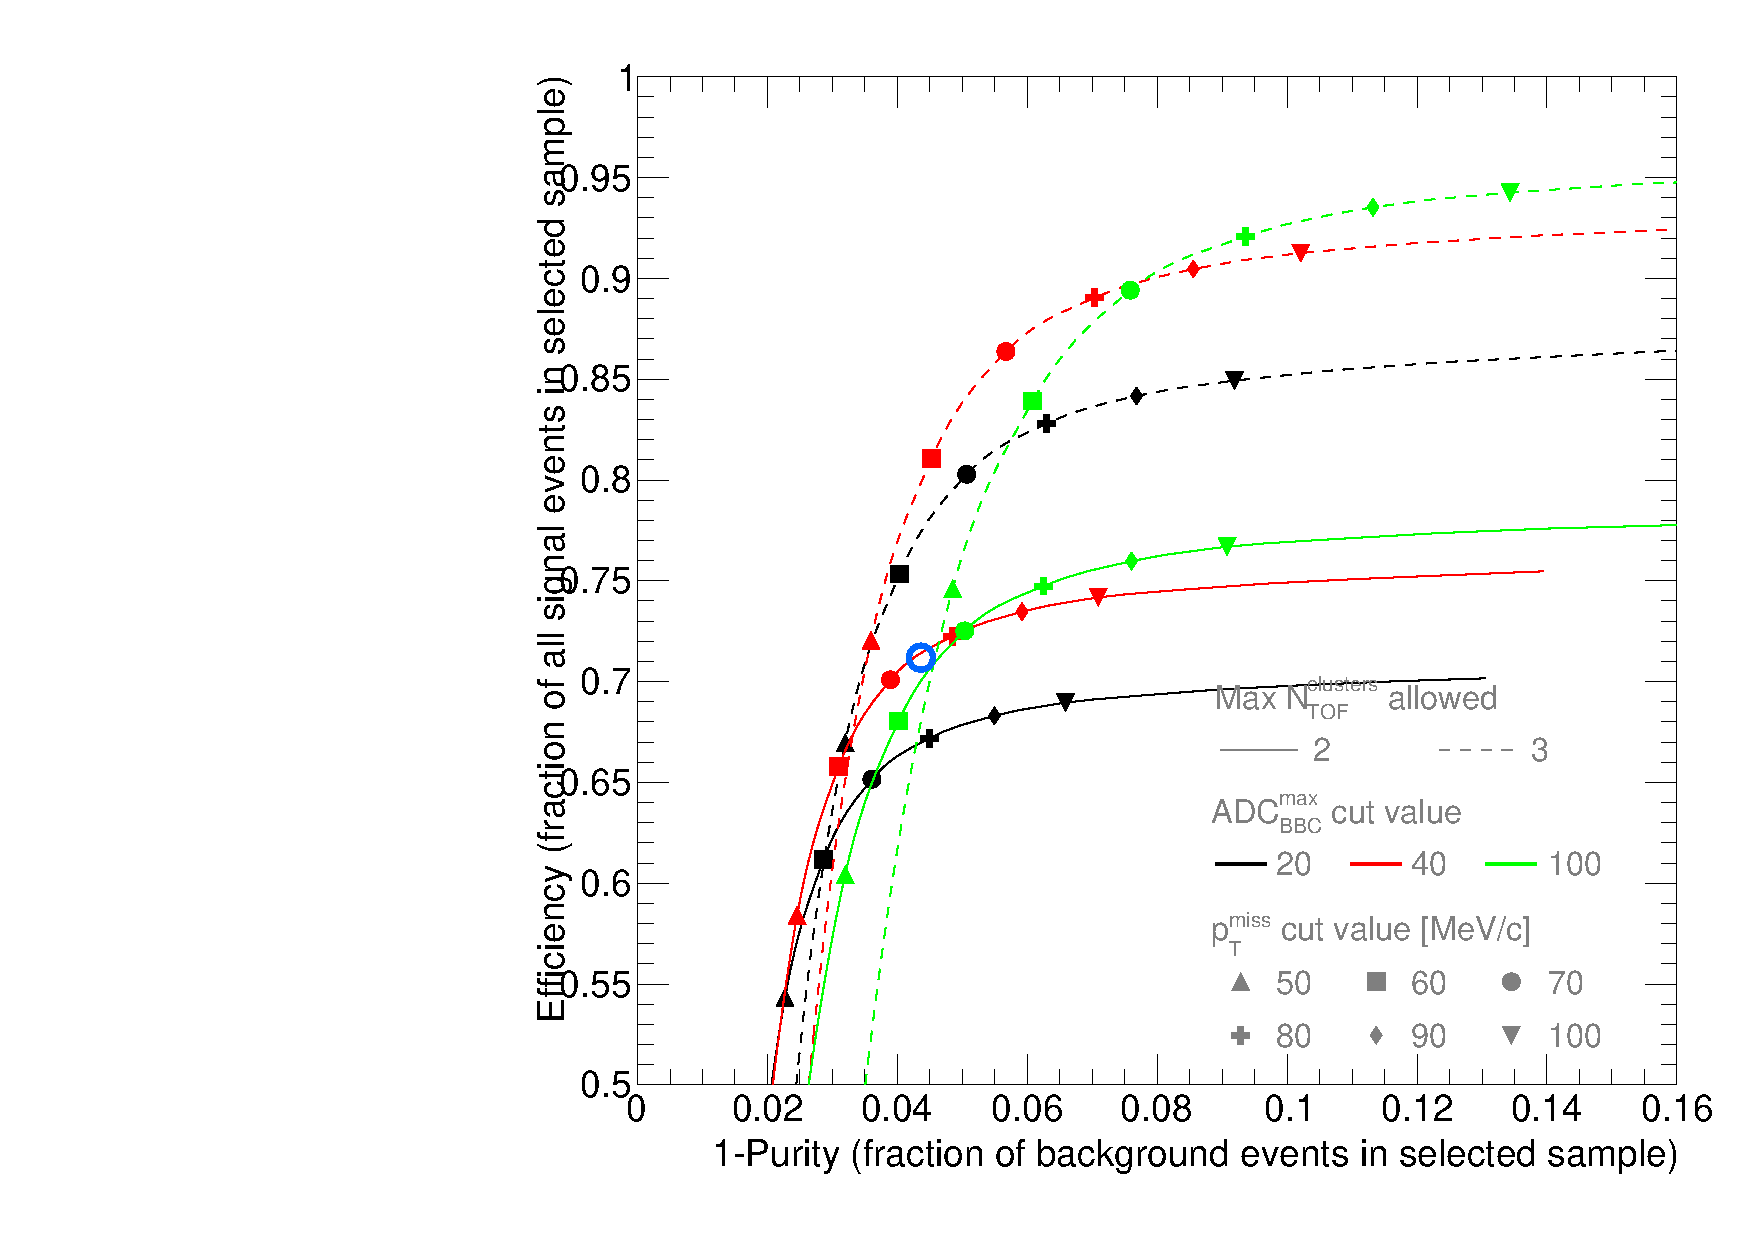
\includegraphics[width=\linewidth]{graphics/eventSelection/ROC_pTmiss.pdf}}
%   \end{subfigure}
% }%
% \quad\quad%
% \parbox{0.4725\textwidth}{
%   \centering
%   \begin{subfigure}[b]{\linewidth}\addtocounter{subfigure}{-2}
%                 \subcaptionbox{\label{fig:SignificanceVsBkgdFrac}}{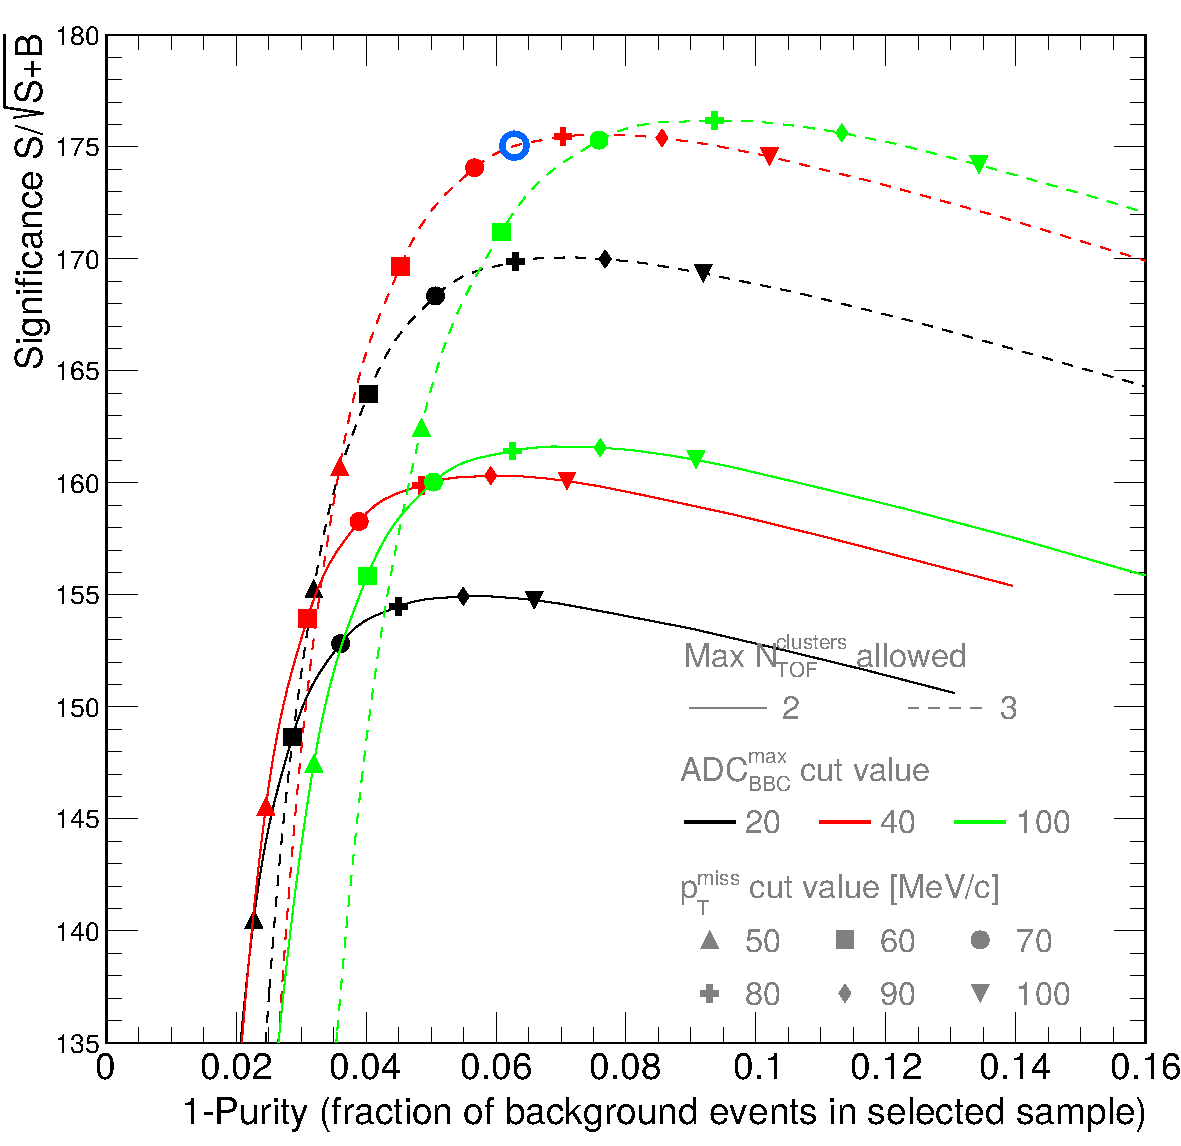
\includegraphics[width=\linewidth]{graphics/eventSelection/BkgdFractionVsEfficiency_pTmiss.pdf}}
%   \end{subfigure}\\
%   \begin{minipage}[t][1.042\linewidth][t]{\linewidth}\vspace{10pt}
%     \caption[Relation between $\pi^{+}\pi^{-}$ significance, efficiency and purity vs. thresholds in cuts~\ref{enum:CutBbcLarge}, \ref{enum:CutTofClusters} and \ref{enum:CutMissingPt}]{Relation between $\pi^{+}\pi^{-}$ signal significance and efficiency (\ref{fig:SignificanceVsEff}), significance and purity (\ref{fig:SignificanceVsBkgdFrac}), and efficiency and purity (\ref{fig:EffVsBkgdFrac}) as a function of cut thresholds in BBC-large veto (\ref{enum:CutBbcLarge}), TOF cluster limit (\ref{enum:CutTofClusters}) and exclusivity cut (\ref{enum:CutMissingPt}). Lines show forementioned relations with changing $p_{T}^\text{miss}$ cut whose some specific values are indicated with different markers. Color denotes ADC threshold in BBC-large veto (black, red or green). Style of line (solid or dashed) denotes $N^{\text{TOF}}_{\text{clstrs}}$ limit. Working point considered optimal is marked with opened blue circle.}\label{fig:workingPoint}
%   \end{minipage}
% }%
% 
% \end{figure}
% %--------------------------- 


% \section{Signal per integrated luminosity}
% 
% \section{Cut flow}\label{sec:cutFlow}
% 
% %---------------------------
% \begin{figure}[ht!]
% \centering%
% 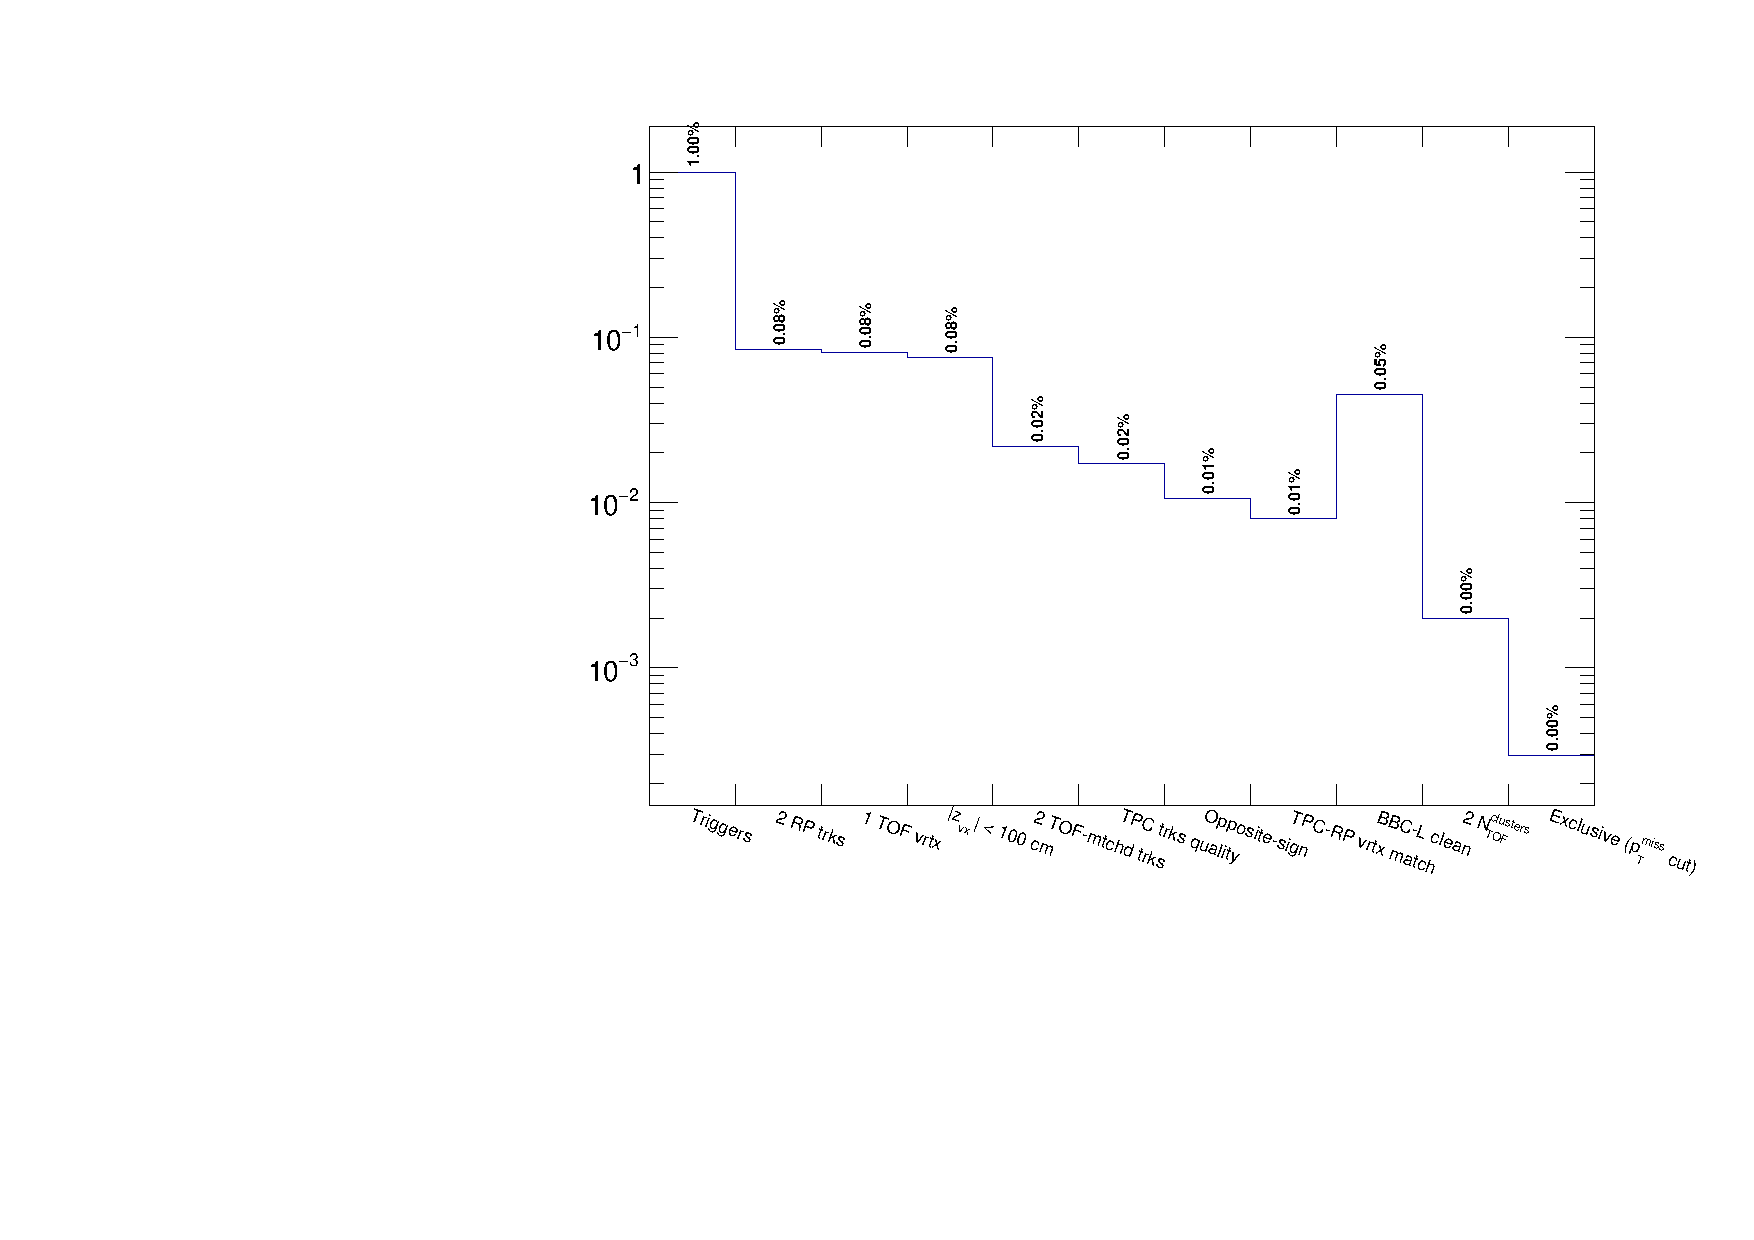
\includegraphics[width=0.85\linewidth,page=1]{graphics/eventSelection/CutFlow.pdf}%
% \caption{Cut flow.}\label{fig:CutFlow}%
% \end{figure}
% %---------------------------
